\documentclass{book}
\usepackage{blindtext}
\usepackage{hyperref}
\usepackage[margin=1.3in]{geometry}
\usepackage[scaled]{helvet}
\renewcommand\familydefault{\sfdefault}
\usepackage{verbatim, minted}
\usepackage[outputdir=build,cache=false]{minted}
\usepackage[T1]{fontenc}
\usepackage{graphicx}
\usepackage{ amssymb }
\usepackage{textcomp}
\usepackage{verbatim, graphicx, amsmath, mathtools, enumerate, hyperref, tcolorbox, newunicodechar, textgreek}
\usepackage{wasysym}
\usepackage{tipa}
\usepackage[demo]{graphicx} 
\usepackage{eso-pic} 
\usepackage{lipsum} 



\DeclareFontFamily{U}{min}{}
\DeclareFontShape{U}{min}{m}{n}{<-> udmj30}{}
\newcommand\yon{\!\text{\usefont{U}{min}{m}{n}\symbol{'210}}\!}

%BOLD FACE LETTERS
\DeclareUnicodeCharacter{1D538}{$\mathbbold{A}$}
\DeclareUnicodeCharacter{1D539}{$\mathbb{B}$}
\DeclareUnicodeCharacter{2144}{$\mathbbold{D}$}
\DeclareUnicodeCharacter{2102}{$\mathbb{C}$}
\DeclareUnicodeCharacter{2134}{$\mathbbold{E}$}
\DeclareUnicodeCharacter{2134}{$\mathbbold{F}$}
\DeclareUnicodeCharacter{2134}{$\mathbbold{G}$}
\DeclareUnicodeCharacter{2134}{$\mathbbold{H}$}
\DeclareUnicodeCharacter{2134}{$\mathbbold{I}$}
\DeclareUnicodeCharacter{2134}{$\mathbbold{J}$}
\DeclareUnicodeCharacter{2134}{$\mathbbold{K}$}
\DeclareUnicodeCharacter{2134}{$\mathbbold{L}$}
\DeclareUnicodeCharacter{2134}{$\mathbbold{M}$}
\DeclareUnicodeCharacter{2115}{$\mathbb{N}$}
\DeclareUnicodeCharacter{2134}{$\mathbbold{O}$}
\DeclareUnicodeCharacter{2134}{$\mathbbold{P}$}
\DeclareUnicodeCharacter{213}{$\mathbbold{Q}$}
\DeclareUnicodeCharacter{211D}{$\mathbb{R}$}
\DeclareUnicodeCharacter{2134}{$\mathbbold{S}$}
\DeclareUnicodeCharacter{2134}{$\mathbbold{T}$}
\DeclareUnicodeCharacter{2132}{$\mathbbold{U}$}
\DeclareUnicodeCharacter{2133}{$\mathbbold{V}$}
\DeclareUnicodeCharacter{2133}{$\mathbbold{W}$}
\DeclareUnicodeCharacter{2133}{$\mathbbold{X}$}
\DeclareUnicodeCharacter{2133}{$\mathbbold{Y}$}
\DeclareUnicodeCharacter{2124}{$\mathbbold{Z}$}
\usepackage{bbold}
\DeclareUnicodeCharacter{3087}{
\includegraphics[width=0.27cm,height=0.27cm]{yon.png}}%ょ 
\DeclareUnicodeCharacter{207B}{${}^{-}$}
\DeclareUnicodeCharacter{1D52}{${}^{\texttt{o}}$}
\DeclareUnicodeCharacter{1D56}{${}^{\texttt{p}}$}

\DeclareUnicodeCharacter{213F}{$\mathbb{\Pi}$}%

\DeclareUnicodeCharacter{1FAB2}{$$}

%CALIGRAPHY LETTERS
\DeclareUnicodeCharacter{1D4D0}{$\mathcal{A}$}%𝓐
\DeclareUnicodeCharacter{1D4D1}{$\mathcal{B}$}%𝓑
\DeclareUnicodeCharacter{1D4D2}{$\mathcal{C}$}%𝓒
\DeclareUnicodeCharacter{1D4D4}{$\mathcal{E}$}%𝓔
\DeclareUnicodeCharacter{1D4D5}{$\mathcal{F}$}%𝓕
\DeclareUnicodeCharacter{1D4D6}{$\mathcal{G}$}%𝓖
\DeclareUnicodeCharacter{1D4D7}{$\mathcal{H}$}%𝓗
\DeclareUnicodeCharacter{1D4D8}{$\mathcal{I}$}%𝓘
\DeclareUnicodeCharacter{1D4D9}{$\mathcal{J}$}%𝓙
\DeclareUnicodeCharacter{1D4DA}{$\mathcal{K}$}%𝓚
\DeclareUnicodeCharacter{1D4DB}{$\mathcal{L}$}%𝓛
\DeclareUnicodeCharacter{1D4DC}{$\mathcal{M}$}%𝓜
\DeclareUnicodeCharacter{1D4DD}{$\mathcal{N}$}%𝓝
\DeclareUnicodeCharacter{1D4DE}{$\mathcal{O}$}%𝓞
\DeclareUnicodeCharacter{1D4DF}{$\mathcal{P}$}%𝓟
\DeclareUnicodeCharacter{1D4E0}{$\mathcal{Q}$}%𝓠
\DeclareUnicodeCharacter{1D4E1}{$\mathcal{R}$}%𝓡
\DeclareUnicodeCharacter{1D4E2}{$\mathcal{S}$}%𝓢
\DeclareUnicodeCharacter{1D4E3}{$\mathcal{T}$}%𝓣
\DeclareUnicodeCharacter{1D4E4}{$\mathcal{U}$}%𝓤
\DeclareUnicodeCharacter{1D4E5}{$\mathcal{V}$}%𝓥
\DeclareUnicodeCharacter{1D4E6}{$\mathcal{W}$}%𝓦
\DeclareUnicodeCharacter{1D4E7}{$\mathcal{X}$}%𝓧
\DeclareUnicodeCharacter{1D4E8}{$\mathcal{Y}$}%𝓨
\DeclareUnicodeCharacter{1D4E9}{$\mathcal{Z}$}%𝓩


\DeclareUnicodeCharacter{2227}{$\wedge$}%∧
\DeclareUnicodeCharacter{2228}{$\vee$}%∨
%\DeclareUnicodeCharacter{2228}{}%¬



\DeclareUnicodeCharacter{21C4}{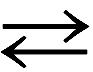
\includegraphics[width=0.27cm,height=0.27cm]{adj2.png}}%⇄

\DeclareUnicodeCharacter{1D7D9}{$\mathbb{1}$}%𝟙
\DeclareUnicodeCharacter{1D7ED}{$\bf{1}$}%𝟭


\DeclareUnicodeCharacter{2B62}{$\rightarrow$}%⭢

\DeclareUnicodeCharacter{2972}{$\stackrel{\sim}{→}$}%⥲

\DeclareUnicodeCharacter{FF08}{(}
\DeclareUnicodeCharacter{FF09}{)}

\DeclareUnicodeCharacter{221E}{$\infty$}


%CIRCLES
\DeclareUnicodeCharacter{2295}{$\oplus$}
\DeclareUnicodeCharacter{2297}{$\otimes$}
\DeclareUnicodeCharacter{235F}{$\oslash$}
\DeclareUnicodeCharacter{2D54}{$\ocircle$}%
\DeclareUnicodeCharacter{229A}{$\ocircle$}%⊚⊙⊜⊝
\DeclareUnicodeCharacter{2A36}{$\hat{\otimes}$}
\DeclareUnicodeCharacter{2A37}{$\hat{\otimes}$}
\DeclareUnicodeCharacter{2D41}{$\oslash$}%Unit

\DeclareUnicodeCharacter{0283}{$asdfasdfsdf$}%ʃ

\DeclareUnicodeCharacter{2245}{$\cong$}%≅

\DeclareUnicodeCharacter{29BE}{$\circledcirc$}
\DeclareUnicodeCharacter{29BF}{$\odot$}
\DeclareUnicodeCharacter{2218}{$\ensuremath{\circ}$}
\DeclareUnicodeCharacter{229B}{$\varoast$}


\DeclareUnicodeCharacter{2318}{$$}%⌘
\DeclareUnicodeCharacter{10779}{$\overline{\int}$}%⨛
\DeclareUnicodeCharacter{10779}{$\underline{\int}$}%⨜
\DeclareUnicodeCharacter{2A1B}{$\overline{\int}$}%⨛
\DeclareUnicodeCharacter{2A1C}{$\underline{\text{\textesh}}$}%⨜

\DeclareUnicodeCharacter{10527}{$\times$}%𐔧
\DeclareUnicodeCharacter{10527}{$\times$}%𐔧
\DeclareUnicodeCharacter{2A2F}{$\times$}%⨯
\DeclareUnicodeCharacter{8796}{$\stackrel{\triangle}{=}$}% ≜
\DeclareUnicodeCharacter{225C}{$\stackrel{\triangle}{=}$}%
\DeclareUnicodeCharacter{2259}{$\stackrel{\wedge}{=}$}%≙
\DeclareUnicodeCharacter{225A}{$\stackrel{\vee}{=}$}%≚
\DeclareUnicodeCharacter{225A}{$\stackrel{\circ}{=}$}%≗
\DeclareUnicodeCharacter{225B}{$\stackrel{*}{=}$}%≛
\DeclareUnicodeCharacter{2257}{$\stackrel{\circ}{=}$}%

\DeclareUnicodeCharacter{22A3}{$\vdash$}%𐔧

\DeclareUnicodeCharacter{2219}{$\bullet$}%

\DeclareUnicodeCharacter{2030}{${}_{=}$}%₌
\DeclareUnicodeCharacter{2030}{${}_{0}$}%₀
\DeclareUnicodeCharacter{2030}{${}_{1}$}%₁
\DeclareUnicodeCharacter{2030}{${}_{2}$}%₂
\DeclareUnicodeCharacter{2030}{${}_{3}$}%₃
\DeclareUnicodeCharacter{2030}{${}_{4}$}%₄
\DeclareUnicodeCharacter{2030}{${}_{5}$}%₅
\DeclareUnicodeCharacter{2030}{${}_{6}$}%₆
\DeclareUnicodeCharacter{2030}{${}_{7}$}%₇
\DeclareUnicodeCharacter{2030}{${}_{8}$}%₈
\DeclareUnicodeCharacter{2030}{${}_{9}$}%₉

\DeclareUnicodeCharacter{3088}{${
\includegraphics[width=0.27cm,height=0.27cm]{yon.png}}$}%₌


\DeclareUnicodeCharacter{279E}{$\raisebox{0.24ex}{
\includegraphics[width=0.34cm,height=0.15cm]{fun.png}}$}%
\DeclareUnicodeCharacter{21E8}{$\raisebox{0.24ex}{
\includegraphics[width=0.36cm,height=0.17cm]{nat.png}}$}%






%BRACES
\DeclareUnicodeCharacter{2983}{\lBrace}%⦃
\DeclareUnicodeCharacter{2984}{\rBrace}%⦄
\DeclareUnicodeCharacter{27E8}{$\langle$}%⟨
\DeclareUnicodeCharacter{27E9}{$\rangle$}%⟩
\DeclareUnicodeCharacter{300A}{}%《
\DeclareUnicodeCharacter{300B}{}%》 

\DeclareUnicodeCharacter{21C9}{
\includegraphics[width=0.27cm,height=0.27cm]{pair.png}}%

%Prd AND HOM OF category
\usepackage{bbm}

\DeclareUnicodeCharacter{1D569}{$\mathbb{x}$}%    𝕩
\DeclareUnicodeCharacter{27F9}{$\Rightarrow$}%    ⟹
\usepackage{ stmaryrd }
\DeclareUnicodeCharacter{27E6}{$\raisebox{0.15ex}{\llbracket}$}%        ⟦
\DeclareUnicodeCharacter{27E7}{$\raisebox{0.15ex}{\rrbracket}$}%        ⟧

\DeclareUnicodeCharacter{21D2}{$\Rightarrow$}%⇒

%COMMON CHARACTERS
\DeclareUnicodeCharacter{2A09}{$\times$}
\DeclareUnicodeCharacter{2218}{$\circ$}
\DeclareUnicodeCharacter{2261}{$\equiv$}
\DeclareUnicodeCharacter{21A6}{$\mapsto$}
\DeclareUnicodeCharacter{00D7}{$\times$}
\DeclareUnicodeCharacter{2202}{$\reflectbox{6}$}
\DeclareUnicodeCharacter{002A}{$asterisk$}
\DeclareUnicodeCharacter{21FE}{$\rightarrowtriangle$}
\DeclareUnicodeCharacter{27F6}{$\longrightarrow$}
\DeclareUnicodeCharacter{27F9}{$\Longrightarrow$}
\usepackage{dsfont}
\DeclareUnicodeCharacter{1D7D9}{$\mathds{1}$}
\DeclareUnicodeCharacter{2022}{$\bullet$}
\DeclareUnicodeCharacter{25B2}{$\triangledown$}
\DeclareUnicodeCharacter{25B3}{$\triangle$}
\DeclareUnicodeCharacter{25B4}{$\blacktriangledown$}%▴
\DeclareUnicodeCharacter{25BE}{$\blacktriangleup$}%▾
\DeclareUnicodeCharacter{25B5}{$\triangledown$}%▵
\DeclareUnicodeCharacter{2200}{$\forall$}
\DeclareUnicodeCharacter{2203}{$\exists$}



\DeclareUnicodeCharacter{2080}{${}_{\texttt{0}}$}
\DeclareUnicodeCharacter{2081}{${}_{\texttt{1}}$}
\DeclareUnicodeCharacter{2082}{${}_{\texttt{2}}$}
\DeclareUnicodeCharacter{2083}{${}_{\texttt{3}}$}
\DeclareUnicodeCharacter{2084}{${}_{\texttt{4}}$}
\DeclareUnicodeCharacter{2085}{${}_{\texttt{5}}$}
\DeclareUnicodeCharacter{2086}{${}_{\texttt{6}}$}
\DeclareUnicodeCharacter{2087}{${}_{\texttt{7}}$}
\DeclareUnicodeCharacter{2088}{${}_{\texttt{8}}$}
\DeclareUnicodeCharacter{2089}{${}_{\texttt{9}}$}

\DeclareUnicodeCharacter{21C6}{$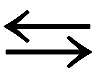
\includegraphics[width=0.29cm,height=0.29cm]{adj.png}$}



\makeatletter
\newcommand*{\shifttext}[2]{%
  \settowidth{\@tempdima}{#2}%
  \makebox[\@tempdima]{\hspace*{#1}#2}%
}
\makeatother

%INTEGRALS
\DeclareUnicodeCharacter{222C}{$\raisebox{0.3ex}{\scalebox{0.55}[0.86]{\raisebox{0.001ex}{\text{\textesh}}\shifttext{-3.6pt}{\text{\textesh}}}}$}%∬
\DeclareUnicodeCharacter{222E}{$\oint$}
\DeclareUnicodeCharacter{222D}{$\iiint$}
\DeclareUnicodeCharacter{222F}{$\oiint$}


\DeclareUnicodeCharacter{1F41C}{
\includegraphics[width=0.4cm,height=0.4cm]{ant}}%🐜
\DeclareUnicodeCharacter{1F347}{\includegraphics[width=0.4cm,height=0.4cm]{grapes.png}}%🍇
\DeclareUnicodeCharacter{1FAB2}{\includegraphics[width=0.6cm,height=0.4cm]{beetle.png}}%🪲
\DeclareUnicodeCharacter{1F40C}{\includegraphics[width=0.4cm,height=0.4cm]{snail.png}}%🐌
\DeclareUnicodeCharacter{1F34C}{\includegraphics[width=0.4cm,height=0.4cm]{banana.png}}%🍌
\DeclareUnicodeCharacter{1F353}{\includegraphics[width=0.4cm,height=0.4cm]{straw.png}}%🍓




\DeclareUnicodeCharacter{2116}{$\textnumero$}%№


\DeclareUnicodeCharacter{1D540}{$\mathbb{I}$}%𝕀

\DeclareUnicodeCharacter{0052}{$\mathbb{R}$}%ℝ
\DeclareUnicodeCharacter{0D54C}{$\mathbb{U}$}%𝕌
\DeclareUnicodeCharacter{1D555}{$\mathbb{d}$}%𝕕
\DeclareUnicodeCharacter{1D556}{$\mathbb{e}$}%𝕖
\DeclareUnicodeCharacter{1D55F}{$\mathbb{n}$}%𝕟
\DeclareUnicodeCharacter{1D564}{$\mathbb{s}$}%𝕤

\DeclareUnicodeCharacter{1D4D1}{$\mathcal{B}$}%𝓑 
\DeclareUnicodeCharacter{1D4D2}{$\mathcal{C}$}%𝓒 
\DeclareUnicodeCharacter{1D4D3}{$\mathcal{D}$}%𝓓 
\DeclareUnicodeCharacter{1D4D4}{$\mathcal{E}$}%𝓔 
\DeclareUnicodeCharacter{1D4D5}{$\mathcal{F}$}%𝓕 
\DeclareUnicodeCharacter{1D4D6}{$\mathcal{G}$}%𝓖
\DeclareUnicodeCharacter{1D4D6}{$\mathcal{H}$}%𝓗

\DeclareUnicodeCharacter{0302}{\raisebox{0.45ex}{\shifttext{-15.2pt}{$\textasciicircum$}}}%𝕤


%𝕀𝕟𝕕,ℝ𝕖𝕤,Locus

\DeclareUnicodeCharacter{1D543}{$\mathbb{L}$}%𝕃
\DeclareUnicodeCharacter{1D560}{$\mathbb{o}$}%𝕠
\DeclareUnicodeCharacter{1D554}{$\mathbb{c}$}%𝕔
\DeclareUnicodeCharacter{1D566}{$\mathbb{u}$}%𝕦
\DeclareUnicodeCharacter{1D564}{$\mathbb{s}$}%𝕤
\DeclareUnicodeCharacter{222B}{$\text{\textesh}$}

\DeclareUnicodeCharacter{1BC94}{$\raisebox{0.05ex}{{}_{\resizebox{0.07in}{!}{\cdot}}}$}%𛲔 
\DeclareUnicodeCharacter{0971}{$\raisebox{-.23ex}{{}^{\resizebox{0.07in}{!}{\cdot}}}$}%ॱ
\DeclareUnicodeCharacter{02024}{${}^{\cdot}$}% ․ 

\DeclareUnicodeCharacter{0207A}{${}^{+}$}%⁺
\DeclareUnicodeCharacter{0208A}{${}_{+}$}%₊






\definecolor{Red}{cmyk}{0.1, 0.70, 0.65, 0.00, 1.00}
\definecolor{Blue}{cmyk}{0.70, 0.08, 0.08, 0.04, 1.00}
\definecolor{Yellow}{cmyk}{0.0, 0.00, 0.7, 0.00, 0.5}
\definecolor{Green}{cmyk}{0.6, 0.0, 0.6, 0.00, 1.00}
\definecolor{Purple}{cmyk}{0.8, 0.3, 0.3, 0.00, 1.00}
\definecolor{Orange}{cmyk}{0.0, 0.3, 0.7, 0.00, 1.00}

%LEAN counter
\newcounter{definitioncounter}
\setcounter{definitioncounter}{1}

%Theorem counter
\newcounter{theoremcounter}
\setcounter{theoremcounter}{1}

%Print counter
\newcounter{printcounter}
\setcounter{printcounter}{1}

%Example counter
\newcounter{examplecounter}
\setcounter{examplecounter}{1}

%Example counter
\newcounter{ccounter}
\setcounter{ccounter}{1}

%Print counter
\newcounter{pcounter}
\setcounter{pcounter}{1}

%Print counter
\newcounter{lcounter}
\setcounter{lcounter}{1}

\usepackage[T1]{fontenc}

\newcounter{sectioncount}
\newcounter{subsectioncount}
\setcounter{sectioncount}{1}
\renewcommand{\section}[1]{\newpage
\ \\
\ \\
 \begin{center} \scalebox{1.5}{\texttt{\thesectioncount . #1}} \setcounter{sectioncount}{\thesectioncount+1} \setcounter{subsectioncount}{1} \end{center}
 \begin{center}

\ \\
\ \\

\thispagestyle{empty}
\end{center}
}

\renewcommand{\subsection}[1]{\texttt{\thesubsectioncount . #1} \setcounter{subsectioncount}{\thesubsectioncount+1}}
\begin{document}

\AddToShipoutPicture*
    {\put(535,720){

    \href{http://www.linearlibrary.net}{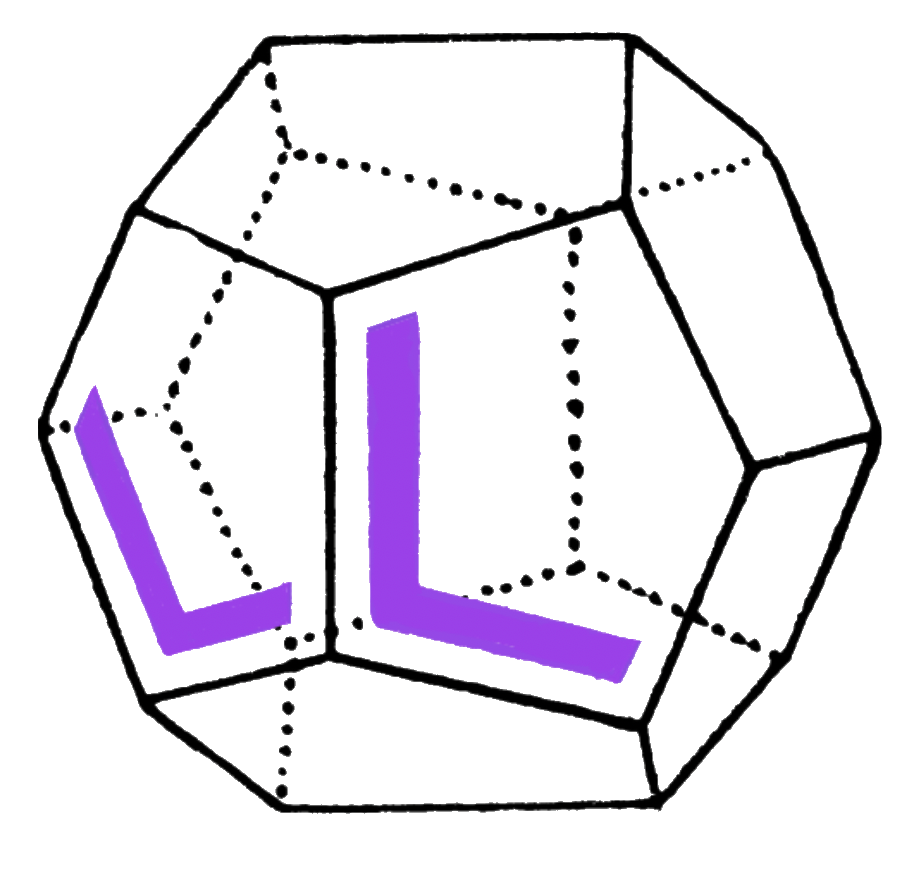
\includegraphics[width=2cm,height=2cm]{ll.png}}

    }}

\AddToShipoutPicture*
  {\put(475,737){

    \href{http://www.linearlibrary.net/CategoryTheory.pdf}{\texttt{.pdf file}}\\

  }}

\AddToShipoutPicture*
  {\put(475,752){
    \href{http://www.linearlibrary.net/CategoryTheory.tex}{\texttt{.tex file}}\\

  }}

\AddToShipoutPicture*
  {\put(475,767){
    \href{http://www.linearlibrary.net/CategoryTheory.py}{\texttt{.py file}}

  }}

\AddToShipoutPicture*
  {\put(475,722){
    \href{http://www.linearlibrary.net/CategoryTheory.lean}{\texttt{.lean file}}

  }}



\pagecolor{Purple}

\begin{center}

\ \\
\ \\
\ \\
\ \\
\ \\
\ \\
\ \\
\ \\
\ \\

%LEAN: 
\begin{center}
\begin{tcolorbox}[width=3.7in,colback={Blue},colbacktitle=Blue,coltitle=black]
\scalebox{4.52}{\texttt{CATEGORIES}}
\end{tcolorbox}
\end{center}

\begin{center}
\texttt{String diagrams in Lean 4}\\
\ \\
\ \\
\ \\
\includegraphics[width=4cm,height=5.5cm]{cover.png}
\ \\
\ \\
\texttt{Elliot Young}
\ \\
\end{center}


\ \\
\ \\
\end{center}
\thispagestyle{empty}
\newpage
\pagecolor{white}
\color{black}
\ \\
\ \\
\thispagestyle{empty}
\begin{center}
\iffalse
Copyright\ \textcopyright \ 2023 Elliot Dean Young.\ All rights reserved.\\
\fi
\end{center}


\newpage


\section{Introduction}

The main goals of this text are to prove:

\begin{center}
\begin{tabular}{|l|}
\hline
\multicolumn{2}{|c|}{\texttt{Main Goals}} \\
\hline
\hline
Proving Fox's theorem  \\
\hline
Proving the Yoneda lemma \\
\hline
Proving the adjoint functor theorem \\
\hline
Proving the Isbell duality isomorphism\\
\hline
\end{tabular}
\end{center}

Special effort has been made to make it approachable and self-contained. All of the theorems and proofs will be written in Lean 4. It also contains graphics called string diagrams. See the \href{https://github.com/leanprover/lean4}{Lean 4 Github} for installation instructions detailing how to get started with Lean 4, or \href{https://lean.math.hhu.de/#code=--\%20some\%20essentials\%0A\%0Adef\%20extensionality\%20(f\%20g\%20\%3A\%20X\%20\%E2\%86\%92\%20Y)\%20(p\%20\%3A\%20(x\%3AX)\%20\%E2\%86\%92\%20f\%20x\%20\%3D\%20g\%20x)\%20\%3A\%20f\%20\%3D\%20g\%20\%3A\%3D\%20funext\%20p\%0Adef\%20equal_arguments\%20\%7BX\%20\%3A\%20Type\%7D\%20\%7BY\%20\%3A\%20Type\%7D\%20\%7Ba\%20\%3A\%20X\%7D\%20\%7Bb\%20\%3A\%20X\%7D\%20(f\%20\%3A\%20X\%20\%E2\%86\%92\%20Y)\%20(p\%20\%3A\%20a\%20\%3D\%20b)\%20\%3A\%20f\%20a\%20\%3D\%20f\%20b\%20\%3A\%3D\%20congrArg\%20f\%20p\%0Adef\%20equal_functions\%20\%7BX\%20\%3A\%20Type\%7D\%20\%7BY\%20\%3A\%20Type\%7D\%20\%7Bf\%E2\%82\%81\%20\%3A\%20X\%20\%E2\%86\%92\%20Y\%7D\%20\%7Bf\%E2\%82\%82\%20\%3A\%20X\%20\%E2\%86\%92\%20Y\%7D\%20(p\%20\%3A\%20f\%E2\%82\%81\%20\%3D\%20f\%E2\%82\%82)\%20(x\%20\%3A\%20X)\%20\%3A\%20f\%E2\%82\%81\%20x\%20\%3D\%20f\%E2\%82\%82\%20x\%20\%3A\%3D\%20congrFun\%20p\%20x\%0A\%0Adef\%20reflexivity\%20\%7BX\%20\%3A\%20Type\%7D\%20\%7Bx\%20\%3A\%20X\%7D\%20(p\%20\%3A\%20x\%20\%3D\%20x)\%20\%3A\%3D\%20Eq.refl\%20p\%0Adef\%20symmetry\%20\%7BX\%20\%3A\%20Type\%7D\%20\%7Bx\%20\%3A\%20X\%7D\%20\%7By\%20\%3A\%20X\%7D\%20\%20(p\%20\%3A\%20x\%20\%3D\%20y)\%20\%3A\%3D\%20Eq.symm\%20p\%0Adef\%20transitivity\%20\%7BX\%20\%3A\%20Type\%7D\%20\%7Bx\%20\%3A\%20X\%7D\%20\%7By\%20\%3A\%20X\%7D\%20\%7Bz\%20\%3A\%20X\%7D\%20(p\%20\%3A\%20x\%20\%3D\%20y)\%20(q\%20\%3A\%20y\%20\%3D\%20z)\%20\%3A\%3D\%20Eq.trans\%20p\%20q\%0Anotation\%20p\%20\%22\%7C\%22\%20q\%20\%3D\%3E\%20transitivity\%20p\%20q\%0A\%0A\%0A--\%20A\%20category\%20C\%20consists\%20of\%3A\%0Astructure\%20category\%20where\%0A\%20\%20Obj\%20\%3A\%20Type\%20u\%0A\%20\%20Hom\%20\%3A\%20Obj\%20\%E2\%86\%92\%20Obj\%20\%E2\%86\%92\%20Type\%20v\%0A\%20\%20Idn\%20\%3A\%20(X\%3AObj)\%20\%E2\%86\%92\%20Hom\%20X\%20X\%0A\%20\%20Cmp\%20\%3A\%20(X\%3AObj)\%20\%E2\%86\%92\%20(Y\%3AObj)\%20\%E2\%86\%92\%20(Z\%3AObj)\%20\%E2\%86\%92\%20(_\%3AHom\%20X\%20Y)\%20\%E2\%86\%92\%20(_\%3AHom\%20Y\%20Z)\%20\%E2\%86\%92\%20Hom\%20X\%20Z\%0A\%20\%20Id\%E2\%82\%81\%20\%3A\%20(X\%3AObj)\%20\%E2\%86\%92\%20(Y\%3AObj)\%20\%E2\%86\%92\%20(f\%3AHom\%20X\%20Y)\%20\%E2\%86\%92\%20\%0A\%20\%20\%20\%20Cmp\%20X\%20Y\%20Y\%20f\%20(Idn\%20Y)\%20\%3D\%20f\%0A\%20\%20Id\%E2\%82\%82\%20\%3A\%20(X\%3AObj)\%20\%E2\%86\%92\%20(Y\%3AObj)\%20\%E2\%86\%92\%20(f\%3AHom\%20X\%20Y)\%20\%E2\%86\%92\%20\%0A\%20\%20\%20\%20Cmp\%20X\%20X\%20Y\%20(Idn\%20X)\%20f\%20\%3D\%20f\%0A\%20\%20Ass\%20\%3A\%20(W\%3AObj)\%20\%E2\%86\%92\%20(X\%3AObj)\%20\%E2\%86\%92\%20(Y\%3AObj)\%20\%E2\%86\%92\%20(Z\%3AObj)\%20\%E2\%86\%92\%20(f\%3AHom\%20W\%20X)\%20\%E2\%86\%92\%20(g\%3AHom\%20X\%20Y)\%20\%E2\%86\%92\%20(h\%3AHom\%20Y\%20Z)\%20\%E2\%86\%92\%0A\%20\%20\%20\%20(Cmp\%20W\%20X\%20Z)\%20f\%20(Cmp\%20X\%20Y\%20Z\%20g\%20h)\%20\%3D\%20Cmp\%20W\%20Y\%20Z\%20(Cmp\%20W\%20X\%20Y\%20f\%20g)\%20h\%0A\%0A\%0A--\%20Notation\%20for\%20the\%20identity\%20map\%20which\%20infers\%20the\%20category\%3A\%0Adef\%20identity_map\%20\%7BC\%20\%3A\%20category\%7D\%20(X\%20\%3A\%20C.Obj)\%20\%3A\%3D\%20C.Idn\%20X\%0Anotation\%20\%22\%F0\%9D\%9F\%99\%22\%20\%3D\%3E\%20identity_map\%0A\%0A--\%20Notation\%20for\%20the\%20domain\%20of\%20a\%20morphism\%3A\%0Adef\%20Dom\%20\%7BC\%20\%3A\%20category\%7D\%20\%7BX\%20\%3A\%20C.Obj\%7D\%20\%7BY\%20\%3A\%20C.Obj\%7D\%20(_\%20\%3A\%20C.Hom\%20X\%20Y)\%20\%3A\%3D\%20X\%0A\%0A--\%20Notation\%20for\%20the\%20codomain\%20of\%20a\%20morphism\%3A\%0Adef\%20Cod\%20\%7BC\%20\%3A\%20category\%7D\%20\%7BX\%20\%3A\%20C.Obj\%7D\%20\%7BY\%20\%3A\%20C.Obj\%7D\%20(_\%20\%3A\%20C.Hom\%20X\%20Y)\%20\%3A\%3D\%20X\%0A\%0A\%0A--\%20Notation\%20for\%20composition\%20which\%20infers\%20the\%20category\%20and\%20objects\%3A\%0Adef\%20composition\%20\%7BC\%20\%3A\%20category\%7D\%20\%7BX\%20\%3A\%20C.Obj\%7D\%20\%7BY\%20\%3A\%20C.Obj\%7D\%20\%7BZ\%20\%3A\%20C.Obj\%7D\%20(f\%20\%3A\%20C.Hom\%20X\%20Y)\%20(g\%20\%3A\%20C.Hom\%20Y\%20Z)\%20\%3A\%20C.Hom\%20X\%20Z\%20\%3A\%3D\%20C.Cmp\%20X\%20Y\%20Z\%20f\%20g\%0A}{try this example.}\\

Mathematics is one of the oldest subjects, and as it concerns computer proof assistants, this entails a kind of change and development which is slow. Being in a subject where we are so commonly reminded of the brilliant minds who know things we do not, we have learned to defer to those who seem to have developed better judgement. At times this breeds specialization, at others, deference to talent, wisdom, or maturity.\\

This approach comes with many flaws, and we may have had higher hopes for decentralization in the Queen of the Sciences. Possibly computers will allow for a flexible higher mathematics which is more provisional where it should be, perminant in areas where an approach is insusceptible of improvement.\\

This much is not to mention the seemingly inevitable advent of an artificial intelligence which can outperform mathematicians at mathematics. Since this advent lies indefinitely far into the future, we might instead consider nearer benchmarks, each more tractible in one or another way. We may look forward to high quality search engines for mathematics, for instance.\\

Conglomerate interest itself is a meaningful factor in the development of computer proof assistants, and we should be wary of those who align themselves against its long term benefits. In any case, being part of these critical moments in the history of one of the oldest subjects makes mathematics all the more exciting.\\


\newpage
%Last day I added or deleted a Lean environment: April 18th
\section{Contents}

{\small
\begin{center}
\begin{tabular}{|l | l |} 
\hline
$\texttt{Section}$ & $\texttt{Description}$ \\
\hline \hline
\multicolumn{2}{|c|}{\texttt{Chapter I: the cartesian closed category of categories}} \\
\hline \hline
\texttt{category} &\ the category structure\\
\hline
\texttt{Cat} &\ the category of categories\\
\hline
\texttt{ᵒᵖ} &\ the opposite category\\
\hline \hline
\multicolumn{2}{|c|}{\texttt{Chapter II: the cartesian closed category of categories}} \\
\hline \hline
\texttt{C × D} &\ the product category \texttt{C × D} for \texttt{C, D : category} \\
\hline
\texttt{[C, D]} &\ the functor category \texttt{[C, D]} for \texttt{C, D : category} \\
\hline 
\texttt{C × - : Cat ➞ Cat} &\ the functor \texttt{C × - : Cat ➞ Cat} for \texttt{C : category}\\
\hline
\texttt{[C , -] : Cat ➞ Cat} &\ the functor \texttt{[C, -] : Cat ➞ Cat} for \texttt{C : category}  \\ 
\hline
\texttt{- × C ⊣ [C, -], η, ε} &\ the adjunction \texttt{- × C ⊣ [C, -], η, ε} for \texttt{C : category} \\
\hline
\texttt{- × C, τ, Δ} &\ the comonad \texttt{- × C, τ, Δ} for \texttt{C : category}  \\
\hline
\texttt{[C, -], ι, μ} &\ the monad \texttt{[C, -], ι, μ} for \texttt{C : category}  \\
\hline
\texttt{(- × C) • (- × D) ≅ (- × D) • (- × C)} &\ commutativity of \texttt{- × C} and \texttt{- × D} for \texttt{C, D : ategory} \\ 
\hline 
\texttt{[C,-] • [D,-] ≅ [D,-] • [C,-]} &\ commutativity of \texttt{[C, -]} and \texttt{[D, -]} for \texttt{C, D : category} \\
\hline
\texttt{⊛} &\ the category \texttt{⊛} \\
\hline
\texttt{Prd ⊛ ≅ 𝟭 Cat} &\ the identity law for the product \\
\hline
\texttt{Hom ⊛ ≅ 𝟭 Cat} &\ the identity law for the functor category \\
\hline
Fox's Theorem &\ a characterization of cartesian closed categories \\
\hline \hline
\multicolumn{2}{|c|}{\texttt{Chapter IV: the (strict) twocategory of categories}} \\
\hline
\hline
\texttt{twocategory} &\ the (strict) twocategory structure \\
\hline
\texttt{Two} &\ the twocategory of categories \\
\hline
• &\ notation for horizontal composition \\
\hline
\hline
\multicolumn{2}{|c|}{\texttt{Chapter V: sets and the Yoneda lemma}} \\
\hline
\hline 
\texttt{Set} &\ the category of sets\\
\hline
ょ &\ the Yoneda embedding and the Yoneda lemma \\
\hline 
\hline
\multicolumn{2}{|c|}{\texttt{Chapter VI: adjunctions, monads, and comonads}} \\
\hline
\hline
$\texttt{adjunction}$ &\ adjunctions \\
\hline
$\texttt{monad}$ &\ monads \\
\hline
$\texttt{comonad}$ &\ comonads \\
\hline
$\texttt{monadicity}$ &\ monadicity of an adjunction \\
\hline
$\texttt{comonadicity}$ &\ comonadicity of an adjunction \\
\hline
\end{tabular}
\end{center}}

{\small
\begin{center}
\begin{tabular}{|l | l |} 
\hline
\multicolumn{2}{|c|}{\texttt{Chapter VII: limits and colimits}} \\
\hline
\hline
$\texttt{lim I C:[I,C]⇆C}$  &\ the definition of limit \\
\hline
$\texttt{colim I C:[I,C]⇄C}$  &\ the definition of colimit \\
\hline
$\texttt{lim (Dis X) : [(Dis X),Set]⇄Set}$  &\ the limit with a set as a diagram in $\texttt{Set}$ \\
\hline  
$\texttt{colim (Dis X) : [(Dis X),Cat]⇄Cat}$  &\ the limit with a set a diagram in $\texttt{Cat}$ \\
/ \hline  
\texttt{⇉}  &\ The category with two parallel morphisms $\texttt{⇉}$\\
\hline
$\texttt{lim ⇉ Set}$ &\ limits over the category $\texttt{⇉}$ \\
\hline
$\texttt{colim ⇉ Set}$ &\ colimits over the category $\texttt{⇉}$ \\
\hline 
$\texttt{lim ⇉ Cat}$ &\ limits over the category $\texttt{⇉}$ in $\texttt{Cat}$ \\
\hline
$\texttt{colim ⇉ Cat}$ &\ limits over the category $\texttt{⇉}$ in $\texttt{Cat}$ \\
\hline
$\texttt{lim C U}$ &\ limits are equilizers of particular products \\
\hline
$\texttt{colim C U}$ &\ colimits are coequilizers of particular coproducts \\
\hline
\hline
\multicolumn{2}{|c|}{\texttt{Chapter VIII: the adjoint functor theorem}} \\
\hline
\hline
$\texttt{el F}$ & the category of elements of a functor $\text{F : C ➞ D}$\\
\hline
$\texttt{colim G • (el F) = G × F}$ & - everything is a colimit of representables\\
\hline
$\texttt{lim G • (el F) = Hom G F}$ & - \\
\hline
\end{tabular}
\end{center}}


\iffalse
 {
\small
\begin{center}
\begin{tabular}{|l | l |}
\multicolumn{2}{|c|}{\texttt{Chapter VII: pullbacks and pushouts}} \\
\hline
\hline
$\texttt{bijunction C Bij}$ &\
- certainly a bijunction representation is enough.
\hline
\hline
\multicolumn{2}{|c|}{\texttt{Chapter VIII: 0 ➞ ℕ ➞ Eℕ ➞ Bℕ ➞ 0}} \\
\hline
\hline
\texttt{ℕ}  &\ The discrete category with $\texttt{ℕ}$ as objects \\
\hline
\texttt{Eℕ} &\ The total space of $\texttt{ℕ}$  \\
\hline
\texttt{Bℕ} &\ The classifying space of $\texttt{ℕ}$ \\
\hline
\texttt{0 ➞ ℕ ➞ Eℕ ➞ Bℕ ➞ 0} &\ \texttt{Eℕ} is a covering space of \texttt{Bℕ} with fibers \texttt{ℕ}\\
\hline
\texttt{lim ℕ Cat : [ℕ, Cat] ⇆ Cat} &\ \texttt{Eℕ} is a covering space of \texttt{Bℕ} with fibers \texttt{ℕ}\\
\hline
\texttt{lim Eℕ Cat : [Eℕ, Cat] ⇆ Cat} &\ limit with \texttt{Eℕ} as a diagram\\
\hline
\texttt{lim Bℕ Cat : [Bℕ, Cat] ⇆ Cat} &\ limit with \texttt{Bℕ} as a diagram\\
\hline
\texttt{colim ℕ Cat : [ℕ, Cat] ⇄ Cat} &\ \texttt{Eℕ} is a covering space of \texttt{Bℕ} with fibers \texttt{ℕ}\\
\hline
\texttt{colim Eℕ Cat : [Eℕ, Cat] ⇄ Cat} &\ \texttt{Eℕ} is a covering space of \texttt{Bℕ} with fibers \texttt{ℕ}\\
\hline
\texttt{colim Bℕ Cat : [Bℕ, Cat] ⇄ Cat} &\ \texttt{Eℕ} is a covering space of \texttt{Bℕ} with fibers \texttt{ℕ}\\
\hline
\end{tabular}
\end{center}
}
\fi

\newpage
\newpage

\section{Lean 4}

Before we get started defining what a category is, we will cover the basic features of types in Lean 4. The main way we tell Lean 4 what something means is with $\texttt{def}$, which defines a term in dependent type theory. Much in the same way as other computer languages, we then supply the type of the term:

%LEAN: 
\begin{center}
\begin{tcolorbox}[width=5in,colback={white},title={\begin{center}\texttt{Lean \thelcounter} \addtocounter{lcounter}{1}  \end{center}},colbacktitle=Blue,coltitle=black]
\begin{minted}[breaklines, escapeinside=||]{lean}

def n : Int := 1

\end{minted}%
\end{tcolorbox}
\end{center}

here we have introduced an integer $\texttt{n}$ using the type $\texttt{Int}$ that comes with Lean 4. The main feature of a type besides a fascility with dependent product and hom is equality. This satisfies the three properties of an equivalence relation:

%LEAN: 
\begin{center}
\begin{tcolorbox}[width=5in,colback={white},title={\begin{center}\texttt{Lean \thelcounter} \addtocounter{lcounter}{1}  \end{center}},colbacktitle=Blue,coltitle=black]
\begin{minted}[breaklines, escapeinside=||]{lean}

def reflexivity {X : Type} {x : X} (p : x = x) := Eq.refl p
def symmetry {X : Type} {x : X} {y : X}  (p : x = y) := Eq.symm p
def transitivity {X : Type} {x : X} {y : X} {z : X} (p : x = y) (q : y = z) := Eq.trans p q
notation p "|" q => transitivity p q

\end{minted}%
\end{tcolorbox}
\end{center}

We must also require that functiosn satisfy extensionality:

%LEAN: some essential features of equality
\begin{center}
\begin{tcolorbox}[width=5in,colback={white},title={\begin{center}\texttt{Lean \thelcounter} \addtocounter{lcounter}{1}  \end{center}},colbacktitle=Blue,coltitle=black]
\begin{minted}[breaklines, escapeinside=||]{lean}

def extensionality (f g : X → Y) (p : (x:X) → f x = g x) : f = g := funext p

\end{minted}%
\end{tcolorbox}
\end{center}

Extensionality says that functions which are equal on all values are themselves equal, and it is featured in what is perhaps the most famous mathematical foundations, ZFC.

There are two other features of equality with respect to functions which we should be aware of:

%LEAN: 
\begin{center}
\begin{tcolorbox}[width=5in,colback={white},title={\begin{center}\texttt{Lean \thelcounter} \addtocounter{lcounter}{1}  \end{center}},colbacktitle=Blue,coltitle=black]
\begin{minted}[breaklines, escapeinside=||]{lean}

def equal_arguments {X : Type} {Y : Type} {a : X} {b : X} (f : X → Y) (p : a = b) : f a = f b := congrArg f p

def equal_functions {X : Type} {Y : Type} {f₁ : X → Y} {f₂ : X → Y} (p : f₁ = f₂) (x : X) : f₁ x = f₂ x := congrFun p x

\end{minted}%
\end{tcolorbox}
\end{center}
These are the only features of equality which we will need.\\

The tutorial \href{https://leanprover.github.io/theorem_proving_in_lean4/}{here} provides a good introduction to using the dependent type theory in Lean.

\newpage
\ \\
{
\Huge 
\begin{center}
\texttt{Chapter I : categories}
\end{center}
\thispagestyle{empty}
}

\ \\
\ \\
\ \\
\ \\

{
\small
\begin{center}
\begin{tabular}{|l | l |} 
 \hline
 $\texttt{Section}$ & $\texttt{Description}$ \\
 \hline \hline
 \texttt{category} &\ the category structure \\ 
 \hline
 \texttt{Cat} &\ the category of categories \\
 \hline
 \texttt{C × D} &\ the product category \texttt{C × D} for \texttt{C, D : category} \\
 \hline
 \texttt{[C, D]} &\ the functor category \texttt{[C, D]} for \texttt{C, D : category} \\
 \hline 
 \texttt{C × - : Cat ➞ Cat} &\ the functor \texttt{C × - : Cat ➞ Cat} for \texttt{C : category}\\
 \hline
 \texttt{[C , -] : Cat ➞ Cat} &\ the functor \texttt{[C, -] : Cat ➞ Cat} for \texttt{C : category}  \\ 
 \hline
 \texttt{- × C ⊣ [C, -], η, ε} &\ the adjunction \texttt{- × C ⊣ [C, -], η, ε} for \texttt{C : category} \\
 \hline
 \texttt{- × C, τ, Δ} &\ the comonad \texttt{- × C, τ, Δ} for \texttt{C : category}  \\
 \hline
 \texttt{[C, -], ι, μ} &\ the monad \texttt{[C, -], ι, μ} for \texttt{C : category}  \\
 \hline
 \texttt{(- × C) • (- × D) ≅ (- × D) • (- × C)} &\ commutativity of \texttt{- × C} and \texttt{- × D} for \texttt{C, D : category} \\
 \hline 
 \texttt{[C,-] • [D,-] ≅ [D,-] • [C,-]} &\ commutativity of \texttt{[C, -]} and \texttt{[D, -]} for \texttt{C, D : category} \\
 \hline
 \texttt{⊛, ⊛ × - ≅ 𝟭 Cat, [⊛, -] ≅ 𝟭 Cat} &\ the unit category \texttt{⊛} and identity laws \\
 \hline
 Fox's Theorem &\ a characterization of cartesian closed categories \\
 \hline
\end{tabular}
\end{center}
}

\section{\texttt{category}}

Our first goal is to define categories along with some notation for them. Categories were invented my Samuel Eilenberg and Saunders Mac Lane in the 20th century in the course of the work in algebraic topology. A category is a seven tuple consisting of:
\begin{enumerate}
\item A class $\texttt{Obj}$ of objects
\item For each pair of objects $\texttt{X,Y:Obj}$, a class $\texttt{Hom}$ whose elements are called morphisms. 
\item For each object $\texttt{X}$, a morphism $\texttt{Idn X}$, also written $\texttt{1}_{\texttt{X}}$.
\item For each triple of objects $\texttt{X, Y, Z : Obj}$, a function $\texttt{(Hom X Y) × (Hom Y Z) → (Hom X Z)}$.
\end{enumerate}
such that
\begin{enumerate}
\item $\texttt{∀(X:Obj),∀(Y:Obj),∀(f:Hom X Y),}$
\[\texttt{f∘(Idn X)=f}\]
\item $\texttt{∀(X:Obj),∀(Y:Obj),∀(f:Hom X Y),(Idn X)∘f=f}$
\[\texttt{(Idn X)∘f=f}\]
\item $\texttt{∀(W:Obj),∀(X:Obj),∀(Y:Obj),∀(Z : Obj),∀(f:Hom W X),∀(g:Hom X Y),∀(h:Hom Y Z),}$
\[\texttt{ f ∘ (g ∘ h) = (f ∘ g) ∘ h} \]
\end{enumerate}
These laws resemble the properties of composition of ordinary functions, ensuring their most basic properties.\\

The most straightforward definition of a category in Lean 4 is not much different. We record the entries of Eilenberg and Maclane's seven tuple using a Lean $\texttt{structure}$, which is similar to a $\texttt{class}$:

%LEAN: definition of a category
\begin{center}
\begin{tcolorbox}[width=5in,colback={white},title={\begin{center}\texttt{Lean \thelcounter} \addtocounter{lcounter}{1}  \end{center}},colbacktitle=Blue,coltitle=black]
\begin{minted}[breaklines, escapeinside=||]{lean}

-- A category C consists of:
structure category where
  Obj : Type u
  Hom : Obj → Obj → Type v
  Idn : (X:Obj) → Hom X X
  Cmp : (X:Obj) → (Y:Obj) → (Z:Obj) → (_:Hom X Y) → (_:Hom Y Z) → Hom X Z
  Id₁ : (X:Obj) → (Y:Obj) → (f:Hom X Y) → 
    Cmp X Y Y f (Idn Y) = f
  Id₂ : (X:Obj) → (Y:Obj) → (f:Hom X Y) → 
    Cmp X X Y (Idn X) f = f
  Ass : (W:Obj) → (X:Obj) → (Y:Obj) → (Z:Obj) → (f:Hom W X) → (g:Hom X Y) → (h:Hom Y Z) →
    (Cmp W X Z) f (Cmp X Y Z g h) = Cmp W Y Z (Cmp W X Y f g) h

\end{minted}%
\end{tcolorbox}
\end{center}

We have here adopted a system which uses three letter combinations such as $\texttt{Hom}$ and $\texttt{Idn}$ to name the seven entries of the category structure. This is part of a larger precedent we will take to use three letter combinations for the entries of a structure.\\ 

We will use the following notation to accompany the category structure:

%LEAN: identity map notation which infers the category
\begin{center}
\begin{tcolorbox}[width=5in,colback={white},title={\begin{center}\texttt{Lean \thelcounter} \addtocounter{lcounter}{1}  \end{center}},colbacktitle=Blue,coltitle=black]
\begin{minted}[breaklines, escapeinside=||]{lean}

-- Notation for the identity map which infers the category:
def identity_map {C : category} (X : C.Obj) := C.Idn X
notation "𝟙" => identity_map

-- Notation for the domain of a morphism:
def Dom {C : category} {X : C.Obj} {Y : C.Obj} (_ : C.Hom X Y) := X

-- Notation for the codomain of a morphism:
def Cod {C : category} {X : C.Obj} {Y : C.Obj} (_ : C.Hom X Y) := X

-- Notation for composition which infers the category and objects:
def composition {C : category} {X : C.Obj} {Y : C.Obj} {Z : C.Obj} (f : C.Hom X Y) (g : C.Hom Y Z) : C.Hom X Z := C.Cmp X Y Z f g
notation g "∘" f => composition f g

\end{minted}%
\end{tcolorbox}
\end{center}

We would like for an equation between two objects to produce a morphism. Such a morphism can be produced using Lean's substitute tactic $\texttt{subst}$:

%LEAN: obtaining a morphism from an equality
\begin{center}
\begin{tcolorbox}[width=5in,colback={white},title={\begin{center}\texttt{Lean \thelcounter} \addtocounter{lcounter}{1}  \end{center}},colbacktitle=Blue,coltitle=black]
\begin{minted}[breaklines, escapeinside=||]{lean}

-- obtaining a morphism from an equality
def Map {C : category} {X : C.Obj} {Y : C.Obj} (p : X = Y) : C.Hom X Y := by
subst p
exact C.Idn X

\end{minted}%
\end{tcolorbox}
\end{center} 

The notion of an isomorphism is essential to categories. It consists of two morphisms which are inverse to each other:

%LEAN: defining of an isomorphism from X to Y
\begin{center}
\begin{tcolorbox}[width=5in,colback={white},title={\begin{center}\texttt{Lean \thelcounter} \addtocounter{lcounter}{1}  \end{center}},colbacktitle=Blue,coltitle=black]
\begin{minted}[breaklines, escapeinside=||]{lean}

-- definition of an isomorphism from X to Y
structure isomorphism {C : category} (X : C.Obj) (Y : C.Obj) where
  Fst : C.Hom X Y
  Snd : C.Hom Y X
  Id₁ : (Fst ∘ Snd) = 𝟙 Y
  Id₂ : (Snd ∘ Fst) = 𝟙 X

\end{minted}%
\end{tcolorbox}
\end{center}

We use the $\cong$ symbol to notate it:

%LEAN: notation for isomorphisms from X to Y (≅)
\begin{center}
\begin{tcolorbox}[width=5in,colback={white},title={\begin{center}\texttt{Lean \thelcounter} \addtocounter{lcounter}{1}  \end{center}},colbacktitle=Blue,coltitle=black]
\begin{minted}[breaklines, escapeinside=||]{lean}

-- notation for isomorphisms from X to Y (≅)
notation X "≅" Y => isomorphism X Y

\end{minted}%
\end{tcolorbox}
\end{center}

The inverse of an isomorphism is straightforward to define:

%LEAN: defining the inverse of an isomorphism between objects X and Y
\begin{center}
\begin{tcolorbox}[width=5in,colback={white},title={\begin{center}\texttt{Lean \thelcounter} \addtocounter{lcounter}{1}  \end{center}},colbacktitle=Blue,coltitle=black]
\begin{minted}[breaklines, escapeinside=||]{lean}

-- defining the inverse of an isomorphism between objects X and Y
def inverse {C : category} {X : C.Obj} {Y : C.Obj} (f : X ≅ Y) : Y ≅ X := {Fst := f.Snd, Snd := f.Fst, Id₁ := f.Id₂, Id₂ := f.Id₁}

\end{minted}%
\end{tcolorbox}
\end{center}

Lean 4 uses unicode characters, and this entails an extensive variety of characters to choose from. We can use the usual unicode superscripts as notation for the inverse using Lean's $\texttt{notation}$ feature:

%LEAN: notation for inverse : isos from X to Y to isos from Y to X
\begin{center}
\begin{tcolorbox}[width=5in,colback={white},title={\begin{center}\texttt{Lean \thelcounter} \addtocounter{lcounter}{1}  \end{center}},colbacktitle=Green,coltitle=black]
\begin{minted}[breaklines, escapeinside=||]{lean}

-- notation for inverse : isos from X to Y to isos from Y to X
notation f "⁻¹" => inverse f

\end{minted}%
\end{tcolorbox}
\end{center}

\section{\texttt{Set}}

$\texttt{Set}$ is perhaps the simplest example of a category. We define this category first. Since the $\texttt{category}$ structure has seven entries, we make seven definitions, one of each constituent, before assembling them into $\texttt{Set}$. We start $\texttt{Obj,Hom,Idn}$, and $\texttt{Cmp}$:\\

%LEAN: defining the objects of the category Set
\begin{center}
\begin{tcolorbox}[width=5in,colback={white},title={\begin{center}\texttt{Lean \thelcounter} \addtocounter{lcounter}{1}  \end{center}},colbacktitle=Blue,coltitle=black]
\begin{minted}[breaklines, escapeinside=||]{lean}

-- defining the objects of the category Set
def SetObj : Type 1 := Type

-- defining the morphisms of the category Set
def SetHom (X : SetObj) (Y : SetObj) : Type := X → Y

-- defining the identity morphism of an object in the category Set
def SetIdn (X : SetObj) : SetHom X X := λ (x : X) => x

--  defining composition in the category Set
def SetCmp (X : SetObj) (Y : SetObj) (Z : SetObj) (f : SetHom X Y) (g : SetHom Y Z) : (SetHom X Z) := λ (x : X) => (g (f x)) 

\end{minted}%
\end{tcolorbox}
\end{center}

Next we show the three properties that make $\texttt{Set}$ a category:

%LEAN: proving the first identity law for composition in Set
\begin{center}
\begin{tcolorbox}[width=5in,colback={white},title={\begin{center}\texttt{Lean \thelcounter} \addtocounter{lcounter}{1}  \end{center}},colbacktitle=Blue,coltitle=black]
\begin{minted}[breaklines, escapeinside=||]{lean}

-- proving the first identity law for composition in Set
def SetId₁ (X : SetObj) (Y : SetObj) (f : SetHom X Y) : SetCmp X Y Y f (SetIdn Y) = f := sorry

-- proving the second identity law for composition in Set
def SetId₂ (X : SetObj) (Y : SetObj) (f : SetHom X Y) : SetCmp X X Y (SetIdn X) f = f := sorry

-- proving the associativity law for composition in Set
def SetAss (W : SetObj) (X : SetObj) (Y : SetObj) (Z : SetObj) (f : SetHom W X) (g : SetHom X Y) (h : SetHom Y Z) : SetCmp W X Z f (SetCmp X Y Z g h) = SetCmp W Y Z (SetCmp W X Y f g) h := sorry

\end{minted}%
\end{tcolorbox}
\end{center}

To assemble constituents into a structure, we use the notation $\texttt{def instance:structure:=} \{ \}$:\\

%LEAN: defining the category Set
\begin{center}
\begin{tcolorbox}[width=5in,colback={white},title={\begin{center}\texttt{Lean \thelcounter} \addtocounter{lcounter}{1}  \end{center}},colbacktitle=Blue,coltitle=black]
\begin{minted}[breaklines, escapeinside=||]{lean}

-- defining the category Set
def Set : category := {Obj := SetObj, Hom := SetHom, Idn := SetIdn, Cmp := SetCmp, Id₁ := SetId₁, Id₂ := SetId₂, Ass := SetAss}

\end{minted}%
\end{tcolorbox}
\end{center}

\section{\texttt{Cat}}

Our next goal is to define the category of categories, $\texttt{Cat}$. Since the category structure has seven constituents, the construction will have seven steps. We begin with defining $\texttt{Cat.Hom}$, which we call $\texttt{functor}$.

%LEAN: definition of a functor
\begin{center}
\begin{tcolorbox}[width=5in,colback={white},title={\begin{center}\texttt{Lean \thelcounter} \addtocounter{lcounter}{1}  \end{center}},colbacktitle=Blue,coltitle=black]
\begin{minted}[breaklines, escapeinside=||]{lean}

-- definition of a functor
structure functor (C : category) (D : category) where
   Obj : ∀(_ : C.Obj),D.Obj
   Hom : ∀(X : C.Obj),∀(Y : C.Obj),∀(_ : C.Hom X Y),D.Hom (Obj X) (Obj Y)
   Idn : ∀(X : C.Obj),Hom X X (C.Idn X) = D.Idn (Obj X)
   Cmp : ∀(X : C.Obj),∀(Y : C.Obj),∀(Z : C.Obj),∀(f : C.Hom X Y),∀(g : C.Hom Y Z),
   D.Cmp (Obj X) (Obj Y) (Obj Z) (Hom X Y f) (Hom Y Z g) = Hom X Z (C.Cmp X Y Z f g)

\end{minted}%
\end{tcolorbox}
\end{center}

Because of its significance in this text, we use special notation for the functor:

%LEAN: notation for the type of functors from a category C to a category D
\begin{center}
\begin{tcolorbox}[width=5in,colback={white},title={\begin{center}\texttt{Lean \thelcounter} \addtocounter{lcounter}{1}  \end{center}},colbacktitle=Green,coltitle=black]
\begin{minted}[breaklines, escapeinside=||]{lean}

-- notation for the type of Hom from a category C to a category D
notation C "➞" D => functor C D

\end{minted}%
\end{tcolorbox}
\end{center}

We also use special notation for the domain and codomain of a functor which is distinct from the $\texttt{Dom}$ and $\texttt{Cod}$ notation for other categories:

%LEAN: Notation for the domain of a functor
\begin{center}
\begin{tcolorbox}[width=5in,colback={white},title={\begin{center}\texttt{Lean \thelcounter} \addtocounter{lcounter}{1}  \end{center}},colbacktitle=Blue,coltitle=black]
\begin{minted}[breaklines, escapeinside=||]{lean}

-- Notation for the domain of a functor:
def domain {C : category} {X : C.Obj} {Y : C.Obj} (_ : C.Hom X Y) := X
notation "𝗗𝗼𝗺" => domain

\end{minted}%
\end{tcolorbox}
\end{center}

%LEAN: Notation for the domain of a functor
\begin{center}
\begin{tcolorbox}[width=5in,colback={white},title={\begin{center}\texttt{Lean \thelcounter} \addtocounter{lcounter}{1}  \end{center}},colbacktitle=Blue,coltitle=black]
\begin{minted}[breaklines, escapeinside=||]{lean}

-- Notation for the domain of a functor:
def codomain {C : category} {X : C.Obj} {Y : C.Obj} (_ : C.Hom X Y) := Y
notation "𝗖𝗼𝗱" => codomain

\end{minted}%
\end{tcolorbox}
\end{center}

Next in line for the construction of the category $\texttt{Cat}$ is $\texttt{Cat.Idn}$, which gives the identity functor of a given category. Since the functor structure has five constituents, this will take five steps:

%LEAN: definition of the identity functor of a category
\begin{center}
\begin{tcolorbox}[width=5in,colback={white},title={\begin{center}\texttt{Lean \thelcounter} \addtocounter{lcounter}{1}  \end{center}},colbacktitle=Blue,coltitle=black]
\begin{minted}[breaklines, escapeinside=||]{lean}

-- definition of the identity functor on objects
def CatIdnObj (C : category) := 
fun(X : C.Obj)=>
X

-- definition of the identity functor on morphisms
def CatIdnMor (C : category) := 
fun(X : C.Obj)=>
fun(Y : C.Obj)=>
fun(f : C.Hom X Y)=>
f

-- proving the identity law for the identity functor
def CatIdnIdn (C : category) := 
fun(X : C.Obj)=>
Eq.refl (𝟙 X)

-- proving the compositionality law for the identity functor 
def CatIdnCmp (C : category) := 
fun(X : C.Obj)=>
fun(Y : C.Obj)=>
fun(Z : C.Obj)=>
fun(f : C.Hom X Y)=>
fun(g : C.Hom Y Z)=>
Eq.refl (g ∘ f)

-- defining the identity functor
def CatIdn (C : category) : functor C C := 
{Obj := CatIdnObj C, Hom := CatIdnMor C, Idn := CatIdnIdn C, Cmp := CatIdnCmp C}

\end{minted}%
\end{tcolorbox}
\end{center}

It too gets special notation matching the bold theme:

%LEAN: 
\begin{center}
\begin{tcolorbox}[width=5in,colback={white},title={\begin{center}\texttt{Lean \thelcounter} \addtocounter{lcounter}{1}  \end{center}},colbacktitle=Blue,coltitle=black]
\begin{minted}[breaklines, escapeinside=||]{lean}

-- notation for the identity functor
notation "𝟭" => CatIdn

\end{minted}%
\end{tcolorbox}
\end{center}

The last construction (not counting the theorems $\text{Cat.Id₁, Cat.Id₂, Cat.Ass}$) is the composition of two functors. Since this is supposed to produce a functor, this step will consist of four parts.

%LEAN: defining the composition G • F on objects
\begin{center}
\begin{tcolorbox}[width=5in,colback={white},title={\begin{center}\texttt{Lean \thelcounter} \addtocounter{lcounter}{1}  \end{center}},colbacktitle=Blue,coltitle=black]
\begin{minted}[breaklines, escapeinside=||]{lean}

-- defining the composition G ∘ F on objects
def CatCmpObj (C : category) (D : category) (E : category) (F : functor C D) (G : functor D E) := 
fun(X : C.Obj)=>
(G.Obj (F.Obj X))

-- defining the composition G ∘ F on morphisms
def CatCmpHom (C : category) (D : category) (E : category) (F : functor C D) (G : functor D E) := 
fun(X : C.Obj)=>
fun(Y : C.Obj)=>
fun(f : C.Hom X Y)=>
(G.Hom) (F.Obj X) (F.Obj Y) (F.Hom X Y f)

-- proving the identity law for the composition G ∘ F
def CatCmpIdn (C : category) (D : category) (E : category) (F : functor C D) (G : functor D E) := 
fun(X : C.Obj)=> 
(congrArg (G.Hom (F.Obj X) (F.Obj X)) (F.Idn X) ) | (G.Idn (F.Obj X))

-- proving the compositionality law for the composition G ∘ F
def CatCmpCmp (C : category) (D : category) (E : category) (F : functor C D) (G : functor D E) := 
fun(X : C.Obj)=>
fun(Y : C.Obj)=>
fun(Z : C.Obj)=>
fun(f : C.Hom X Y)=>
fun(g : C.Hom Y Z)=>
((Eq.trans) 
(G.Cmp (F.Obj X) (F.Obj Y) (F.Obj Z) (F.Hom X Y f) (F.Hom Y Z g)) 
(congrArg (G.Hom  (F.Obj X) (F.Obj Z)) (F.Cmp X Y Z f g)))

-- defining the composition in the category Cat
def CatCmp (C : category) (D : category) (E : category) (F : functor C D) (G : functor D E) : functor C E := 
{Obj := CatCmpObj C D E F G, Hom := CatCmpHom C D E F G,Idn := CatCmpIdn C D E F G, Cmp := CatCmpCmp C D E F G }

\end{minted}%
\end{tcolorbox}
\end{center}

Functor composition gets the notation • (U2202). Note that we will use a similar but distinct unicode symbol ∙ (U2219) for horizontal composition of natural transformations. 

%LEAN: notation for the composition in the category Cat
\begin{center}
\begin{tcolorbox}[width=5in,colback={white},title={\begin{center}\texttt{Lean \thelcounter} \addtocounter{lcounter}{1}  \end{center}},colbacktitle=Blue,coltitle=black]
\begin{minted}[breaklines, escapeinside=||]{lean}

-- notation for the composition in the category Cat
def functor_composition {C : category} {D : category} {E : category} (F : functor C D) (G : functor D E) : functor C E := CatCmp C D E F G
notation G "•" F => functor_composition F G
/-
-- this should be able to handle F • X or F • G
-/

\end{minted}%
\end{tcolorbox}
\end{center}

Now we may proceed to prove the three conditions ensuring that $\texttt{Cat}$ is a category:

%LEAN: proving Cat.Id₁
\begin{center}
\begin{tcolorbox}[width=5in,colback={white},title={\begin{center}\texttt{Lean \thelcounter} \addtocounter{lcounter}{1}  \end{center}},colbacktitle=Blue,coltitle=black]
\begin{minted}[breaklines, escapeinside=||]{lean}

-- proving Cat.Id₁
def CatId₁ (C : category) (D : category) (F : functor C D) : ((CatCmp C D D) F (CatIdn D) = F) := Eq.refl F

\end{minted}%
\end{tcolorbox}
\end{center}


%LEAN: proving Cat.Id₂
\begin{center}
\begin{tcolorbox}[width=5in,colback={white},title={\begin{center}\texttt{Lean \thelcounter} \addtocounter{lcounter}{1}  \end{center}},colbacktitle=Blue,coltitle=black]
\begin{minted}[breaklines, escapeinside=||]{lean}

-- Proof of Cat.Id₂
def CatId₂ (C : category) (D : category) (F : functor C D) : ((CatCmp C C D) (CatIdn C) F = F) := Eq.refl F

\end{minted}%
\end{tcolorbox}
\end{center}


%LEAN: proving Cat.Ass
\begin{center}
\begin{tcolorbox}[width=5in,colback={white},title={\begin{center}\texttt{Lean \thelcounter} \addtocounter{lcounter}{1}  \end{center}},colbacktitle=Blue,coltitle=black]
\begin{minted}[breaklines, escapeinside=||]{lean}

-- Proof of Cat.Ass
def CatAss (B : category) (C : category) (D : category) (E : category) (F : functor B C) (G : functor C D) (H : functor D E) : (CatCmp B C E F (CatCmp C D E G H) = CatCmp B D E (CatCmp B C D F G) H) := 
Eq.refl (CatCmp B C E F (CatCmp C D E G H))

\end{minted}%
\end{tcolorbox}
\end{center}


%LEAN: defining the category of categories
\begin{center}
\begin{tcolorbox}[width=5in,colback={white},title={\begin{center}\texttt{Lean \thelcounter} \addtocounter{lcounter}{1}  \end{center}},colbacktitle=Blue,coltitle=black]
\begin{minted}[breaklines, escapeinside=||]{lean}

-- The category of categories
def Cat : category := {Obj := category, Hom := functor, Idn := CatIdn, Cmp := CatCmp, Id₁:= CatId₁, Id₂:= CatId₂, Ass := CatAss}

\end{minted}%
\end{tcolorbox}
\end{center}


\section{ᵒᵖ}

%LEAN: 
\begin{center}
\begin{tcolorbox}[width=5in,colback={white},title={\begin{center}\texttt{Lean \thelcounter} \addtocounter{lcounter}{1}  \end{center}},colbacktitle=Blue,coltitle=black]
\begin{minted}[breaklines, escapeinside=||]{lean}

/-
def OppObjObj (C : category) := C.Obj
def OppObjHom (C : category) (X : OppObjObj) (Y : OppObjObj) := C.Hom Y X
def OppObjIdn (C : category) (X : OppObjObj) := C.Idn X
def OppObjCmp (C : category) (X : OppObjObj) (Y : OppObjObj) (Z : OppObjObj) (f : OppObjHom X Y) (g : OppObjHom Y Z) : OppObjHom X Z := 
-/
-- def OppObj (C : category) : category := {Obj := OppObjObj, Hom := OppObjHom, Idn := OppObjIdn, Cmp := OppObjCmp}

\end{minted}%
\end{tcolorbox}
\end{center}

%LEAN: 
\begin{center}
\begin{tcolorbox}[width=5in,colback={white},title={\begin{center}\texttt{Lean \thelcounter} \addtocounter{lcounter}{1}  \end{center}},colbacktitle=Blue,coltitle=black]
\begin{minted}[breaklines, escapeinside=||]{lean}

/-
def OppHomObj (C : category) (D : category) (F : functor C D) 
def OppHomHom (C : category) (D : category) (F : functor C D) 
def OppHomIdn (C : category) (D : category) (F : functor C D) 
def OppHomCmp (C : category) (D : category) (F : functor C D) 
def OppHom (C : category) (D : category) (F : functor C D) 
-/

\end{minted}%
\end{tcolorbox}
\end{center}

%LEAN: 
\begin{center}
\begin{tcolorbox}[width=5in,colback={white},title={\begin{center}\texttt{Lean \thelcounter} \addtocounter{lcounter}{1}  \end{center}},colbacktitle=Blue,coltitle=black]
\begin{minted}[breaklines, escapeinside=||]{lean}

/-
def OppIdn
-/

\end{minted}%
\end{tcolorbox}
\end{center}


%LEAN: 
\begin{center}
\begin{tcolorbox}[width=5in,colback={white},title={\begin{center}\texttt{Lean \thelcounter} \addtocounter{lcounter}{1}  \end{center}},colbacktitle=Blue,coltitle=black]
\begin{minted}[breaklines, escapeinside=||]{lean}

/-
def OppCmp
-/

\end{minted}%
\end{tcolorbox}
\end{center}


%LEAN: 
\begin{center}
\begin{tcolorbox}[width=5in,colback={white},title={\begin{center}\texttt{Lean \thelcounter} \addtocounter{lcounter}{1}  \end{center}},colbacktitle=Blue,coltitle=black]
\begin{minted}[breaklines, escapeinside=||]{lean}

def Opp : Cat ➞ Cat := sorry --{}

\end{minted}%
\end{tcolorbox}
\end{center}

%LEAN: 
\begin{center}
\begin{tcolorbox}[width=5in,colback={white},title={\begin{center}\texttt{Lean \thelcounter} \addtocounter{lcounter}{1}  \end{center}},colbacktitle=Green,coltitle=black]
\begin{minted}[breaklines, escapeinside=||]{lean}

notation C "ᵒᵖ" => Opp.Obj C

\end{minted}%
\end{tcolorbox}
\end{center}


\newpage
\ \\
{
\Huge 
\begin{center}
\texttt{Chapter II : the cartesian closed category of categories}
\end{center}
\thispagestyle{empty}
}

\ \\
\ \\
\ \\
\ \\

{
\small
\begin{center}
\begin{tabular}{|l | l |} 
 \hline
 $\texttt{Section}$ & $\texttt{Description}$ \\
 \hline \hline
 \texttt{C × D} &\ the product category \texttt{C × D} for \texttt{C, D : category} \\
 \hline
 \texttt{[C, D]} &\ the functor category \texttt{[C, D]} for \texttt{C, D : category} \\
 \hline 
 \texttt{C × - : Cat ➞ Cat} &\ the functor \texttt{C × - : Cat ➞ Cat} for \texttt{C : category}\\
 \hline
 \texttt{[C , -] : Cat ➞ Cat} &\ the functor \texttt{[C, -] : Cat ➞ Cat} for \texttt{C : category}  \\ 
 \hline
 \texttt{- × C ⊣ [C, -], η, ε} &\ the adjunction \texttt{- × C ⊣ [C, -], η, ε} for \texttt{C : category} \\
 \hline
 \texttt{- × C, τ, Δ} &\ the comonad \texttt{- × C, τ, Δ} for \texttt{C : category}  \\
 \hline
 \texttt{[C, -], ι, μ} &\ the monad \texttt{[C, -], ι, μ} for \texttt{C : category}  \\
 \hline
 \texttt{(- × C) • (- × D) ≅ (- × D) • (- × C)} &\ commutativity of \texttt{- × C} and \texttt{- × D} for \texttt{C, D : category} \\
 \hline 
 \texttt{[C,-] • [D,-] ≅ [D,-] • [C,-]} &\ commutativity of \texttt{[C, -]} and \texttt{[D, -]} for \texttt{C, D : category} \\
 \hline
 \texttt{⊛, ⊛ × - ≅ 𝟭 Cat, [⊛, -] ≅ 𝟭 Cat} &\ the unit category \texttt{⊛} and identity laws \\
 \hline
 Fox's Theorem &\ a characterization of cartesian closed categories \\
 \hline
\end{tabular}
\end{center}
}



\section{\texttt{D ⨯_Cat C}}

Our next two goals are to define the cartesian product of two categories and the category of functors between two categories. These operations, each a function of two categories, will be called $\texttt{C × D}$ and $\texttt{C ➞ D}$.\\

Being a category, the construction of $\texttt{C ⨯ D}$ will take seven steps:

{
\small
\begin{center}
\begin{tabular}{|l |} 
 \hline
 $\texttt{defining (Prd C D)}$\\
 \hline \hline
 \texttt{category} \\ 
 \hline
 \texttt{(Prd C D).Obj} for $\texttt{C, D : category}$\\
 \hline
 Defining  \texttt{(Prd C D).Hom} for $\texttt{C, D: category}$\\
 \hline
 Defining  \texttt{(Prd C D).Idn} for $\texttt{C, D: category}$\\
 \hline
 Defining  \texttt{(Prd C D).Cmp} for $\texttt{C, D: category}$\\
 \hline
 Defining  \texttt{(Prd C D).Id₁} for $\texttt{C, D: category}$\\
 \hline
 Defining \texttt{(Prd C D).Id₂} for $\texttt{C, D: category}$\\
 \hline
 Defining \texttt{(Prd C D).Ass} for $\texttt{C, D: category}$\\
 \hline
 Defining \texttt{Prd C D} for $\texttt{C, D: category}$\\
 \hline
\end{tabular}
\end{center}
}

We begin by defining the Obj, Hom, Idn, and Cmp components:

%LEAN: defining the objects of the product C × D
\begin{center}
\begin{tcolorbox}[width=5in,colback={white},title={\begin{center}\texttt{Lean \thelcounter} \addtocounter{lcounter}{1}  \end{center}},colbacktitle=Blue,coltitle=black]
\begin{minted}[breaklines, escapeinside=||]{lean}

-- defining the objects of the Prd C × D
def PrdObjObj (C : category) (D : category) := (C.Obj) × (D.Obj)

-- defining the morphisms of C × D
def PrdObjHom (C : category) (D : category) (X : PrdObjObj C D) (Y : PrdObjObj C D) := (C.Hom X.1 Y.1) × (D.Hom X.2 Y.2)

-- defining the identity functor on an object in C × D
def PrdObjIdn (C : category) (D : category) (X : PrdObjObj C D) := ((C.Idn X.1),(D.Idn X.2))

-- defining the composition on morphisms in C × D
def PrdObjCmp (C : category) (D : category) (X : PrdObjObj C D) (Y : PrdObjObj C D) (Z : PrdObjObj C D) (f : PrdObjHom C D X Y) (g : PrdObjHom C D Y Z) : PrdObjHom C D X Z := (g.1 ∘ f.1, g.2 ∘ f.2)

\end{minted}%
\end{tcolorbox}
\end{center}

Next we prove the first identity law for the category C × D:

%LEAN: proving the first identity law for morphisms in C × D 
\begin{center}
\begin{tcolorbox}[width=5in,colback={white},title={\begin{center}\texttt{Lean \thelcounter} \addtocounter{lcounter}{1}  \end{center}},colbacktitle=Blue,coltitle=black]
\begin{minted}[breaklines, escapeinside=||]{lean}

-- proving the first identity law for morphisms in C × D 
theorem PrdObjId₁ (C : category) (D : category) (X : PrdObjObj C D) (Y : PrdObjObj C D) (f : PrdObjHom C D X Y) :
  PrdObjCmp C D X Y Y f (PrdObjIdn C D Y) = f  := sorry

/-
-- Eq.trans (PrdObjId₁₀ C D X Y f) (Eq.trans (PrdObjId₁₁ C D X Y f) (PrdObjId₁₂ C D X Y f))

theorem PrdObjId₁₀ (C : category) (D : category) (X : PrdObjObj C D) (Y : PrdObjObj C D) (f : PrdObjHom C D X Y) :
  PrdCmp C D X Y Y f (PrdIdn C D Y) = (C.Cmp X.1 Y.1 Y.1 f.1 (C.Idn Y.1), D.Cmp X.2 Y.2 Y.2 f.2 (D.Idn Y.2)) := Eq.refl (C.Cmp X.1 Y.1 Y.1 f.1 (C.Idn Y.1), D.Cmp X.2 Y.2 Y.2 f.2 (D.Idn Y.2))
theorem PrdObjId₁₁ (C : category) (D : category) (X : PrdObjObj C D) (Y : PrdObjObj C D) (f : PrdObjHom C D X Y) :
  (C.Cmp X.1 Y.1 Y.1 f.1 (C.Idn Y.1), D.Cmp X.2 Y.2 Y.2 f.2 (D.Idn Y.2)) = (f.1, f.2) :=
  by rw [show (f.fst, f.snd) = _ by rw [← C.Id₁ X.1 Y.1 f.1, ← D.Id₁ X.2 Y.2 f.2]]
theorem PrdObjId₁₂ (C : category) (D : category) (X : PrdObjObj C D) (Y : PrdObjObj C D) (f : PrdObjHom C D X Y) :
  (f.1, f.2) = f := Eq.refl f
-/

\end{minted}%
\end{tcolorbox}
\end{center}

and then the second:

%LEAN: proving the second identity law for morphisms in C × D 
\begin{center}
\begin{tcolorbox}[width=5in,colback={white},title={\begin{center}\texttt{Lean \thelcounter} \addtocounter{lcounter}{1}  \end{center}},colbacktitle=Blue,coltitle=black]
\begin{minted}[breaklines, escapeinside=||]{lean}

-- proving the second identity law for morphisms in C × D 
theorem PrdObjId₂ (C : category) (D : category) (X : PrdObjObj C D) (Y : PrdObjObj C D) (f : PrdObjHom C D X Y) : PrdObjCmp C D X X Y (PrdObjIdn C D X) f = f  := sorry
/-
-- Eq.trans (PrdObjId₂₀ C D X Y f) (Eq.trans (PrdId₂₁ C D X Y f) (PrdId₂₂ C D X Y f))
theorem PrdId₂₀ (C : category) (D : category) (X : PrdObjObj C D) (Y : PrdObjObj C D) (f : PrdObjHom C D X Y) :
  PrdCmp C D X X Y (PrdIdn C D X) f = (C.Cmp X.1 X.1 Y.1 (C.Idn X.1) f.1, D.Cmp X.2 X.2 Y.2 (D.Idn X.2) f.2) := 
  Eq.refl (C.Cmp X.1 X.1 Y.1 (C.Idn X.1) f.1, D.Cmp X.2 X.2 Y.2 (D.Idn X.2) f.2)
theorem PrdId₂₁ (C : category) (D : category) (X : PrdObjObj C D) (Y : PrdObjObj C D) (f : PrdObjHom C D X Y) :
  (C.Cmp X.1 X.1 Y.1 (C.Idn X.1) f.1, D.Cmp X.2 X.2 Y.2 (D.Idn X.2) f.2) = (f.1, f.2) :=
  by rw [show (f.fst, f.snd) = _ by rw [← C.Id₂ X.1 Y.1 f.1, ← D.Id₂ X.2 Y.2 f.2]]
theorem PrdId₂₂ (C : category) (D : category) (X : PrdObjObj C D) (Y : PrdObjObj C D) (f : PrdObjHom C D X Y) :
  (f.1, f.2) = f := Eq.refl f
-/

\end{minted}%
\end{tcolorbox}
\end{center}

and finally associativity:

%LEAN: proving associativity for morphisms in C × D
\begin{center}
\begin{tcolorbox}[width=5in,colback={white},title={\begin{center}\texttt{Lean \thelcounter} \addtocounter{lcounter}{1}  \end{center}},colbacktitle=Blue,coltitle=black]
\begin{minted}[breaklines, escapeinside=||]{lean}

-- proving associativity for morphisms in C × D
theorem PrdObjAss (C : category) (D : category) (W : PrdObjObj C D) (X : PrdObjObj C D) (Y : PrdObjObj C D) (Z : PrdObjObj C D) (f : PrdObjHom C D W X) (g : PrdObjHom C D X Y) (h : PrdObjHom C D Y Z) : PrdObjCmp C D W X Z f (PrdObjCmp C D X Y Z g h) = PrdObjCmp C D W Y Z (PrdObjCmp C D W X Y f g) h := sorry

\end{minted}%
\end{tcolorbox}
\end{center}

Assembling these gives the definition of PrdObj:\\
 
%LEAN: defining the PrdObj of two categories
\begin{center}
\begin{tcolorbox}[width=5in,colback={white},title={\begin{center}\texttt{Lean \thelcounter} \addtocounter{lcounter}{1}  \end{center}},colbacktitle=Blue,coltitle=black]
\begin{minted}[breaklines, escapeinside=||]{lean}

-- defining the PrdObj of two categories
def PrdObj (C : category) (D : category) : category := {Obj := PrdObjObj C D, Hom := PrdObjHom C D, Idn := PrdObjIdn C D, Cmp := PrdObjCmp C D, Id₁ := PrdObjId₁ C D, Id₂:= PrdObjId₂ C D, Ass := PrdObjAss C D}

\end{minted}%
\end{tcolorbox}
\end{center}

%LEAN: 
\begin{center}
\begin{tcolorbox}[width=5in,colback={white},title={\begin{center}\texttt{Lean \thelcounter} \addtocounter{lcounter}{1}  \end{center}},colbacktitle=Blue,coltitle=black]
\begin{minted}[breaklines, escapeinside=||]{lean}

notation C "⨯_Cat" D => PrdObj C D

\end{minted}%
\end{tcolorbox}
\end{center}

We will add notation for the product later. 


\section{\texttt{(Hom C).Obj D}}

Next we would like to define the category of functors $\texttt{(Hom C).Obj D}$ for a category $\texttt{C}$ and a category $\texttt{D}$. This amounts to the following:\\

{
\small
\begin{center}
\begin{tabular}{|l|} 
 \hline
 $\texttt{defining (Hom C D)}$\\
 \hline \hline
 \texttt{category} \\ 
 \hline
 \texttt{(Hom C D).Obj} for $\texttt{C, D: category}$\\
 \hline
 Defining  \texttt{(Hom C D).Hom} for $\texttt{C, D: category}$\\
 \hline
 Defining  \texttt{(Hom C D).Idn} for $\texttt{C, D: category}$\\
 \hline
 Defining  \texttt{(Hom C D).Cmp} for $\texttt{C, D: category}$\\
 \hline
 Defining  \texttt{(Hom C D).Id₁} for $\texttt{C, D: category}$\\
 \hline
 Defining \texttt{(Hom C D).Id₂} for $\texttt{C, D: category}$\\
 \hline
 Defining \texttt{(Hom C D).Ass} for $\texttt{C, D: category}$\\
 \hline
 Defining \texttt{Hom C D} for $\texttt{C, D: category}$\\
 \hline
\end{tabular}
\end{center}
}


We can start with $\texttt{(Hom C).Obj D}$, which we name $\texttt{HomObj}$. $\texttt{HomObj}$ will be component of a component of $\texttt{Hom}$. We have already defined $\texttt{HomObj}$. $\text{HomHom}$ is $\texttt{natural_transformation}$

%LEAN: defining natural transformations for a category C and a category D
\begin{center}
\begin{tcolorbox}[width=5in,colback={white},title={\begin{center}\texttt{Lean \thelcounter} \addtocounter{lcounter}{1}  \end{center}},colbacktitle=Blue,coltitle=black]
\begin{minted}[breaklines, escapeinside=||]{lean}

-- defining natural transformations for a category C and a category D
structure HomObjHom (C : category) (D : category) (F : functor C D) (G : functor C D) where
  Obj : (X : C.Obj) → (D.Hom (F.Obj X) (G.Obj X))
  Nat : (X : C.Obj) → (Y : C.Obj) → (f : C.Hom X Y) → ((Obj Y) ∘ (F.Hom X Y f) ) = ((G.Hom X Y f) ∘ (Obj X))

\end{minted}%
\end{tcolorbox}
\end{center}



We next establish notation for this:\\

%LEAN: notation for natural transformations
\begin{center}
\begin{tcolorbox}[width=5in,colback={white},title={\begin{center}\texttt{Lean \thelcounter} \addtocounter{lcounter}{1}  \end{center}},colbacktitle=Blue,coltitle=black]
\begin{minted}[breaklines, escapeinside=||]{lean}

-- notation for natural transformations
def natural_transformation {C : category} {D : category} (F : functor C D) (G : functor C D) := HomObjHom C D F G
notation F "⇨" G => natural_transformation F G

\end{minted}%
\end{tcolorbox}
\end{center}

Next we construct the identity morphism for [C, D]:\\

%LEAN: defining Hom C D for a category C and a category D
\begin{center}
\begin{tcolorbox}[width=5in,colback={white},title={\begin{center}\texttt{Lean \thelcounter} \addtocounter{lcounter}{1}  \end{center}},colbacktitle=Blue,coltitle=black]
\begin{minted}[breaklines, escapeinside=||]{lean}

-- defining (Hom C D).Idn.Obj for a category C and a category D
def HomObjIdnObj (C : category) (D : category) (F : functor C D) (X : C.Obj) : (D.Hom (F.Obj X) (F.Obj X)) := D.Idn (F.Obj X)

-- defining (Hom C D).Idn.Nat for a category C and a category D
def HomObjIdnNat (C : category) (D : category) (F : functor C D) (X : C.Obj) (Y : C.Obj) (f : C.Hom X Y) : ((HomObjIdnObj C D F Y) ∘ (F.Hom X Y f)) = ((F.Hom X Y f) ∘ (HomObjIdnObj C D F X)) := sorry

-- defining (Hom C D).Idn for a category C and a category D
def HomObjIdn (C : category) (D : category) (F : functor C D) : HomObjHom C D F F := {Obj := HomObjIdnObj C D F, Nat := HomObjIdnNat C D F}

\end{minted}%
\end{tcolorbox}
\end{center}

and the composition component of $\texttt{Hom C D}$:

%LEAN: defining (Hom C D).Cmp for a category C and a category D
\begin{center}
\begin{tcolorbox}[width=5in,colback={white},title={\begin{center}\texttt{Lean \thelcounter} \addtocounter{lcounter}{1}  \end{center}},colbacktitle=Blue,coltitle=black]
\begin{minted}[breaklines, escapeinside=||]{lean}

-- defining (Hom C D).Cmp for a category C and a category D
def HomObjCmp (C : category) (D : category) (F : functor C D) (G : functor C D) (H : functor C D) (f : HomObjHom C D F G) (g : HomObjHom C D G H) : HomObjHom C D F H := sorry

\end{minted}%
\end{tcolorbox}
\end{center}

Of the seven components of the category structure, it remains to show the identity laws and associativity:\\

%LEAN: defining (Hom C D).Id₁
\begin{center}
\begin{tcolorbox}[width=5in,colback={white},title={\begin{center}\texttt{Lean \thelcounter} \addtocounter{lcounter}{1}  \end{center}},colbacktitle=Blue,coltitle=black]
\begin{minted}[breaklines, escapeinside=||]{lean}

-- defining (Hom C D).Id₁
def HomObjId₁ (C : category) (D : category) (F : functor C D) (G : functor C D) (f : HomObjHom C D F G) : HomObjCmp C D F G G f (HomObjIdn C D G) = f := sorry

-- defining (Hom C D).Id₂
def HomObjId₂ (C : category) (D : category) (F : functor C D) (G : functor C D) (f : HomObjHom C D F G) : HomObjCmp C D F F G (HomObjIdn C D F) f = f := sorry

-- defining (Hom C D).Ass
def HomObjAss (C : category) (D : category) (F : functor C D) (G : functor C D) (H : functor C D) (I : functor C D) (α : HomObjHom C D F G) (β : HomObjHom C D G H) (γ : HomObjHom C D H I) : (HomObjCmp C D F G I α (HomObjCmp C D G H I β γ)) = (HomObjCmp C D F H I (HomObjCmp C D F G H α β) γ) := sorry

\end{minted}%
\end{tcolorbox}
\end{center}

These constructions assemble into $\texttt{Hom C D}$, which we have named HomObj because of its place within the structure $\texttt{Hom C}$:\\

%LEAN: defining the category Hom C D for a category C and a category D
\begin{center}
\begin{tcolorbox}[width=5in,colback={white},title={\begin{center}\texttt{Lean \thelcounter} \addtocounter{lcounter}{1}  \end{center}},colbacktitle=Blue,coltitle=black]
\begin{minted}[breaklines, escapeinside=||]{lean}

-- defining the category Hom C D for a category C and a category D
def HomObj (C : category) (D : category) : category := {Obj := functor C D, Hom := HomObjHom C D, Idn := HomObjIdn C D, Cmp := HomObjCmp C D, Id₁ := HomObjId₁ C D, Id₂ := HomObjId₂ C D, Ass := HomObjAss C D}

\end{minted}%
\end{tcolorbox}
\end{center}

%LEAN: 
\begin{center}
\begin{tcolorbox}[width=5in,colback={white},title={\begin{center}\texttt{Lean \thelcounter} \addtocounter{lcounter}{1}  \end{center}},colbacktitle=Blue,coltitle=black]
\begin{minted}[breaklines, escapeinside=||]{lean}

notation "[" C "," D "]_Cat" => HomObj C D

\end{minted}%
\end{tcolorbox}
\end{center}

\section{\texttt{Prd C : Cat ➞ Cat}}

Our next goal is to define the functor $\texttt{- ×_Cat C : Cat ➞ Cat}$ for each category $\texttt{C}$, which we will at first call $\texttt{Prd C : Cat ➞ Cat}$. To do this, we need to define the category $\texttt{C × D}$ for each category $\texttt{D}$, and the functor $\texttt{(- ×_Cat C).Hom D₁ D₂ F}$ for each functor $\texttt{F : D₁ ➞ D₂}$ and $\texttt{D₁, D₂ : category}$. We also need to prove the identity and compositionality laws. Since the product $\texttt{D ×_Cat C}$ has already been defined, we start with $\texttt{F × C}$, i.e. the values of the functor $\texttt{- × C}$ on morphisms. This will be written as PrdHom at first.\\

%LEAN: defining F × C on objects and morphisms
\begin{center}
\begin{tcolorbox}[width=5in,colback={white},title={\begin{center}\texttt{Lean \thelcounter} \addtocounter{lcounter}{1}  \end{center}},colbacktitle=Blue,coltitle=black]
\begin{minted}[breaklines, escapeinside=||]{lean}

--  defining F × C on objects
def PrdHomObj (C : category) (D₁ : category) (D₂ : category) (F : D₁ ➞ D₂) (X : PrdObjObj C D₁) : PrdObjObj C D₂ := (X.1, F.Obj X.2)

--  defining F × C on morphisms
def PrdHomHom (C : category) (D₁ : category) (D₂ : category) (F : D₁ ➞ D₂) (G : C ➞ D₁) (H : C ➞ D₁) (g : G ⇨ H) : ((F • G) ⇨ (F • H)) := sorry

\end{minted}%
\end{tcolorbox}
\end{center}


%LEAN: proving the identity and compositionality laws for F × C
\begin{center}
\begin{tcolorbox}[width=5in,colback={white},title={\begin{center}\texttt{Lean \thelcounter} \addtocounter{lcounter}{1}  \end{center}},colbacktitle=Blue,coltitle=black]
\begin{minted}[breaklines, escapeinside=||]{lean}

--  proving the identity law for F × C
-- def PrdHomIdn (C : category) (D₁ : category) (D₂ : category) (F : D₁ ➞ D₂) (P : PrdObj C D₁) : PrdHom := sorry 

--  proving the compositionality law for F × C
-- def PrdHomCmp (C : category) (D₁ : category) (D₂ : category) (F : D₁ ➞ D₂) (G₁ : C ➞ D₁) (G₂ : C → D₁) (G₃ : C → D₁) (g₁ : G₁ ⇨ G₂) (g₂ : G₂ ⇨ G₃) : ??? := sorry 

\end{minted}%
\end{tcolorbox}
\end{center}


%LEAN: (Prd C).Hom F
\begin{center}
\begin{tcolorbox}[width=5in,colback={white},title={\begin{center}\texttt{Lean \thelcounter} \addtocounter{lcounter}{1}  \end{center}},colbacktitle=Blue,coltitle=black]
\begin{minted}[breaklines, escapeinside=||]{lean}

-- defining (Prd C).Hom F
-- def PrdHom (C : category) (D₁ : category) (D₂ : category) (F : D₁ ➞ D₂) : (PrdObjObj C D₁) ➞ (PrdObjObj C D₂) := {Obj := PrdHomObj, Hom := PrdHomHom, Idn := PrdHomIdn, Cmp := PrdHomCmp}

\end{minted}%
\end{tcolorbox}
\end{center}

In the construction of $\texttt{Prd C}$, the identity and compositionality laws remain to be shown, which we do now:\\

%LEAN: proving the identity and compositionality laws for Prd C
\begin{center}
\begin{tcolorbox}[width=5in,colback={white},title={\begin{center}\texttt{Lean \thelcounter} \addtocounter{lcounter}{1}  \end{center}},colbacktitle=Blue,coltitle=black]
\begin{minted}[breaklines, escapeinside=||]{lean}

-- proving the identity law for Prd C
-- def PrdIdn (C : category) (D : category) : PrdHom C (𝟭 D) = 𝟭 (PrdHom C D) := sorry

--  proving the compositionality law for - ×_Cat C 
--  def PrdCmp (C : category) (D₁ : category) (D₂ : category) (D₃ : category) (F₁ : D₁ ➞ D₂) (F₂ : D₂ ➞ D₃) : ((PrdHom C F₂) • (PrdHom C F₁)) = (F₂ • F₁) := sorry

\end{minted}%
\end{tcolorbox}
\end{center}

Our constructions can now be assembled into $\texttt{Prd}$:

%LEAN: proving the identity law for C × -
\begin{center}
\begin{tcolorbox}[width=5in,colback={white},title={\begin{center}\texttt{Lean \thelcounter} \addtocounter{lcounter}{1}  \end{center}},colbacktitle=Blue,coltitle=black]
\begin{minted}[breaklines, escapeinside=||]{lean}

-- defining the functor C ⨯ - : Cat ➞ Cat
def Prd (C : category) : Cat ➞ Cat := sorry -- {Obj := PrdObj C, Hom := PrdHom C, Idn := PrdIdn C, Cmp := PrdCmp C}

\end{minted}%
\end{tcolorbox}
\end{center}

To finish the construction, we give $\texttt{Prd}$ special notation:

%LEAN: 
\begin{center}
\begin{tcolorbox}[width=5in,colback={white},title={\begin{center}\texttt{Lean \thelcounter} \addtocounter{lcounter}{1}  \end{center}},colbacktitle=Blue,coltitle=black]
\begin{minted}[breaklines, escapeinside=||]{lean}

notation "-" "⨯_Cat" C => Prd C

\end{minted}%
\end{tcolorbox}
\end{center}

\section{\texttt{Hom C : Cat ➞ Cat}}

We have constructed the category $\texttt{[C, D]\_Cat}$ for categories $\texttt{C}$ and $\texttt{D}$. Next we construct the functor $\texttt{Hom C : Cat → Cat}$ for each category $\texttt{C}$, which on an object $\texttt{D : category}$ takes the value $\texttt{[C, D]_Cat : category}$ previously constructed. This amounts to the following:

\begin{enumerate}[(i)]
\item Defining the functor $\texttt{Hom C F}$ for a functor $\texttt{F : D₁ ➞ D₂}$
\begin{enumerate}[(a)]
\item Defining $\texttt{(Hom C F).Obj}$ for a category $\texttt{C}$ and a functor $\texttt{F : D₁ ➞ D₂}$
\item Defining $\texttt{(Hom C F).Hom}$ for a category $\texttt{C}$ and a functor $\texttt{F : D₁ ➞ D₂}$
\item Defining $\texttt{(Hom C F).Idn}$ for a category $\texttt{C}$ and a functor $\texttt{F : D₁ ➞ D₂}$
\item Defining $\texttt{(Hom C F).Cmp}$ for a category $\texttt{C}$ and a functor $\texttt{F : D₁ ➞ D₂}$
\end{enumerate}
\item Proving the identity law for the functor $\texttt{Hom C}$
\item Proving compositionality for the functor $\texttt{Hom C}$
\end{enumerate}

We begin with (i)(a) and (i)(b):

%LEAN: defining Hom C F
\begin{center}
\begin{tcolorbox}[width=5in,colback={white},title={\begin{center}\texttt{Lean \thelcounter} \addtocounter{lcounter}{1}  \end{center}},colbacktitle=Blue,coltitle=black]
\begin{minted}[breaklines, escapeinside=||]{lean}

--  defining Hom C F on objects
def HomHomObj (C : category) (D₁ : category) (D₂ : category) (F : functor D₁ D₂) (G : functor C D₁) := Cat.Cmp C D₁ D₂ G F

-- defining Hom C F on morphisms
def HomHomHom (C : category) (D₁ : category) (D₂ : category) (F : functor D₁ D₂) (G₁ : functor C D₁) (G₂ : functor C D₁) (g : G₁ ⇨ G₂) : (F • G₁) ⇨ (F • G₂) := sorry

\end{minted}%
\end{tcolorbox}
\end{center}

We show the identity and compositionality laws for $\texttt{Hom C}$:\\

%LEAN: defining Hom C F
\begin{center}
\begin{tcolorbox}[width=5in,colback={white},title={\begin{center}\texttt{Lean \thelcounter} \addtocounter{lcounter}{1}  \end{center}},colbacktitle=Blue,coltitle=black]
\begin{minted}[breaklines, escapeinside=||]{lean}

-- proving the identity law for Hom C F
-- def HomHomIdn (C : category) (D₁ : category) (D₂ : category) (F : functor D₁ D₂) := sorry

--  proving the compositionality law for Hom C F
-- def HomHomCmp := sorry

\end{minted}%
\end{tcolorbox}
\end{center}

And finally 

%LEAN: defining Hom C F
\begin{center}
\begin{tcolorbox}[width=5in,colback={white},title={\begin{center}\texttt{Lean \thelcounter} \addtocounter{lcounter}{1}  \end{center}},colbacktitle=Blue,coltitle=black]
\begin{minted}[breaklines, escapeinside=||]{lean}

-- defining Hom C F
-- def HomHom (C : category) (D₁ : category) (D₂ : category) (F : D₁ ➞ D₂) : (HomObj C D₁) ➞ (HomObj C D₂) := sorry 

\end{minted}%
\end{tcolorbox}
\end{center}

Next we prove the identity and compositionality laws for $\texttt{Hom : category → (Cat ➞ Cat)}$:

%LEAN: proving the identity law for Hom C
\begin{center}
\begin{tcolorbox}[width=5in,colback={white},title={\begin{center}\texttt{Lean \thelcounter} \addtocounter{lcounter}{1}  \end{center}},colbacktitle=Blue,coltitle=black]
\begin{minted}[breaklines, escapeinside=||]{lean}

--  proving the identity law for Hom C
-- def HomIdn (C : category) () :  := sorry

--  proving the compositionality law for Hom C
--  def HomCmp (C : category) () :  := sorry

\end{minted}%
\end{tcolorbox}
\end{center}

Our work assembles into the desired functor $\texttt{Hom C : Cat ➞ Cat}$

%LEAN: defining the functor Hom C : Cat ➞ Cat
\begin{center}
\begin{tcolorbox}[width=5in,colback={white},title={\begin{center}\texttt{Lean \thelcounter} \addtocounter{lcounter}{1}  \end{center}},colbacktitle=Blue,coltitle=black]
\begin{minted}[breaklines, escapeinside=||]{lean}

-- defining the functor Hom C : Cat ➞ Cat
def Hom (C : category) : Cat ➞ Cat := sorry

\end{minted}%
\end{tcolorbox}
\end{center}

%LEAN: 
\begin{center}
\begin{tcolorbox}[width=5in,colback={white},title={\begin{center}\texttt{Lean \thelcounter} \addtocounter{lcounter}{1}  \end{center}},colbacktitle=Blue,coltitle=black]
\begin{minted}[breaklines, escapeinside=||]{lean}

notation "[" "-" "," C "]_Cat" => Hom C

\end{minted}%
\end{tcolorbox}
\end{center}

\section{\texttt{X × - ⊣ [X, -], η, ε}} %(1.5 days tops)

%LEAN: Defining the unit of the prd-hom adjunction
\begin{center}
\begin{tcolorbox}[width=5in,colback={white},title={\begin{center}\texttt{Lean \thelcounter} \addtocounter{lcounter}{1}  \end{center}},colbacktitle=Blue,coltitle=black]
\begin{minted}[breaklines, escapeinside=||]{lean}

-- Defining the unit of the prd-hom adjunction
def Pair (C : category) : (𝟭 Cat) ⇨ (Hom C) • (Prd C) := sorry

\end{minted}%
\end{tcolorbox}
\end{center}


\begin{center}
\begin{tcolorbox}[width=5in,colback={white},title={\begin{center}\texttt{Graphic} \addtocounter{lcounter}{1}  \end{center}},colbacktitle=Yellow,coltitle=black]

\begin{center}
\includegraphics[width=4cm,height=4cm]{unit.png}
\end{center}

\end{tcolorbox}
\end{center}


%LEAN: Defining the counit of the prd-hom adjunction
\begin{center}
\begin{tcolorbox}[width=5in,colback={white},title={\begin{center}\texttt{Lean \thelcounter} \addtocounter{lcounter}{1}  \end{center}},colbacktitle=Blue,coltitle=black]
\begin{minted}[breaklines, escapeinside=||]{lean}

-- Defining the counit of the prd-hom adjunction
def Eval (C : category) : ((Prd C) • (Hom C)) ⇨ (𝟭 Cat) := sorry

\end{minted}%
\end{tcolorbox}
\end{center}


\begin{center}
\begin{tcolorbox}[width=5in,colback={white},title={\begin{center}\texttt{Graphic} \addtocounter{lcounter}{1}  \end{center}},colbacktitle=Yellow,coltitle=black]

\begin{center}
\includegraphics[width=4cm,height=4cm]{counit.png}
\end{center}

\end{tcolorbox}
\end{center}


%LEAN: first triangle identity of the prd-hom adjunction
\begin{center}
\begin{tcolorbox}[width=5in,colback={white},title={\begin{center}\texttt{Lean \thelcounter} \addtocounter{lcounter}{1}  \end{center}},colbacktitle=Blue,coltitle=black]
\begin{minted}[breaklines, escapeinside=||]{lean}

-- first triangle identity of the prd-hom adjunction
/-
-/

\end{minted}%
\end{tcolorbox}
\end{center}


%LEAN: 
\begin{center}
\begin{tcolorbox}[width=5in,colback={white},title={\begin{center}\texttt{Graphic} \addtocounter{lcounter}{1}  \end{center}},colbacktitle=Yellow,coltitle=black]

\begin{center}
\includegraphics[width=8cm,height=8cm]{firsttriangle.png} \\
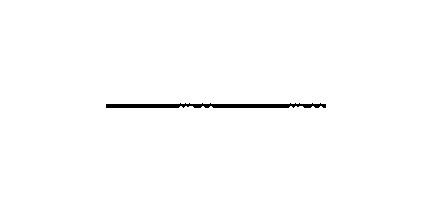
\includegraphics[width=3cm,height=3cm]{identity.png} 
\end{center}

\end{tcolorbox}
\end{center}


%LEAN: first triangle identity of the product-hom adjunction
\begin{center}
\begin{tcolorbox}[width=5in,colback={white},title={\begin{center}\texttt{Lean \thelcounter} \addtocounter{lcounter}{1}  \end{center}},colbacktitle=Blue,coltitle=black]
\begin{minted}[breaklines, escapeinside=||]{lean}

-- first triangle identity of the product-hom adjunction
/-
-/

\end{minted}%
\end{tcolorbox}
\end{center}


%LEAN: 
\begin{center}
\begin{tcolorbox}[width=5in,colback={white},title={\begin{center}\texttt{Graphic} \addtocounter{lcounter}{1}  \end{center}},colbacktitle=Yellow,coltitle=black]

\begin{center}
\includegraphics[width=8cm,height=8cm]{secondtriangle.png} \\
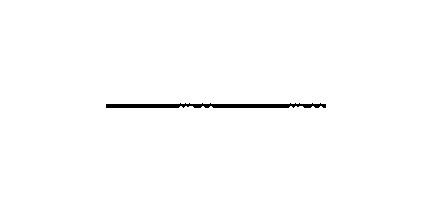
\includegraphics[width=3cm,height=3cm]{identity.png} 
\end{center}

\end{tcolorbox}
\end{center}

\section{\texttt{Prd X, τ, Δ}} %(1.5 days tops)

n-dimensional coordinates (arrays) are an ordinary construction, but we would do well to take careful note of its properties. The cartesian product $\texttt{X × Y}$ records the information of two mathematical objects at once in the way that $\texttt{x : X}$ and $\texttt{y : Y}$ can be recovered from the pair $\texttt{p : X} × \texttt{Y := (x, y)}$ as \texttt{x = p.fst}$ and $\texttt{y = p.snd}$. Above all, we might notice two particular other features which stand out about the cartesian product most: the terminal map $\texttt{τ : X → ⊛}$, which sends all elements of $\texttt{X}$ to the only element of ⊛, and the diagonal map: $\texttt{Δ : X → X}$ × $\texttt{X}$, λ $\texttt{(x : X) => (x, x)}$. These two maps and their properties reflect the so called $\textit{comonadicity}$ of cartesian product. Cartesian coordinates, while arising from the simple effort to combine pieces of information into array, already features the idiosyncracy of the diagonal and terminal maps.\\

%LEAN: Construction of the counit for product with X
\begin{center}
\begin{tcolorbox}[width=5in,colback={white},title={\begin{center}\texttt{Lean \thelcounter} \addtocounter{lcounter}{1}  \end{center}},colbacktitle=Blue,coltitle=black]
\begin{minted}[breaklines, escapeinside=||]{lean}

-- ε : X × Y ➞ Y
def Term (X : category) : (Prd X) ⇨ (𝟭 Cat) := sorry
notation "ε" => Term

\end{minted}%
\end{tcolorbox}
\end{center}

\begin{center}
\begin{tcolorbox}[width=5in,colback={white},title={\begin{center}\texttt{Graphic} \addtocounter{lcounter}{1}  \end{center}},colbacktitle=Yellow,coltitle=black]

Graphic for the counit of the Prd

\end{tcolorbox}
\end{center}

%LEAN: Construction of the comultiplication for product with X
\begin{center}
\begin{tcolorbox}[width=5in,colback={white},title={\begin{center}\texttt{Lean \thelcounter} \addtocounter{lcounter}{1}  \end{center}},colbacktitle=Blue,coltitle=black]
\begin{minted}[breaklines, escapeinside=||]{lean}

-- Δ : X × Y ➞ X × X × Y
def Diag (X : category) : (Prd X) ⇨ ((Prd X) • (Prd X)) := sorry

\end{minted}%
\end{tcolorbox}
\end{center}


%LEAN: 
\begin{center}
\begin{tcolorbox}[width=5in,colback={white},title={\begin{center}\texttt{Lean \thelcounter} \addtocounter{lcounter}{1}  \end{center}},colbacktitle=Blue,coltitle=black]
\begin{minted}[breaklines, escapeinside=||]{lean}

-- notation for the comultiplication for product with X
notation "Δ" => Diag

\end{minted}%
\end{tcolorbox}
\end{center}



\begin{center}
\begin{tcolorbox}[width=5in,colback={white},title={\begin{center}\texttt{Graphic} \addtocounter{lcounter}{1}  \end{center}},colbacktitle=Yellow,coltitle=black]

Graphic for the comultiplication of product with X

\end{tcolorbox}
\end{center}


%LEAN: proof of the first identity law of the comultiplication
\begin{center}
\begin{tcolorbox}[width=5in,colback={white},title={\begin{center}\texttt{Lean \thelcounter} \addtocounter{lcounter}{1}  \end{center}},colbacktitle=Blue,coltitle=black]
\begin{minted}[breaklines, escapeinside=||]{lean}

-- proof of the first identity law of the comultiplication
/-

-/

\end{minted}%
\end{tcolorbox}
\end{center}

\begin{center}
\begin{tcolorbox}[width=5in,colback={white},title={\begin{center} \texttt{Graphic} \addtocounter{lcounter}{1}  \end{center}},colbacktitle=Yellow,coltitle=black]

Graphic for the first identity law of comultiplication

\end{tcolorbox}
\end{center}


%LEAN: proof of the second identity law of the comultiplication
\begin{center}
\begin{tcolorbox}[width=5in,colback={white},title={\begin{center}\texttt{Lean \thelcounter} \addtocounter{lcounter}{1}  \end{center}},colbacktitle=Blue,coltitle=black]
\begin{minted}[breaklines, escapeinside=||]{lean}

-- proof of the second identity law of the comultiplication
/-

-/

\end{minted}%
\end{tcolorbox}
\end{center}

\begin{center}
\begin{tcolorbox}[width=5in,colback={white},title={\begin{center}\texttt{Graphic} \addtocounter{lcounter}{1}  \end{center}},colbacktitle=Yellow,coltitle=black]

Graphic for the second identity law of comultiplication

\end{tcolorbox}
\end{center}

%LEAN: proof of the coassociativity of the comultiplication
\begin{center}
\begin{tcolorbox}[width=5in,colback={white},title={\begin{center}\texttt{Lean \thelcounter} \addtocounter{lcounter}{1}  \end{center}},colbacktitle=Blue,coltitle=black]
\begin{minted}[breaklines, escapeinside=||]{lean}

-- proof of the coassociativity of the comultiplication
/-

-/

\end{minted}%
\end{tcolorbox}
\end{center}

\begin{center}
\begin{tcolorbox}[width=5in,colback={white},title={\begin{center}\texttt{Graphic} \addtocounter{lcounter}{1}  \end{center}},colbacktitle=Yellow,coltitle=black]

Graphic for coassociativity of the comultiplication

\end{tcolorbox}
\end{center}

\section{\texttt{Hom X, ι, μ}} %(1.5 days tops)


%LEAN: Construction of the unit for Hom X
\begin{center}
\begin{tcolorbox}[width=5in,colback={white},title={\begin{center}\texttt{Lean \thelcounter} \addtocounter{lcounter}{1}  \end{center}},colbacktitle=Blue,coltitle=black]
\begin{minted}[breaklines, escapeinside=||]{lean}

-- Construction of the unit for Hom X
def Const : (𝟭 Cat) ⇨ (Hom X) := sorry

\end{minted}%
\end{tcolorbox}
\end{center}


%LEAN: 
\begin{center}
\begin{tcolorbox}[width=5in,colback={white},title={\begin{center}\texttt{Lean \thelcounter} \addtocounter{lcounter}{1}  \end{center}},colbacktitle=Blue,coltitle=black]
\begin{minted}[breaklines, escapeinside=||]{lean}

-- notation 
/-

-/

\end{minted}%
\end{tcolorbox}
\end{center}


\begin{center}
\begin{tcolorbox}[width=5in,colback={white},title={\begin{center}\texttt{Graphic} \addtocounter{lcounter}{1}  \end{center}},colbacktitle=Yellow,coltitle=black]

Graphic for the unit for Hom X

\end{tcolorbox}
\end{center}


%LEAN: Construction of the multiplication for Hom X
\begin{center}
\begin{tcolorbox}[width=5in,colback={white},title={\begin{center}\texttt{Lean \thelcounter} \addtocounter{lcounter}{1}  \end{center}},colbacktitle=Blue,coltitle=black]
\begin{minted}[breaklines, escapeinside=||]{lean}

-- Construction of the multiplication for [X, -]
def double : (Hom X) ⇨ (Hom X) • (Hom X) := sorry

\end{minted}%
\end{tcolorbox}
\end{center}

\begin{center}
\begin{tcolorbox}[width=5in,colback={white},title={\begin{center}\texttt{Graphic} \addtocounter{lcounter}{1}  \end{center}},colbacktitle=Yellow,coltitle=black]

Graphic for the multiplication for Hom X

\end{tcolorbox}
\end{center}


%LEAN: proving the first unit law for the comonad Hom X
\begin{center}
\begin{tcolorbox}[width=5in,colback={white},title={\begin{center}\texttt{Lean \thelcounter} \addtocounter{lcounter}{1}  \end{center}},colbacktitle=Blue,coltitle=black]
\begin{minted}[breaklines, escapeinside=||]{lean}

-- 
/-

-/

\end{minted}%
\end{tcolorbox}
\end{center}


\begin{center}
\begin{tcolorbox}[width=5in,colback={white},title={\begin{center}\texttt{Graphic} \addtocounter{lcounter}{1}  \end{center}},colbacktitle=Yellow,coltitle=black]

Graphic for the first identity law of multiplication

\end{tcolorbox}
\end{center}


%LEAN: proving the second unit law for the comonad Hom X
\begin{center}
\begin{tcolorbox}[width=5in,colback={white},title={\begin{center}\texttt{Lean \thelcounter} \addtocounter{lcounter}{1}  \end{center}},colbacktitle=Blue,coltitle=black]
\begin{minted}[breaklines, escapeinside=||]{lean}

\end{minted}%
\end{tcolorbox}
\end{center}



\begin{center}
\begin{tcolorbox}[width=5in,colback={white},title={\begin{center}\texttt{Graphic} \addtocounter{lcounter}{1}  \end{center}},colbacktitle=Yellow,coltitle=black]

Graphic for the second identity law of multiplication

\end{tcolorbox}
\end{center}


%LEAN: proving associativity for the comonad Hom X
\begin{center}
\begin{tcolorbox}[width=5in,colback={white},title={\begin{center}\texttt{Lean \thelcounter} \addtocounter{lcounter}{1}  \end{center}},colbacktitle=Blue,coltitle=black]
\begin{minted}[breaklines, escapeinside=||]{lean}

-- proving associativity for the comonad (Hom X)
/-

-/

\end{minted}%
\end{tcolorbox}
\end{center}


\begin{center}
\begin{tcolorbox}[width=5in,colback={white},title={\begin{center}\texttt{Graphic} \addtocounter{lcounter}{1}  \end{center}},colbacktitle=Yellow,coltitle=black]

Graphic for associativity of the comultiplication

\end{tcolorbox}
\end{center}

\section{\texttt{(Prd X) • (Prd Y) ≅ (Prd Y) • (Prd X)}}%(1 day tops)


%LEAN: the twist map (X × -) • (Y × -) vs. (Y × -) • (X × -)
\begin{center}
\begin{tcolorbox}[width=5in,colback={white},title={\begin{center}\texttt{Lean \thelcounter \label{proof of the commutativity of categorical Prd}} \addtocounter{lcounter}{1}  \end{center}},colbacktitle=Blue,coltitle=black] 
\begin{minted}[breaklines, escapeinside=||]{lean}

-- proof of the commutativity of categorical Prd
def Tw₁ (C : category) (D : category) : ((Prd C) • (Prd D)) ⇨ ((Prd D) • (Prd C)) := sorry

\end{minted}%
\end{tcolorbox}
\end{center}


%LEAN: notation for the twist
\begin{center}
\begin{tcolorbox}[width=5in,colback={white},title={\begin{center}\texttt{Lean \thelcounter} \addtocounter{lcounter}{1}  \end{center}},colbacktitle=Blue,coltitle=black]
\begin{minted}[breaklines, escapeinside=||]{lean}

-- notation "τ₁" => Tw₁

\end{minted}%
\end{tcolorbox}
\end{center}



\begin{center}
\begin{tcolorbox}[width=5in,colback={white},title={\begin{center}\texttt{Graphic} \addtocounter{lcounter}{1}  \end{center}},colbacktitle=Yellow,coltitle=black]

\begin{center}
\includegraphics[width=4cm,height=4cm]{lbraid.png}
\end{center}

\end{tcolorbox}
\end{center}


%LEAN: proving that the twist map is its own inverse
\begin{center}
\begin{tcolorbox}[width=5in,colback={white},title={\begin{center}\texttt{Lean \thelcounter \label{proof of the commutativity of categorical Prd}} \addtocounter{lcounter}{1}  \end{center}},colbacktitle=Blue,coltitle=black] 
\begin{minted}[breaklines, escapeinside=||]{lean}

-- proving that the twist map is its own inverse
-- def (C : category) (D : category) : (τ ∘ τ = (Idn (C ⨯ D))) := sorry

\end{minted}%
\end{tcolorbox}
\end{center}

\begin{center}
\begin{tcolorbox}[width=5in,colback={white},title={\begin{center}\texttt{Graphic} \addtocounter{lcounter}{1}  \end{center}},colbacktitle=Yellow,coltitle=black]

\begin{center}
\includegraphics[width=6cm,height=4cm]{doubletwist.png}
\end{center}

\end{tcolorbox}
\end{center}


\section{\texttt{(Hom X) • (Hom Y) ≅ (Hom Y) • (Hom X)}} %(1 day tops)


%LEAN: defining the twist map (Hom X) • (Hom Y) ≅ (Hom Y) • (Hom X)
\begin{center}
\begin{tcolorbox}[width=5in,colback={white},title={\begin{center}\texttt{Lean \thelcounter \label{proof of the commutativity of categorical Prd}} \addtocounter{lcounter}{1}  \end{center}},colbacktitle=Blue,coltitle=black] 
\begin{minted}[breaklines, escapeinside=||]{lean}

-- defining the twist map (Hom X) • (Hom Y) ≅ (Hom Y) • (Hom X)
def Tw₂ (C : category) (D : category) : ((Hom C) • (Hom D)) ⇨ ((Hom D) • (Hom C)) := sorry
-- notation "τ₂" => Twist

\end{minted}%
\end{tcolorbox}
\end{center}

\begin{center}
\begin{tcolorbox}[width=5in,colback={white},title={\begin{center} Graphic \addtocounter{lcounter}{1}  \end{center}},colbacktitle=Yellow,coltitle=black]

\begin{center}
\includegraphics[width=4cm,height=4cm]{lbraid.png}
\end{center}

\end{tcolorbox}
\end{center}

%LEAN: proof that the twist map is its own inverse
\begin{center}
\begin{tcolorbox}[width=5in,colback={white},title={\begin{center}\texttt{Lean \thelcounter \label{proof of the commutativity of categorical Prd}} \addtocounter{lcounter}{1}  \end{center}},colbacktitle=Blue,coltitle=black] 
\begin{minted}[breaklines, escapeinside=||]{lean}

-- proof that the twist map is its own inverse
-- def (C : category) (D : category) : (τ ∘ τ = (Idn (C ⨯ D))) := sorry

\end{minted}%
\end{tcolorbox}
\end{center}

\begin{center}
\begin{tcolorbox}[width=5in,colback={white},title={\begin{center}\texttt{Graphic} \addtocounter{lcounter}{1}  \end{center}},colbacktitle=Yellow,coltitle=black]

\begin{center}
\includegraphics[width=6cm,height=4cm]{doubletwist.png}
\end{center}

\end{tcolorbox}
\end{center}

\section{\texttt{⊛}} %(1 day tops)

\begin{enumerate}
\item Defining the category ⊛
\item Notation for the category ⊛
\end{enumerate}


%LEAN: defining the category ⊛
\begin{center}
\begin{tcolorbox}[width=5in,colback={white},title={\begin{center}\texttt{Lean \thelcounter} \addtocounter{lcounter}{1}  \end{center}},colbacktitle=Blue,coltitle=black]
\begin{minted}[breaklines, escapeinside=||]{lean}

-- defining the category ⊛
def PntObj : Type := Unit
def PntHom (_ : PntObj) (_ : PntObj) : Type := Unit
def PntIdn (X : PntObj) : PntHom X X := Unit.unit
def PntCmp (X : PntObj) (Y : PntObj) (Z : PntObj) (_ : PntHom X Y) (_ : PntHom Y Z) : PntHom X Z := Unit.unit
def PntId₁ (X : PntObj) (Y : PntObj) (f : PntHom X Y) : PntCmp X Y Y f (PntIdn Y) = f := sorry
def PntId₂ (X : PntObj) (Y : PntObj) (f : PntHom X Y) : PntCmp X X Y (PntIdn X) f = f := sorry
def PntAss (W : PntObj) (X : PntObj) (Y : PntObj) (Z : PntObj) (f : PntHom W X) (g : PntHom X Y) (h : PntHom Y Z) : PntCmp W Y Z (PntCmp W X Y f g) h = PntCmp W X Z f (PntCmp X Y Z g h) := sorry
def Pnt : category := {Obj := PntObj, Hom := PntHom, Idn := PntIdn, Cmp := PntCmp, Id₁ := PntId₁, Id₂ := PntId₂, Ass := PntAss}

\end{minted}%
\end{tcolorbox}
\end{center}


%LEAN: notation for the category ⊛
\begin{center}
\begin{tcolorbox}[width=5in,colback={white},title={\begin{center}\texttt{Lean \thelcounter} \addtocounter{lcounter}{1}  \end{center}},colbacktitle=Green,coltitle=black]
\begin{minted}[breaklines, escapeinside=||]{lean}

-- notation for the category ⊛
notation "⊛" => Pnt

\end{minted}%
\end{tcolorbox}
\end{center}


\section{\texttt{Prd ⊛ ≅ 𝟭 Cat}} %(1 day tops)

\begin{enumerate}
\item Proving that (Prd ⊛) ≅ Idn
\begin{enumerate}
\item defining (Prd ⊛) ⇨ (𝟭 Cat)
\item defining (𝟭 Cat) ⇨ (Prd ⊛)
\item Proving the first inverse law for (Prd ⊛) ⇨ (𝟭 Cat) and (𝟭 Cat) ⇨ (Prd ⊛)
\item Proving the second inverse law for (Prd ⊛) ⇨ (𝟭 Cat) and (𝟭 Cat) ⇨ (Prd ⊛)
\end{enumerate}
\end{enumerate}

%LEAN: proving that (Prd ⊛) ≅ (𝟭 Cat)
\begin{center}
\begin{tcolorbox}[width=5in,colback={white},title={\begin{center}\texttt{Lean \thelcounter} \addtocounter{lcounter}{1}  \end{center}},colbacktitle=Blue,coltitle=black]
\begin{minted}[breaklines, escapeinside=||]{lean}

-- defining (Prd ⊛) ⇨ (𝟭 Cat)

\end{minted}%
\end{tcolorbox}
\end{center}

%LEAN: 
\begin{center}
\begin{tcolorbox}[width=5in,colback={white},title={\begin{center}\texttt{Lean \thelcounter} \addtocounter{lcounter}{1}  \end{center}},colbacktitle=Blue,coltitle=black]
\begin{minted}[breaklines, escapeinside=||]{lean}

-- defining (𝟭 Cat) ⇨ (Prd ⊛)

\end{minted}%
\end{tcolorbox}
\end{center}

%LEAN: 
\begin{center}
\begin{tcolorbox}[width=5in,colback={white},title={\begin{center}\texttt{Lean \thelcounter} \addtocounter{lcounter}{1}  \end{center}},colbacktitle=Blue,coltitle=black]
\begin{minted}[breaklines, escapeinside=||]{lean}

-- proving the first inverse identity

\end{minted}%
\end{tcolorbox}
\end{center}


%LEAN: 
\begin{center}
\begin{tcolorbox}[width=5in,colback={white},title={\begin{center}\texttt{Lean \thelcounter} \addtocounter{lcounter}{1}  \end{center}},colbacktitle=Blue,coltitle=black]
\begin{minted}[breaklines, escapeinside=||]{lean}

-- proving the second inverse identity

\end{minted}%
\end{tcolorbox}
\end{center}


\section{\texttt{Hom ⊛ ≅ 𝟭 Cat}} %(1 day tops)

\begin{enumerate}
\item Proving that \texttt{Hom ⊛ ≅ Idn}
\begin{enumerate}
\item Defining (Hom ⊛) ⇨ (𝟙 Cat)
\item Defining (𝟙 Cat) ⇨ (Hom ⊛)
\item Proving the first inverse law for (Hom ⊛) ⇨ (𝟙 Cat) and (𝟙 Cat) ⇨ (Hom ⊛)
\item Proving the second inverse law for (Hom ⊛) ⇨ (𝟙 Cat) and (𝟙 Cat) ⇨ (Hom ⊛)
\end{enumerate}
\end{enumerate}

Our next goal is to prove that Hom ⊛ is naturally isomorphic to $\texttt{𝟭 Cat}$. 

%LEAN: proving that (Hom ⊛) ≅ Idn
\begin{center}
\begin{tcolorbox}[width=5in,colback={white},title={\begin{center}\texttt{Lean \thelcounter} \addtocounter{lcounter}{1}  \end{center}},colbacktitle=Blue,coltitle=black]
\begin{minted}[breaklines, escapeinside=||]{lean}

-- defining (Hom ⊛) ⇨ (𝟭 Cat)
-- def IdnHomObj (C : category) : Hom ⊛ C 
-- def IdnHomHom 
-- def IdnHomIdn
-- def IdnHomCmp

\end{minted}%
\end{tcolorbox}
\end{center}


%LEAN: 
\begin{center}
\begin{tcolorbox}[width=5in,colback={white},title={\begin{center}\texttt{Lean \thelcounter} \addtocounter{lcounter}{1}  \end{center}},colbacktitle=Blue,coltitle=black]
\begin{minted}[breaklines, escapeinside=||]{lean}

-- defining (𝟭 Cat) ⇨ (Hom ⊛)
-- def IdnHom
-- def 
-- def 
-- def Idn

\end{minted}%
\end{tcolorbox}
\end{center}

%LEAN: 
\begin{center}
\begin{tcolorbox}[width=5in,colback={white},title={\begin{center}\texttt{Lean \thelcounter} \addtocounter{lcounter}{1}  \end{center}},colbacktitle=Blue,coltitle=black]
\begin{minted}[breaklines, escapeinside=||]{lean}

-- proving the first inverse identity

\end{minted}%
\end{tcolorbox}
\end{center}


%LEAN: 
\begin{center}
\begin{tcolorbox}[width=5in,colback={white},title={\begin{center}\texttt{Lean \thelcounter} \addtocounter{lcounter}{1}  \end{center}},colbacktitle=Blue,coltitle=black]
\begin{minted}[breaklines, escapeinside=||]{lean}

-- proving the second inverse identity
-- def Hom ⊛ ≅ X

\end{minted}%
\end{tcolorbox}
\end{center}


\section{Fox's Theorem} % 3 days tops


%LEAN: Defining the Prd of maps one way
\begin{center}
\begin{tcolorbox}[width=5in,colback={white},title={\begin{center}\texttt{Lean \thelcounter} \addtocounter{lcounter}{1}  \end{center}},colbacktitle=Blue,coltitle=black]
\begin{minted}[breaklines, escapeinside=||]{lean}

-- Defining the Prd F × G of two Hom one way
def FunPrd₁ {C₁ : category} {C₂ : category} {D₁ : category} {D₂ : category} (F : C₁ ➞ C₂) (G : D₁ ➞ D₂) : (PrdObj C₁ D₁) ➞ (PrdObj C₂ D₂) := sorry

\end{minted}%
\end{tcolorbox}
\end{center}


\begin{center}
\begin{tcolorbox}[width=5in,colback={white},title={\begin{center} Graphic \addtocounter{lcounter}{1}  \end{center}},colbacktitle=Yellow,coltitle=black]

Graphic for the Prd of Hom

\end{tcolorbox}
\end{center}


%LEAN: Defining the Prd F × G another way
\begin{center}
\begin{tcolorbox}[width=5in,colback={white},title={\begin{center}\texttt{Lean \thelcounter} \addtocounter{lcounter}{1}  \end{center}},colbacktitle=Blue,coltitle=black]
\begin{minted}[breaklines, escapeinside=||]{lean}

-- Defining the Prd F × G of two Hom the other way
def FunPrd₂ {C₁ : category} {C₂ : category} {D₁ : category} {D₂ : category} (F : C₁ ➞ C₂) (G : D₁ ➞ D₂) : (PrdObj C₁ D₁) ➞ (PrdObj C₂ D₂) := sorry

\end{minted}%
\end{tcolorbox}
\end{center}

\begin{center}
\begin{tcolorbox}[width=5in,colback={white},title={\begin{center} Graphic \addtocounter{lcounter}{1}  \end{center}},colbacktitle=Yellow,coltitle=black]

Graphic for the Prd of Hom 

\end{tcolorbox}
\end{center}


%LEAN: Equivalence of the two ways
\begin{center}
\begin{tcolorbox}[width=5in,colback={white},title={\begin{center}\texttt{Lean \thelcounter} \addtocounter{lcounter}{1}  \end{center}},colbacktitle=Blue,coltitle=black]
\begin{minted}[breaklines, escapeinside=||]{lean}

-- Showing that the two Prds are equal
theorem FunPrdEqn {C₁ : category} {C₂ : category} {D₁ : category} {D₂ : category} (F : C₁ ➞ C₂) (G : D₁ ➞ D₂) : FunPrd₁ F G = FunPrd₂ F G := sorry

\end{minted}%
\end{tcolorbox}
\end{center}

%LEAN: notation for the functor Prd
\begin{center}
\begin{tcolorbox}[width=5in,colback={white},title={\begin{center}\texttt{Lean \thelcounter} \addtocounter{lcounter}{1}  \end{center}},colbacktitle=Blue,coltitle=black]
\begin{minted}[breaklines, escapeinside=||]{lean}

-- notation for the functor Prd
notation F "⨯" G => FunPrd₁ F G

\end{minted}%
\end{tcolorbox}
\end{center}


%LEAN: Defining the canonical map in the universal property of Prd 
\begin{center}
\begin{tcolorbox}[width=5in,colback={white},title={\begin{center}\texttt{Lean \thelcounter} \addtocounter{lcounter}{1}  \end{center}},colbacktitle=Blue,coltitle=black]
\begin{minted}[breaklines, escapeinside=||]{lean}

-- Defining the canonical map in the universal property of Prd
-- def 

\end{minted}%
\end{tcolorbox}
\end{center}


\begin{center}
\begin{tcolorbox}[width=5in,colback={white},title={\begin{center} Graphic \addtocounter{lcounter}{1}  \end{center}},colbacktitle=Yellow,coltitle=black]

Graphic for the equivalence

\end{tcolorbox}
\end{center}


%LEAN: Proving the uniqueness of the canonical map in the universal property of Prd
\begin{center}
\begin{tcolorbox}[width=5in,colback={white},title={\begin{center}\texttt{Lean \thelcounter} \addtocounter{lcounter}{1}  \end{center}},colbacktitle=Blue,coltitle=black]
\begin{minted}[breaklines, escapeinside=||]{lean}

-- Proving the uniqueness of the canonical map in the universal property of Prd
/-
theorem (uniqueness of the canonical map)
-/

\end{minted}%
\end{tcolorbox}
\end{center}


\begin{center}
\begin{tcolorbox}[width=5in,colback={white},title={\begin{center} Graphic \addtocounter{lcounter}{1}  \end{center}},colbacktitle=Yellow,coltitle=black]

Graphic for the proof of Fox's theorem

\end{tcolorbox}
\end{center}



%LEAN: 
\begin{center}
\begin{tcolorbox}[width=5in,colback={white},title={\begin{center}\texttt{Lean \thelcounter} \addtocounter{lcounter}{1}  \end{center}},colbacktitle=Blue,coltitle=black]
\begin{minted}[breaklines, escapeinside=||]{lean}

-- 
/-

-/

\end{minted}%
\end{tcolorbox}
\end{center}




%PYTHON:
\begin{center}
\begin{tcolorbox}[width=5in,colback={white},title={\begin{center}\texttt{Python \thepcounter} \addtocounter{pcounter}{1}  \end{center}},colbacktitle=Red,coltitle=black]
\begin{minted}[breaklines, escapeinside=||]{python}


from PIL import Image, ImageDraw
from PIL import ImageFont
from math import *

\end{minted}%
\end{tcolorbox}
\end{center}

%PYTHON:
\begin{center}
\begin{tcolorbox}[width=5in,colback={white},title={\begin{center}\texttt{Python \thepcounter} \addtocounter{pcounter}{1}  \end{center}},colbacktitle=Red,coltitle=black]
\begin{minted}[breaklines, escapeinside=||]{python}

def index(list):
    return range(len(list))

\end{minted}%
\end{tcolorbox}
\end{center}

%PYTHON:
\begin{center}
\begin{tcolorbox}[width=5in,colback={white},title={\begin{center}\texttt{Python \thepcounter} \addtocounter{pcounter}{1}  \end{center}},colbacktitle=Red,coltitle=black]
\begin{minted}[breaklines, escapeinside=||]{python}

class vector:
    def __init__(self, entries):
        self.entries = entries
        self.length = len(entries)

    def __getitem__(self, i):
        return self.entries[i]

    def __add__(self, other):
        entries = []
        for i in range(len(self.entries)):
            entries.append(self[i] + other[i])
        return vector(entries)

    def __rmul__(self, a):
        entries = []
        for i in range(len(self.entries)):
            entries.append(a*self[i])
        return vector(entries)

    def height(self):
        return self.entries[1] - self.entries[0]

    def average(self):
        (1/float(len(self.entries)))*sum([self.entries])

    def print(self):
        print(self.entries)


\end{minted}%
\end{tcolorbox}
\end{center}

%PYTHON:
\begin{center}
\begin{tcolorbox}[width=5in,colback={white},title={\begin{center}\texttt{Python \thepcounter} \addtocounter{pcounter}{1}  \end{center}},colbacktitle=Red,coltitle=black]
\begin{minted}[breaklines, escapeinside=||]{python}

def exp(theta):
    return vector([cos(theta), sin(theta)])

\end{minted}%
\end{tcolorbox}
\end{center}

%PYTHON:
\begin{center}
\begin{tcolorbox}[width=5in,colback={white},title={\begin{center}\texttt{Python \thepcounter} \addtocounter{pcounter}{1}  \end{center}},colbacktitle=Red,coltitle=black]
\begin{minted}[breaklines, escapeinside=||]{python}


def interpolation(t):
    if 0 <= t and t <= 0.5:
        return 0.5 - sqrt(0.25-t*t)
    if 0.5 < t <= 1:
        s = 1-t
        return 0.5 + sqrt(0.25-s*s)
    return (-2.77333)*t*t*t + 4.16*t*t + (-0.386667)*t

\end{minted}%
\end{tcolorbox}
\end{center}

%PYTHON:
\begin{center}
\begin{tcolorbox}[width=5in,colback={white},title={\begin{center}\texttt{Python \thepcounter} \addtocounter{pcounter}{1}  \end{center}},colbacktitle=Red,coltitle=black]
\begin{minted}[breaklines, escapeinside=||]{python}


def curve(coordinates, border):
    for counter in range(len(coordinates) - 1):
        a = coordinates[counter][0]
        b = coordinates[counter+1][0]
        i = coordinates[counter][1]
        j = coordinates[counter+1][1]
        draw.line((j, b, i, a), fill=(256, 256, 256), width=12) 
        draw.line((j, b, i, a), fill=(0, 0, 0), width=4)
    image.save('test.png')      

\end{minted}%
\end{tcolorbox}
\end{center}

%PYTHON:
\begin{center}
\begin{tcolorbox}[width=5in,colback={white},title={\begin{center}\texttt{Python \thepcounter} \addtocounter{pcounter}{1}  \end{center}},colbacktitle=Red,coltitle=black]
\begin{minted}[breaklines, escapeinside=||]{python}

def squiggle(v1, v2, border):
    coordinates = []
    l = 100
    for r in range(l):
        t = float(r)/l
        s = interpolation(t)
        x = s*v1[0] + (1-s)*v2[0]
        y = t*v1[1] + (1-t)*v2[1]
        coordinates.append([x, y])
    curve(coordinates, border)

\end{minted}%
\end{tcolorbox}
\end{center}

%PYTHON:
\begin{center}
\begin{tcolorbox}[width=5in,colback={white},title={\begin{center}\texttt{Python \thepcounter} \addtocounter{pcounter}{1}  \end{center}},colbacktitle=Red,coltitle=black]
\begin{minted}[breaklines, escapeinside=||]{python}

def arc(v, r, theta1, theta2, u, border):
    n = floor((theta2 - theta1)*300)
    coordinates = []
    for i in range(n):
        t = float(float(i) * (theta2 - theta1)) / float(n)
        if u ==0:
            w = v +(-1)* r*exp(t)
        if u == 1:
            w = v + r*exp(t)          
        coordinates.append(w)
    curve(coordinates, border)

\end{minted}%
\end{tcolorbox}
\end{center}

%PYTHON:
\begin{center}
\begin{tcolorbox}[width=5in,colback={white},title={\begin{center}\texttt{Python \thepcounter} \addtocounter{pcounter}{1}  \end{center}},colbacktitle=Red,coltitle=black]
\begin{minted}[breaklines, escapeinside=||]{python}

def bubble(v, color):
    draw.ellipse((v[1]-13, v[0]-13, v[1]+13, v[0]+13), fill = (0,0 ,0))
    draw.ellipse((v[1]-10, v[0]-10, v[1]+10, v[0]+10), fill = color)

\end{minted}%
\end{tcolorbox}
\end{center}

%PYTHON:
\begin{center}
\begin{tcolorbox}[width=5in,colback={white},title={\begin{center}\texttt{Python \thepcounter} \addtocounter{pcounter}{1}  \end{center}},colbacktitle=Red,coltitle=black]
\begin{minted}[breaklines, escapeinside=||]{python}

class cell:
    def __init__(self, entries, border, bubble, color):
        self.symbol = None
        self.entries = entries
        self.border = border
        self.x1    = entries[0]
        self.y11   = entries[1]
        self.y12   = entries[2]
        self.x2    = entries[0] +1
        self.y21   = entries[3]
        self.y22   = entries[4]
        self.y1 = self.y12 - self.y11
        self.y2 = self.y22 - self.y21
        self.width = 1
        self.bubble = bubble
        self.color = color

    def print(self):
        print("x1: ", self.x1)
        print("y11: ", self.y11)
        print("y12: ", self.y12)
        print("x2: ", self.x2)
        print("y21: ", self.y21)
        print("y22: ", self.y22)

    def copy(self):
        x1 = self.x1
        y11 = self.y11
        y12 = self.y12
        y21 = self.y21
        y22 = self.y22
        border = self.border
        bubble = self.bubble
        color = self.color
        return cell([x1, y11, y12, y21, y22], border, bubble, color)

\end{minted}%
\end{tcolorbox}
\end{center}

%PYTHON:
\begin{center}
\begin{tcolorbox}[width=5in,colback={white},title={\begin{center}\texttt{Python \thepcounter} \addtocounter{pcounter}{1}  \end{center}},colbacktitle=Red,coltitle=black]
\begin{minted}[breaklines, escapeinside=||]{python}

def copy_cell(l):
    cells = []
    for c in l:
        d = c.copy()
        cells.append(d)
    return cells

\end{minted}%
\end{tcolorbox}
\end{center}

%PYTHON:
\begin{center}
\begin{tcolorbox}[width=5in,colback={white},title={\begin{center}\texttt{Python \thepcounter} \addtocounter{pcounter}{1}  \end{center}},colbacktitle=Red,coltitle=black]
\begin{minted}[breaklines, escapeinside=||]{python}

def xshift(c, t):
    x1 = c.x1 + t
    x2 = c.x2 + t
    y11 = c.y11
    y12 = c.y12
    y21 = c.y21
    y22 = c.y22
    border = c.border
    bubble = c.bubble
    color = c.color
    return cell([x1, y11, y12, y21, y22], border, bubble, color)

\end{minted}%
\end{tcolorbox}
\end{center}

%PYTHON:
\begin{center}
\begin{tcolorbox}[width=5in,colback={white},title={\begin{center}\texttt{Python \thepcounter} \addtocounter{pcounter}{1}  \end{center}},colbacktitle=Red,coltitle=black]
\begin{minted}[breaklines, escapeinside=||]{python}

def yshift(c, y1, y2):
    y11 = c.y11 + y1
    y12 = c.y12 + y1
    y21 = c.y21 + y2
    y22 = c.y22 + y2
    x1 = c.x1
    border = c.border
    bubble = c.bubble
    color = c.color
    return cell([x1, y11, y12, y21, y22], border, bubble, color)

\end{minted}%
\end{tcolorbox}
\end{center}

%PYTHON:
\begin{center}
\begin{tcolorbox}[width=5in,colback={white},title={\begin{center}\texttt{Python \thepcounter} \addtocounter{pcounter}{1}  \end{center}},colbacktitle=Red,coltitle=black]
\begin{minted}[breaklines, escapeinside=||]{python}

class diagram:
    def __init__(self, heights, cells):
        self.color = color
        self.heights = heights
        self.width = len(heights)
        self.height = 0
        for h in self.heights:
            if h > self.height:
                self.height = h
        self.height = self.height
        self.cells = cells

\end{minted}%
\end{tcolorbox}
\end{center}

%PYTHON:
\begin{center}
\begin{tcolorbox}[width=5in,colback={white},title={\begin{center}\texttt{Python \thepcounter} \addtocounter{pcounter}{1}  \end{center}},colbacktitle=Red,coltitle=black]
\begin{minted}[breaklines, escapeinside=||]{python}

    def __mul__(self, other):
        assert self.heights[-1] == other.heights[0]

        heights = self.heights[0:-1].copy() + other.heights.copy()

        cells = copy_cell(self.cells)
        for cell in copy_cell(other.cells):
            cells.append(xshift(cell, self.width - 1))

        return diagram(heights, cells)

\end{minted}%
\end{tcolorbox}
\end{center}

%PYTHON:
\begin{center}
\begin{tcolorbox}[width=5in,colback={white},title={\begin{center}\texttt{Python \thepcounter} \addtocounter{pcounter}{1}  \end{center}},colbacktitle=Red,coltitle=black]
\begin{minted}[breaklines, escapeinside=||]{python}

    def __add__(self, other):
        cells = self.cells.copy()
        for i in range(len(other.cells)):
            x1 = other.cells[i].x1
            x2 = other.cells[i].x2
            h1 = self.heights[x1]
            h2 = self.heights[x2]
            cells.append(yshift(other.cells[i], h1, h2))
        p = len(self.heights)
        return diagram([self.heights[i] + other.heights[i] for i in range(p)], cells)

\end{minted}%
\end{tcolorbox}
\end{center}

%PYTHON:
\begin{center}
\begin{tcolorbox}[width=5in,colback={white},title={\begin{center}\texttt{Python \thepcounter} \addtocounter{pcounter}{1}  \end{center}},colbacktitle=Red,coltitle=black]
\begin{minted}[breaklines, escapeinside=||]{python}

    def coordinate(self, v, unit,  W, H):
        h = unit*self.heights[v[0]]
        w = unit*self.width
        x = unit*float(v[0])
        y = unit*float(v[1])
        a = H/2-h/2 + unit*v[1]
        b = W/2-w/2 + unit*v[0] + unit/2
        return vector([a, b])

\end{minted}%
\end{tcolorbox}
\end{center}

%PYTHON:
\begin{center}
\begin{tcolorbox}[width=5in,colback={white},title={\begin{center}\texttt{Python \thepcounter} \addtocounter{pcounter}{1}  \end{center}},colbacktitle=Red,coltitle=black]
\begin{minted}[breaklines, escapeinside=||]{python}

    def print(self, name, unit = 110, border = 0, radius = 10):
        file_name = name + ".png"
        global image
        W = unit*self.width + 100
        H = unit*self.height + 100
        image = Image.new('RGBA', (W, H), (256,256,256))
        global draw
        draw = ImageDraw.Draw(image)
        for cell in self.cells:
            v11 = self.coordinate(vector([cell.x1, cell.y11]), unit, W, H)
            v12 = self.coordinate(vector([cell.x2, cell.y21]), unit, W, H)
            v21 = self.coordinate(vector([cell.x1, cell.y12]), unit, W, H)
            v22 = self.coordinate(vector([cell.x2, cell.y22]), unit, W, H)
            m1 = (1/2)*(v11 + v21)
            m2 = (1/2)*(v12 + v22)
            o = (1/2)*(m1 + m2)

\end{minted}%
\end{tcolorbox}
\end{center}

%PYTHON:
\begin{center}
\begin{tcolorbox}[width=5in,colback={white},title={\begin{center}\texttt{Python \thepcounter} \addtocounter{pcounter}{1}  \end{center}},colbacktitle=Red,coltitle=black]
\begin{minted}[breaklines, escapeinside=||]{python}

            if cell.y1 == 0 and cell.y2 == 1:
                squiggle(m1, o, cell.border) 
                if cell.bubble == 1:
                    bubble(o, self.color)
                image.save(file_name)

\end{minted}%
\end{tcolorbox}
\end{center}

%PYTHON:
\begin{center}
\begin{tcolorbox}[width=5in,colback={white},title={\begin{center}\texttt{Python \thepcounter} \addtocounter{pcounter}{1}  \end{center}},colbacktitle=Red,coltitle=black]
\begin{minted}[breaklines, escapeinside=||]{python}

            if cell.y1 == 0 and cell.y2 == 2:
                arc(m2, unit/2, -0.05, pi+0.05, 0, cell.border)
                if cell.bubble == 1:
                    bubble(o+ vector([-unit/2, 0]), cell.color)
                image.save(file_name)

\end{minted}%
\end{tcolorbox}
\end{center}

%PYTHON:
\begin{center}
\begin{tcolorbox}[width=5in,colback={white},title={\begin{center}\texttt{Python \thepcounter} \addtocounter{pcounter}{1}  \end{center}},colbacktitle=Red,coltitle=black]
\begin{minted}[breaklines, escapeinside=||]{python}

            if cell.y1 == 1 and cell.y2 == 0:
                squiggle(o, m2, cell.border)
                if cell.bubble == 1:
                    bubble(o, cell.color)
                image.save(file_name)

\end{minted}%
\end{tcolorbox}
\end{center}

%PYTHON:
\begin{center}
\begin{tcolorbox}[width=5in,colback={white},title={\begin{center}\texttt{Python \thepcounter} \addtocounter{pcounter}{1}  \end{center}},colbacktitle=Red,coltitle=black]
\begin{minted}[breaklines, escapeinside=||]{python}

            if cell.y1 == 1 and cell.y2 == 1:
                squiggle(m1, m2, cell.border)
                if cell.bubble == 1:
                    bubble(o, cell.color)
                image.save(file_name)

\end{minted}%
\end{tcolorbox}
\end{center}

%PYTHON:
\begin{center}
\begin{tcolorbox}[width=5in,colback={white},title={\begin{center}\texttt{Python \thepcounter} \addtocounter{pcounter}{1}  \end{center}},colbacktitle=Red,coltitle=black]
\begin{minted}[breaklines, escapeinside=||]{python}

            if cell.y1 == 1 and cell.y2 == 2:
                a = (1/4)*(3*v22 + v12)
                b = (1/4)*(v22 + 3*v12)
                squiggle(o, a, cell.border)
                squiggle(o, b, cell.border)
                squiggle(m1, o, cell.border)
                p = vector([o[0], o[1]])
                if cell.bubble == 1:
                    bubble(p, cell.color)
                image.save(file_name)

\end{minted}%
\end{tcolorbox}
\end{center}

%PYTHON:
\begin{center}
\begin{tcolorbox}[width=5in,colback={white},title={\begin{center}\texttt{Python \thepcounter} \addtocounter{pcounter}{1}  \end{center}},colbacktitle=Red,coltitle=black]
\begin{minted}[breaklines, escapeinside=||]{python}

            if cell.y1 == 2 and cell.y2 == 0:
                arc(m1, unit/2, -0.05, pi+0.05, 1, cell.border)
                if cell.bubble == 1:
                    bubble(o + vector([unit/2, 0]), cell.color)
                image.save(file_name)

\end{minted}%
\end{tcolorbox}
\end{center}

%PYTHON:
\begin{center}
\begin{tcolorbox}[width=5in,colback={white},title={\begin{center}\texttt{Python \thepcounter} \addtocounter{pcounter}{1}  \end{center}},colbacktitle=Red,coltitle=black]
\begin{minted}[breaklines, escapeinside=||]{python}

            if cell.y1 == 2 and cell.y2 == 1:
                a = (1/4)*(3*v21 + v11)
                b = (1/4)*(v21 + 3*v11)
                squiggle(a, o, cell.border)
                squiggle(b, o, cell.border)
                squiggle(o, m2, cell.border)
                p = vector([o[0], o[1]])
                if cell.bubble == 1:
                    bubble(p, cell.color)
                image.save(file_name)

\end{minted}%
\end{tcolorbox}
\end{center}

%PYTHON:
\begin{center}
\begin{tcolorbox}[width=5in,colback={white},title={\begin{center}\texttt{Python \thepcounter} \addtocounter{pcounter}{1}  \end{center}},colbacktitle=Red,coltitle=black]
\begin{minted}[breaklines, escapeinside=||]{python}

            if cell.y1 == 2 and cell.y2 == 2:
                w11 = (1/2)*(v11 + m1)
                w12 = (1/2)*(v12 + m2)
                w21 = (1/2)*(v21 + m1)
                w22 = (1/2)*(v22 + m2)
                if cell.border == 1:
                    squiggle(w12, w21, 1)
                    squiggle(w11, w22, 1)
                if cell.border == 2:
                    squiggle(w11, w22, 1)
                    squiggle(w12, w21, 1)
                if cell.bubble == 1:
                    bubble(o, cell.color)
                image.save(file_name)

\end{minted}%
\end{tcolorbox}
\end{center}

%PYTHON:
\begin{center}
\begin{tcolorbox}[width=5in,colback={white},title={\begin{center}\texttt{Python \thepcounter} \addtocounter{pcounter}{1}  \end{center}},colbacktitle=Red,coltitle=black]
\begin{minted}[breaklines, escapeinside=||]{python}

def make_cell(i, j, color =(0, 0, 0), border = 0, bubble =0):
    return diagram([i, j], [cell([0, 0, i, 0, j], border, bubble, color)])   

\end{minted}%
\end{tcolorbox}
\end{center}

%PYTHON:
\begin{center}
\begin{tcolorbox}[width=5in,colback={white},title={\begin{center}\texttt{Python \thepcounter} \addtocounter{pcounter}{1}  \end{center}},colbacktitle=Red,coltitle=black]
\begin{minted}[breaklines, escapeinside=||]{python}

blue = (102, 178, 255)
green = (0, 204, 102)
yellow = (250, 250, 50)
brown = (30, 150, 69)
color = blue

\end{minted}%
\end{tcolorbox}
\end{center}

%PYTHON:
\begin{center}
\begin{tcolorbox}[width=5in,colback={white},title={\begin{center}\texttt{Python \thepcounter} \addtocounter{pcounter}{1}  \end{center}},colbacktitle=Red,coltitle=black]
\begin{minted}[breaklines, escapeinside=||]{python}

counit = make_cell(2, 0, blue,1, 0)
unit = make_cell(0, 2, blue, 1, 0)
Unit = make_cell(0, 1, blue, 1, 0)
Counit = make_cell(1, 0, blue, 1, 0)
Multiplication = make_cell(2, 1, blue, 1, 0)
Comultiplication = make_cell(1, 2, blue, 1, 0)
IdF = make_cell(1, 1, blue, 1, 1)
IdG = make_cell(1, 1, blue, 1, 0)
identity = make_cell(1, 1, blue, 0, 0)
Ltriangle = (unit + IdG)*(IdF + counit)
Rtriangle = (IdG + unit)*(counit + IdF)
Lbraid = make_cell(2, 2, blue, 1, 0)
Rbraid = make_cell(2, 2, blue, 2, 0)
a1 = unit+identity+identity
a2 = identity + counit +identity
a3 = unit + identity+identity
a4 = identity + identity + counit
Multiplication.print("test10")

#To do:
#Make each cell have its own color
#Get each cell to have a plus or a minus sign
#Strings with a grade of color for permeable membranes
#Strings which are colored or which stand for terms





\end{minted}%
\end{tcolorbox}
\end{center}

\newpage
asdfasdfasdf
\includegraphics[width=1cm,height=1cm]{test10.png}
asdfasdf

\newpage
\ \


{
\Huge 
\begin{center}
\texttt{Chapter II: the (strict) twocategory of categories}
\end{center}
\thispagestyle{empty}
}

\ \\
\ \\
\ \\

{
\small
\begin{center}
\begin{tabular}{|l | l |} 
 \hline
 $\texttt{Section}$ & $\texttt{Description}$ \\
 \hline
 \hline
 \texttt{twocategory} &\ the (strict) twocategory structure \\
 \hline
 \texttt{Two} &\ the twocategory of categories \\
 \hline
 • &\ notation for horizontal composition \\
 \hline
\end{tabular}
\end{center}
}

\section{\texttt{twocategory}} % 1 day tops


%LEAN: definition of a (strict) twocategory
\begin{center}
\begin{tcolorbox}[width=5in,colback={white},title={\begin{center}\texttt{Lean \thelcounter} \addtocounter{lcounter}{1}  \end{center}},colbacktitle=Blue,coltitle=black]
\begin{minted}[breaklines, escapeinside=||]{lean}

-- definition of a (strict) twocategory
structure twocategory where
  TwoObj : Type
  TwoHom : TwoObj → TwoObj → category
  TwoIdn : (C : TwoObj) → ⊛ ➞ (TwoHom C C)
  TwoCmp : (C : TwoObj) → (D : TwoObj) → (E : TwoObj) → (PrdObj (TwoHom C D) (TwoHom D E)) ➞ (TwoHom C E)
--  TwoId₁ : (C : Obj) → (D : Obj) → (TwoCmp C D D) • ((Idn 1) ⨯ (𝟭 )) = 
--  TwoId₂ : (C : Obj) → (D : Obj) → (Cmp C C D) • ((Idn D) × 1) = 
--  Ass : (B : Obj) → (C : Obj) → (D : Obj) → (E : Obj) → (((Cmp B C E) • (FunPrd₁ (𝟭 (Hom B C)) (Cmp C D E))) = (Cmp B D E • (FunPrd₁ (Cmp B C D) (𝟭 (Hom D E)))))

\end{minted}%
\end{tcolorbox}
\end{center}


%LEAN: notation for a twocategory
\begin{center}
\begin{tcolorbox}[width=5in,colback={white},title={\begin{center}\texttt{Lean \thelcounter} \addtocounter{lcounter}{1}  \end{center}},colbacktitle=Blue,coltitle=black]
\begin{minted}[breaklines, escapeinside=||]{lean}

-- notation for a twocategory
/-

-/

\end{minted}%
\end{tcolorbox}
\end{center}


\section{\texttt{Two}} % 2 days tops

Next we define "categories", the (strict) twocategory of categories. We have already defined categories.Obj := category and categories.Hom := functor, so we may start by defining the Idn component:\\

%LEAN: defining categories.Idn.Obj
\begin{center}
\begin{tcolorbox}[width=5in,colback={white},title={\begin{center}\texttt{Lean \thelcounter} \addtocounter{lcounter}{1}  \end{center}},colbacktitle=Blue,coltitle=black]
\begin{minted}[breaklines, escapeinside=||]{lean}

-- defining categories.Idn.Obj
def TwoIdnObj (C : category) (_ : Unit) := Cat.Idn C

\end{minted}%
\end{tcolorbox}
\end{center}


%LEAN: defining the functor categories.Idn.Hom
\begin{center}
\begin{tcolorbox}[width=5in,colback={white},title={\begin{center}\texttt{Lean \thelcounter} \addtocounter{lcounter}{1}  \end{center}},colbacktitle=Blue,coltitle=black]
\begin{minted}[breaklines, escapeinside=||]{lean}

-- defining the functor categories.Idn.Hom on morphisms
def TwoIdnHom (C : category) (_ : Unit) (_ : Unit) (_: Unit) := (HomObj C C).Idn (Cat.Idn C)

\end{minted}%
\end{tcolorbox}
\end{center}


%LEAN: proving the identity law for the functor categoriIdn
\begin{center}
\begin{tcolorbox}[width=5in,colback={white},title={\begin{center}\texttt{Lean \thelcounter} \addtocounter{lcounter}{1}  \end{center}},colbacktitle=Blue,coltitle=black]
\begin{minted}[breaklines, escapeinside=||]{lean}

-- proving the identity law for the functor categories.TwoIdn
-- def TwoIdnIdn (C : category) (_ : Unit) (_ : Unit) (_: Unit) := (HomObj C C).Idn (Cat.Idn C)

\end{minted}%
\end{tcolorbox}
\end{center}


%LEAN: proving compositionality for the functor categories.TwoIdn
\begin{center}
\begin{tcolorbox}[width=5in,colback={white},title={\begin{center}\texttt{Lean \thelcounter} \addtocounter{lcounter}{1}  \end{center}},colbacktitle=Blue,coltitle=black]
\begin{minted}[breaklines, escapeinside=||]{lean}

-- proving compositionality for the functor categories.TwoIdn
-- def Two.Idn.Cmp (C : category) (_ : Unit) (_ : Unit) (_: Unit) := (HomObj C C).Idn (Cat.Idn C)

\end{minted}%
\end{tcolorbox}
\end{center}


%LEAN: defining categories.Idn
\begin{center}
\begin{tcolorbox}[width=5in,colback={white},title={\begin{center}\texttt{Lean \thelcounter} \addtocounter{lcounter}{1}  \end{center}},colbacktitle=Blue,coltitle=black]
\begin{minted}[breaklines, escapeinside=||]{lean}

-- def categories.Idn
def TwoIdn (C : category) : ⊛ ➞ (HomObj C C) := sorry

\end{minted}%
\end{tcolorbox}
\end{center}

Next we define Two.Cmp:\\

%LEAN: defining categories.Cmp.Obj
\begin{center}
\begin{tcolorbox}[width=5in,colback={white},title={\begin{center}\texttt{Lean \thelcounter} \addtocounter{lcounter}{1}  \end{center}},colbacktitle=Blue,coltitle=black]
\begin{minted}[breaklines, escapeinside=||]{lean}

--  defining Two.Cmp.Obj
/-
-/

\end{minted}%
\end{tcolorbox}
\end{center}


%LEAN: defining Two.Cmp.Hom
\begin{center}
\begin{tcolorbox}[width=5in,colback={white},title={\begin{center}\texttt{Lean \thelcounter} \addtocounter{lcounter}{1}  \end{center}},colbacktitle=Blue,coltitle=black]
\begin{minted}[breaklines, escapeinside=||]{lean}

--  defining Two.Cmp.Hom
/-
def TwoTwoHom (C : Obj) (D : Obj) (E : Obj)  : FG.1 FG.2
def TwoTwoHom (C : Obj) (D : Obj) (E : Obj) (f : ((Hom C D) ⨯ (Hom D E)).Hom )
def CatsHom (C : Obj) (D : Obj) (E : Obj) 
(F₁G₁ : ((Hom C D) ⨯ (Hom D E)).Obj) (F₂G₂ : ((Hom C D) ⨯ (Hom D E)).Obj)
-/


\end{minted}%
\end{tcolorbox}
\end{center}


%LEAN: proving the identity law equation for Two.TwoCmp
\begin{center}
\begin{tcolorbox}[width=5in,colback={white},title={\begin{center}\texttt{Lean \thelcounter} \addtocounter{lcounter}{1}  \end{center}},colbacktitle=Blue,coltitle=black]
\begin{minted}[breaklines, escapeinside=||]{lean}

-- proving the identity law equation for Two.TwoCmp
/-
def 
-/

\end{minted}%
\end{tcolorbox}
\end{center}


%LEAN: proving compositionality for the functor Two.Cmp
\begin{center}
\begin{tcolorbox}[width=5in,colback={white},title={\begin{center}\texttt{Lean \thelcounter} \addtocounter{lcounter}{1}  \end{center}},colbacktitle=Blue,coltitle=black]
\begin{minted}[breaklines, escapeinside=||]{lean}

-- proving compositionality for the functor Two.Cmp
-- def TwoCmpCmp : (C : category) → (D : category) → (E : category) → (PrdObj (HomObj C D) (HomObj D E)) ➞ (HomObj C E) := sorry

\end{minted}%
\end{tcolorbox}
\end{center}


%LEAN: defining Two.Cmp 
\begin{center}
\begin{tcolorbox}[width=5in,colback={white},title={\begin{center}\texttt{Lean \thelcounter} \addtocounter{lcounter}{1}  \end{center}},colbacktitle=Blue,coltitle=black]
\begin{minted}[breaklines, escapeinside=||]{lean}

--  Two.Cmp : (C : Obj) → (D : Obj) → (E : Obj) → (Hom C D) × (Hom D E) ➞ (Hom C E)    
def TwoCmp : (C : category) → (D : category) → (E : category) → (PrdObj (HomObj C D) (HomObj D E)) ➞ (HomObj C E) := sorry

\end{minted}%
\end{tcolorbox}
\end{center}

Now that we have constructed the first four constituents of the twocategory Two, we proceed to prove that they satisfy the three conditions Id₁, Id₂, and Ass:\\

%LEAN: defining Two.Id₁
\begin{center}
\begin{tcolorbox}[width=5in,colback={white},title={\begin{center}\texttt{Lean \thelcounter} \addtocounter{lcounter}{1}  \end{center}},colbacktitle=Blue,coltitle=black]
\begin{minted}[breaklines, escapeinside=||]{lean}

--  Id₁ : (C : Obj) → (D : Obj) → (Cats.Id₁)
/-
def TwoId₁ : (C : category) → (D : category) → (F : functor C D) → 
-/

\end{minted}%
\end{tcolorbox}
\end{center}


%LEAN: defining Two.Id₂
\begin{center}
\begin{tcolorbox}[width=5in,colback={white},title={\begin{center}\texttt{Lean \thelcounter} \addtocounter{lcounter}{1}  \end{center}},colbacktitle=Blue,coltitle=black]
\begin{minted}[breaklines, escapeinside=||]{lean}

--  Id₂ : (C : Obj) → (D : Obj) → (F : (Hom C D).Obj) → ...      (Cats.Id₁)
/-
def TwoId₂ : (C : category) → (D : category) → (F : functor C D) → 
-/

\end{minted}%
\end{tcolorbox}
\end{center}


%LEAN: proving Two.Ass
\begin{center}
\begin{tcolorbox}[width=5in,colback={white},title={\begin{center}\texttt{Lean \thelcounter} \addtocounter{lcounter}{1}  \end{center}},colbacktitle=Blue,coltitle=black]
\begin{minted}[breaklines, escapeinside=||]{lean}

-- proving associativity of composition for the twocategory of Two
/-
def TwoAss
-/

\end{minted}%
\end{tcolorbox}
\end{center}


\section{\texttt{•}}

%LEAN: notation for horizontal composition
\begin{center}
\begin{tcolorbox}[width=5in,colback={white},title={\begin{center}\texttt{Lean \thelcounter} \addtocounter{lcounter}{1}  \end{center}},colbacktitle=Blue,coltitle=black]
\begin{minted}[breaklines, escapeinside=||]{lean}

-- notation for horizontal composition
/-
class horizontal_composition (C : category) (D : category) (E : category) (F₁ : C ➞ D) (F₂ : C → D) (G₁ : D → D) (G₂ : D → E) where
  f : (F₁ ⇨ F₂) → (G₁ ⇨ G₂) → ((G₁ • F₁) ⇨ (G₂ • F₂)) 

def f (p : Prop) : Prop := ¬p
def g (n : Nat): Nat := n + 1
-/

\end{minted}%
\end{tcolorbox}
\end{center}

%LEAN: 
\begin{center}
\begin{tcolorbox}[width=5in,colback={white},title={\begin{center}\texttt{Lean \thelcounter} \addtocounter{lcounter}{1}  \end{center}},colbacktitle=Blue,coltitle=black]
\begin{minted}[breaklines, escapeinside=||]{lean}

/-
class Elephant (T : Type) where
  fn : T → T

instance prop_elephant : Elephant Prop where
  fn := f

instance int_elephant : Elephant Nat where
  fn := g

def elephant {T : Type} [E : Elephant T] (t : T) : T := E.fn t

#check elephant (2 : Nat)
#reduce elephant (2 : Nat)
#eval elephant (2 : Nat)

#check elephant True
#reduce elephant True

#check elephant (0 : Nat)

notation "𓃰" t => elephant t
#eval 𓃰 (2 : Nat)
-/

\end{minted}%
\end{tcolorbox}
\end{center}

%LEAN: 
\begin{center}
\begin{tcolorbox}[width=5in,colback={white},title={\begin{center}\texttt{Lean \thelcounter} \addtocounter{lcounter}{1}  \end{center}},colbacktitle=Blue,coltitle=black]
\begin{minted}[breaklines, escapeinside=||]{lean}

/-
class composition (C : category) (D : category) (F : functor C D) (X : Type p₁) (Y : Type p₂) (T : Type p₁ → Type p₂ → Type p₃) (Z : T X Y) where
  f : X → Y → Z

instance functor_application_on_objects (C : category) (D : category) : composition (functor C D) C.Obj (Type p₃) D.Obj where
  f := fun(F : functor C D) => fun(X : C.Obj) => F.Obj X

instance functor_application_on_morphisms (C : category) (D : category) (X : C.Obj) (Y : C.Obj) : composition (functor C D) () () where
  f := 

instance functor_composition

instance natural_transformation_whisker₁

instance natural_transformation_whisker₂

instance horizontal_composition 

-/

/-
notation X × Y => horizontal_composition X Y


notation "𓃰" t => elephant t
#eval 𓃰 (2 : Nat)
-/

\end{minted}%
\end{tcolorbox}
\end{center}



\newpage
{
\Huge 
\begin{center}
\ \\
\ \\
\thispagestyle{empty}
\texttt{Chapter III: the Yoneda lemma}
\end{center}
}

\ \\
\ \\
\ \\
\ \\

{
\small
\begin{center}
\begin{tabular}{|l | l |} 
 \hline
 $\texttt{Section}$ & $\texttt{Description}$ \\
 \hline
 \hline
 \texttt{Set} &\ the category of sets \\
 \hline
 ょ &\ the Yoneda embedding and the Yoneda lemma \\
 \hline 
\end{tabular}
\end{center}
}


\section{よ}

%LEAN: definition of the covariant Yoneda embedding
\begin{center}
\begin{tcolorbox}[width=5in,colback={white},title={\begin{center}\texttt{Lean \thelcounter} \addtocounter{lcounter}{1}  \end{center}},colbacktitle=Blue,coltitle=black]
\begin{minted}[breaklines, escapeinside=||]{lean}

-- definition of the yoneda embedding
def yoneda_embedding (C : category) : Cᵒᵖ ➞ Set := sorry

\end{minted}%
\end{tcolorbox}
\end{center}

%LEAN: notation for the Yoneda embedding
\begin{center}
\begin{tcolorbox}[width=5in,colback={white},title={\begin{center}\texttt{Lean \thelcounter} \addtocounter{lcounter}{1}  \end{center}},colbacktitle=Blue,coltitle=black]
\begin{minted}[breaklines, escapeinside=||]{lean}

-- notation for the Yoneda embedding
notation "よ" => yoneda_embedding

\end{minted}%
\end{tcolorbox}
\end{center}

%LEAN: definition of the contravariant Yoneda embedding
\begin{center}
\begin{tcolorbox}[width=5in,colback={white},title={\begin{center}\texttt{Lean \thelcounter} \addtocounter{lcounter}{1}  \end{center}},colbacktitle=Blue,coltitle=black]
\begin{minted}[breaklines, escapeinside=||]{lean}

-- definition of the contravariant yoneda embedding
/-

-/

\end{minted}%
\end{tcolorbox}
\end{center}


%LEAN: the covariant Yoneda lemma
\begin{center}
\begin{tcolorbox}[width=5in,colback={white},title={\begin{center}\texttt{Lean \thelcounter} \addtocounter{lcounter}{1}  \end{center}},colbacktitle=Blue,coltitle=black]
\begin{minted}[breaklines, escapeinside=||]{lean}

/-
def (C : category) (F : Cᵒᵖ ⇨ Set) : [X, -] ⇨ F ≅ F • X := sorry
-/

\end{minted}%
\end{tcolorbox}
\end{center}


%LEAN: the contravariant Yoneda lemma
\begin{center}
\begin{tcolorbox}[width=5in,colback={white},title={\begin{center}\texttt{Lean \thelcounter} \addtocounter{lcounter}{1}  \end{center}},colbacktitle=Blue,coltitle=black]
\begin{minted}[breaklines, escapeinside=||]{lean}

/-
def (C : category) (F : Cᵒᵖ ⇨ Set) : [X, -] ⇨ F ≅ F • X := sorry
-/

\end{minted}%
\end{tcolorbox}
\end{center}



%LEAN: corollary: [X, -] ⇨ [Y, -] ≅ [X, Y]
\begin{center}
\begin{tcolorbox}[width=5in,colback={white},title={\begin{center}\texttt{Lean \thelcounter} \addtocounter{lcounter}{1}  \end{center}},colbacktitle=Blue,coltitle=black]
\begin{minted}[breaklines, escapeinside=||]{lean}

/-
def ([X, -] ⇨ [Y, -]) ≅ [X, Y]
-/

\end{minted}%
\end{tcolorbox}
\end{center}


%LEAN: corollary: [-, X] ⇨ [-, Y] ≅ [Y, X]
\begin{center}
\begin{tcolorbox}[width=5in,colback={white},title={\begin{center}\texttt{Lean \thelcounter} \addtocounter{lcounter}{1}  \end{center}},colbacktitle=Blue,coltitle=black]
\begin{minted}[breaklines, escapeinside=||]{lean}

/-
def ([-, X] ⇨ [-, Y]) ≅ [Y, X]
-/

\end{minted}%
\end{tcolorbox}
\end{center}


%LEAN: corollary: the covariant Yoneda embedding is full
\begin{center}
\begin{tcolorbox}[width=5in,colback={white},title={\begin{center}\texttt{Lean \thelcounter} \addtocounter{lcounter}{1}  \end{center}},colbacktitle=Blue,coltitle=black]
\begin{minted}[breaklines, escapeinside=||]{lean}

-- corollary: the Yoneda embedding is full
/-

-/

\end{minted}%
\end{tcolorbox}
\end{center}


%LEAN: corollary: the covariant Yoneda embedding is faithful
\begin{center}
\begin{tcolorbox}[width=5in,colback={white},title={\begin{center}\texttt{Lean \thelcounter} \addtocounter{lcounter}{1}  \end{center}},colbacktitle=Blue,coltitle=black]
\begin{minted}[breaklines, escapeinside=||]{lean}

-- corollary: the Yoneda embedding is faithful
/-

-/

\end{minted}%
\end{tcolorbox}
\end{center}


%LEAN: corollary: the contravariant Yoneda embedding is full and faithful
\begin{center}
\begin{tcolorbox}[width=5in,colback={white},title={\begin{center}\texttt{Lean \thelcounter} \addtocounter{lcounter}{1}  \end{center}},colbacktitle=Blue,coltitle=black]
\begin{minted}[breaklines, escapeinside=||]{lean}

-- corollary: the contravariant Yoneda embedding is full and faithful
/-

-/

\end{minted}%
\end{tcolorbox}
\end{center}



\newpage
{
\Huge 
\begin{center}
\ \\
\ \\
\thispagestyle{empty}
\texttt{Chapter IV: adjunctions, monads, and comonads}
\end{center}
}

\ \\
\ \\

{
\small
\begin{center}
\begin{tabular}{|l | l |} 
 \hline
 $\texttt{Section}$ & $\texttt{Description}$ \\
 \hline \hline
 $\texttt{adjunction}$ &\ the adjunction structre \\
 \hline
  $\texttt{monad}$ &\ the monad structure \\
 \hline
  $\texttt{comonad}$ &\ the comonad structure \\
 \hline
  $\texttt{monadicity}$ &\ the monadicity of an adjunction \\
 \hline
  $\texttt{comonadicity}$ &\ the comonadicity of an adjunction \\
 \hline
 \end{tabular}
\end{center}
}




\section{\texttt{adjunction}} % 2 days tops

The relationship that $\texttt{Hom C}$ and $\texttt{Prd C}$ are in has been depicted with triangle identities, which amounted to pulling a string tight in the string calculus. Now we will analyze the relationship that $\texttt{Hom C}$ and $\texttt{Prd C}$ had in detail. The graphical depiction of the triangle identities was mentioned, and so we start our analysis there. Some amount of inspection suggests a more general sitation than before:\\

%LEAN: definition of an adjunction
\begin{center}
\begin{tcolorbox}[width=5in,colback={white},title={\begin{center}\texttt{Lean \thelcounter} \addtocounter{lcounter}{1}  \end{center}},colbacktitle=Blue,coltitle=black]
\begin{minted}[breaklines, escapeinside=||]{lean}

-- definition of an adjunction
structure adjunction where
  C : category
  D : category
  F  : C ➞ D
  G  : D ➞ C
  Unit  : (𝟭 C) ⇨ (G • F)
  Counit  : (F • G) ⇨ (𝟭 D) 
 -- τ₁  : ((𝟭 F) ∙ η)  =  ((𝟭 F) ∙ η)   -- ∘ (Iso (ℂ𝕒𝕥.Hom Dom Cod) (Ass F G F)) ∘ (((CatHom C D).Idn F) • η)) = (CatHom D C).Idn left
--  τ₂  : (𝟙 F) = (𝟙 F)   -- ∘ (Iso (ℂ𝕒𝕥.Hom Dom Cod) (Ass F G F)) ∘ (((CatHom C D).Idn F) • η)) = (CatHom D C).Idn left

\end{minted}%
\end{tcolorbox}
\end{center}

This is the $\texttt{adjunction}$ structure. Here is some notation we will use for it:

%LEAN: notation for an adjunction
\begin{center}
\begin{tcolorbox}[width=5in,colback={white},title={\begin{center}\texttt{Lean \thelcounter} \addtocounter{lcounter}{1}  \end{center}},colbacktitle=Green,coltitle=black]
\begin{minted}[breaklines, escapeinside=||]{lean}

-- notation for an adjunction
/-
notation C "" D => adjoint C D --adjoint symbol
def F (U : TwoCat) {C : U.Obj} {D : U.Obj} (f : Adj C D) := f.F

notation f "ॱ" => F f

def G (U : TwoCat) {C : U.Obj} {D : U.Obj} (f : Adj C D) := f.G
notation f "𛲔" => G f

def adjoint {C : category} {D : category} (F : )...

notation F "⊣" G => adjoint 
-/

\end{minted}%
\end{tcolorbox}
\end{center}

We depict adjunctions graphically just as we did for $\texttt{Prd C}$ and $\texttt{Hom C}$.

\section{\texttt{monad}}


%LEAN: definition of a monad (shouldn't depend on a twocat)
\begin{center}
\begin{tcolorbox}[width=5in,colback={white},title={\begin{center}\texttt{Lean \thelcounter} \addtocounter{lcounter}{1}  \end{center}},colbacktitle=Blue,coltitle=black]
\begin{minted}[breaklines, escapeinside=||]{lean}

-- definition of a monad
structure monad where
  C : category
  T : C ➞ C
  Unit : (𝟭 C) ⇨ T
  Mult : (T • T) ⇨ T
--  Id₁  : μ ∘ (η ∙ (𝟙 T)) = 𝟙 T
--  Id₂  : μ ∘ ((𝟙 T) • η) = 𝟙 T
--  Ass  : μ ∘ (μ • (𝟙 T)) = μ ∘ ((𝟙 T) • μ)

\end{minted}%
\end{tcolorbox}
\end{center}



%LEAN: notation for a monad 
\begin{center}
\begin{tcolorbox}[width=5in,colback={white},title={\begin{center}\texttt{Lean \thelcounter} \addtocounter{lcounter}{1}  \end{center}},colbacktitle=Green,coltitle=black]
\begin{minted}[breaklines, escapeinside=||]{lean}

-- notation for a monad
/- 
-- notation for monad application
instance comonad_application {C : CatObj} : horizontalCmp (Com C) (Obj C) (Obj C) where
  φ := fun(T₀ : Com C)=>fun(X₀ : Obj C)=>(T₀.functor.Obj X₀)
-/

\end{minted}%
\end{tcolorbox}
\end{center}


\section{\texttt{comonad}}

%LEAN: definition of a comonad (shouldn't depend on a twocat)
\begin{center}
\begin{tcolorbox}[width=5in,colback={white},title={\begin{center}\texttt{Lean \thelcounter} \addtocounter{lcounter}{1}  \end{center}},colbacktitle=Blue,coltitle=black]
\begin{minted}[breaklines, escapeinside=||]{lean}

-- definition of a comonad (shouldn't depend on a twocat)
structure comonad where
  C : category
  T : C ➞ C
  Counit : T ⇨ (𝟭 C)
  Comult : T ⇨ (T • T) 
--  Id₁  : (Unt × (Idn T)) • Comul  = (Idn T)
--  Id₂  : ((Idn T) × Unt) • Comul  = (Idn T)
--  Ass  : (Mul × (Idn T)) • (Idn T) = ((Idn T) × Mul) • (Idn T)


\end{minted}%
\end{tcolorbox}
\end{center}


%LEAN: notation for a comonad
\begin{center}
\begin{tcolorbox}[width=5in,colback={white},title={\begin{center}\texttt{Lean \thelcounter} \addtocounter{lcounter}{1}  \end{center}},colbacktitle=Green,coltitle=black]
\begin{minted}[breaklines, escapeinside=||]{lean}

-- notation for a comonad
/-
def Unit {C : category} (M : comonad C) := M.Counit
notation "τ" M => Counit M

def ult {C : category} (M : comonad C) := M.Comult
notation "δ" M => Mlt M

-- notation for monad application
instance comonad_application {C : category} : horizontalCmp (Com C) (Obj C) (Obj C) where
  φ := fun(T₀ : Com C)=>fun(X₀ : Obj C)=>(T₀.functor.on_objects X₀)
-- τ₁
-- τ₂
-- γ
-/

\end{minted}%
\end{tcolorbox}
\end{center}


\section{\texttt{monadicity}}


%LEAN: the monad corresponding to an adjunction
\begin{center}
\begin{tcolorbox}[width=5in,colback={white},title={\begin{center}\texttt{Lean \thelcounter} \addtocounter{lcounter}{1}  \end{center}},colbacktitle=Blue,coltitle=black]
\begin{minted}[breaklines, escapeinside=||]{lean}

-- the monad corresponding to an adjunction
-- def 


\end{minted}%
\end{tcolorbox}
\end{center}



%LEAN: notation for the monad corresponding to an adjunction
\begin{center}
\begin{tcolorbox}[width=5in,colback={white},title={\begin{center}\texttt{Lean \thelcounter} \addtocounter{lcounter}{1}  \end{center}},colbacktitle=Blue,coltitle=black]
\begin{minted}[breaklines, escapeinside=||]{lean}

-- notation for the monad corresponding to an adjunction
/-
notation
-/

\end{minted}%
\end{tcolorbox}
\end{center}



%LEAN: canonical map from eilenberg moore category of the corresponding monad for an adjunction
\begin{center}
\begin{tcolorbox}[width=5in,colback={white},title={\begin{center}\texttt{Lean \thelcounter} \addtocounter{lcounter}{1}  \end{center}},colbacktitle=Blue,coltitle=black]
\begin{minted}[breaklines, escapeinside=||]{lean}

-- canonical map from eilenberg moore category of the corresponding monad for an adjunction
/-
def
-/

\end{minted}%
\end{tcolorbox}
\end{center}



%LEAN: notation for the canonical map from eilenberg moore category of the corresponding monad for an adjunction
\begin{center}
\begin{tcolorbox}[width=5in,colback={white},title={\begin{center}\texttt{Lean \thelcounter} \addtocounter{lcounter}{1}  \end{center}},colbacktitle=Blue,coltitle=black]
\begin{minted}[breaklines, escapeinside=||]{lean}

-- notation for the canonical map from eilenberg moore category of the corresponding monad for an adjunction
/-
notation ?
-/

\end{minted}%
\end{tcolorbox}
\end{center}



%LEAN: the eilenberg moore adjunction unit
\begin{center}
\begin{tcolorbox}[width=5in,colback={white},title={\begin{center}\texttt{Lean \thelcounter} \addtocounter{lcounter}{1}  \end{center}},colbacktitle=Blue,coltitle=black]
\begin{minted}[breaklines, escapeinside=||]{lean}

-- the eilenberg moore adjunction unit 
/-
def 
-/

\end{minted}%
\end{tcolorbox}
\end{center}



%LEAN: eilenberg moore adjunction triangle identity 1
\begin{center}
\begin{tcolorbox}[width=5in,colback={white},title={\begin{center}\texttt{Lean \thelcounter} \addtocounter{lcounter}{1}  \end{center}},colbacktitle=Blue,coltitle=black]
\begin{minted}[breaklines, escapeinside=||]{lean}

-- eilenberg moore adjunction triangle identity 1
/-
theorem
-/

\end{minted}%
\end{tcolorbox}
\end{center}



%LEAN: eilenberg moore adjunction triangle identity 2
\begin{center}
\begin{tcolorbox}[width=5in,colback={white},title={\begin{center}\texttt{Lean \thelcounter} \addtocounter{lcounter}{1}  \end{center}},colbacktitle=Blue,coltitle=black]
\begin{minted}[breaklines, escapeinside=||]{lean}

-- eilenberg moore adjunction triangle identity 2
/-
theorem
-/

\end{minted}%
\end{tcolorbox}
\end{center}


%LEAN: defining when ! is an iso (monadicity)
\begin{center}
\begin{tcolorbox}[width=5in,colback={white},title={\begin{center}\texttt{Lean \thelcounter} \addtocounter{lcounter}{1}  \end{center}},colbacktitle=Blue,coltitle=black]
\begin{minted}[breaklines, escapeinside=||]{lean}
-- LEAN: def when ! is an iso (monadicity)
/-
def Monadic (f : Adj) : Prop := sorry
-/
\end{minted}%
\end{tcolorbox}
\end{center}


%LEAN: defining premonadicity
\begin{center}
\begin{tcolorbox}[width=5in,colback={white},title={\begin{center}\texttt{Lean \thelcounter} \addtocounter{lcounter}{1}  \end{center}},colbacktitle=Blue,coltitle=black]
\begin{minted}[breaklines, escapeinside=||]{lean}
-- defining premonadicity
/-
def Premonadic (f : Adj) : Prop := sorry
-/
\end{minted}%
\end{tcolorbox}
\end{center}


\section{\texttt{comonadicity}}

%LEAN: the comonad corresponding to an adjunction
\begin{center}
\begin{tcolorbox}[width=5in,colback={white},title={\begin{center}\texttt{Lean \thelcounter} \addtocounter{lcounter}{1}  \end{center}},colbacktitle=Blue,coltitle=black]
\begin{minted}[breaklines, escapeinside=||]{lean}

-- the comonad corresponding to an adjunction
/-
def
-/

\end{minted}%
\end{tcolorbox}
\end{center}



%LEAN: notation for the comonad corresponding to an adjunction
\begin{center}
\begin{tcolorbox}[width=5in,colback={white},title={\begin{center}\texttt{Lean \thelcounter} \addtocounter{lcounter}{1}  \end{center}},colbacktitle=Blue,coltitle=black]
\begin{minted}[breaklines, escapeinside=||]{lean}

-- notation for the comonad corresponding to an adjunction
/-
notation !
-/

\end{minted}%
\end{tcolorbox}
\end{center}



%LEAN: canonical map into the coeilenberg comoore category of the corresponding comonad
\begin{center}
\begin{tcolorbox}[width=5in,colback={white},title={\begin{center}\texttt{Lean \thelcounter} \addtocounter{lcounter}{1}  \end{center}},colbacktitle=Blue,coltitle=black]
\begin{minted}[breaklines, escapeinside=||]{lean}

-- canonical map into the coeilenberg comoore category of the corresponding comonad
/-
def
-/

\end{minted}%
\end{tcolorbox}
\end{center}



%LEAN: notation for canonical map into coeilenberg comoore category of the corresponding monad for an adjunction
\begin{center}
\begin{tcolorbox}[width=5in,colback={white},title={\begin{center}\texttt{Lean \thelcounter} \addtocounter{lcounter}{1}  \end{center}},colbacktitle=Blue,coltitle=black]
\begin{minted}[breaklines, escapeinside=||]{lean}

-- notation for canonical map into coeilenberg comoore category of the corresponding monad for an adjunction
/-
notation ?
-/

\end{minted}%
\end{tcolorbox}
\end{center}



%LEAN: the coeilenberg comoore adjunction unit
\begin{center}
\begin{tcolorbox}[width=5in,colback={white},title={\begin{center}\texttt{Lean \thelcounter} \addtocounter{lcounter}{1}  \end{center}},colbacktitle=Blue,coltitle=black]
\begin{minted}[breaklines, escapeinside=||]{lean}

-- the coeilenberg comoore adjunction unit
/-
def
-/

\end{minted}%
\end{tcolorbox}
\end{center}


%LEAN: the coeilenberg comoore adjunction counit
\begin{center}
\begin{tcolorbox}[width=5in,colback={white},title={\begin{center}\texttt{Lean \thelcounter} \addtocounter{lcounter}{1}  \end{center}},colbacktitle=Blue,coltitle=black]
\begin{minted}[breaklines, escapeinside=||]{lean}

-- the coeilenberg comoore adjunction counit
/-
def
-/

\end{minted}%
\end{tcolorbox}
\end{center}


%LEAN: coeilenberg comoore adjunction triangle identity 1
\begin{center}
\begin{tcolorbox}[width=5in,colback={white},title={\begin{center}\texttt{Lean \thelcounter} \addtocounter{lcounter}{1}  \end{center}},colbacktitle=Blue,coltitle=black]
\begin{minted}[breaklines, escapeinside=||]{lean}

-- coeilenberg comoore adjunction triangle identity 1
/-
theorem
-/

\end{minted}%
\end{tcolorbox}
\end{center}


%LEAN: coeilenberg comoore adjunction triangle identity 2
\begin{center}
\begin{tcolorbox}[width=5in,colback={white},title={\begin{center}\texttt{Lean \thelcounter} \addtocounter{lcounter}{1}  \end{center}},colbacktitle=Blue,coltitle=black]
\begin{minted}[breaklines, escapeinside=||]{lean}

-- coeilenberg comoore adjunction triangle identity 2
/-
theorem
-/

\end{minted}%
\end{tcolorbox}
\end{center}

%LEAN: defining when ? is an iso (comonadicity)
\begin{center}
\begin{tcolorbox}[width=5in,colback={white},title={\begin{center}\texttt{Lean \thelcounter} \addtocounter{lcounter}{1}  \end{center}},colbacktitle=Blue,coltitle=black]
\begin{minted}[breaklines, escapeinside=||]{lean}
-- defining when ? is an iso (comonadicity)
/-
def Comonadic (f : Adj) : Prop := sorry
-/
\end{minted}%
\end{tcolorbox}
\end{center}


%LEAN: defining precomonadicity
\begin{center}
\begin{tcolorbox}[width=5in,colback={white},title={\begin{center}\texttt{Lean \thelcounter} \addtocounter{lcounter}{1}  \end{center}},colbacktitle=Blue,coltitle=black]
\begin{minted}[breaklines, escapeinside=||]{lean}
-- defining precomonadicity
/-
def Precomonadic (f : Adj) : Prop := sorry
-/
\end{minted}%
\end{tcolorbox}
\end{center}



\iffalse
\newpage
{
\Huge 
\begin{center}
\ \\
\ \\
\thispagestyle{empty}
\texttt{Chapter V: pullback and pushout}
\end{center}
}

\ \\
\ \\

\section{\texttt{bijunction}}

In this section, we introduce bijunctions, which are susceptible to Fox's theorem and so produce a characterization of cartesian product. A representability theorem .

%LEAN: 
\begin{center}
\begin{tcolorbox}[width=5in,colback={white},title={\begin{center}\texttt{Lean \thelcounter} \addtocounter{lcounter}{1}  \end{center}},colbacktitle=Blue,coltitle=black]
\begin{minted}[breaklines, escapeinside=||]{lean}

/-
structure bijunction (C : category) (D : category) where
  C : category
  D : category
  B : C ➞ D
  L : D ➞ C
  R : D ➞ C
-- counit of L ⊣ B
-- unit of L ⊣ B
-- tr 1 of L ⊣ B
-- tr 2 of L ⊣ B
-- counit of B ⊣ R
-- unit of B ⊣ R
-- tr 1 of L ⊣ B
-- tr 2 of L ⊣ B
-- comonadicity of L ⊣ B
-- monadicity of B ⊣ R
-- commutativity 
-- 
-/

\end{minted}%
\end{tcolorbox}
\end{center}

\section{\texttt{Bij}}



\section{\texttt{representation}}

%LEAN: 
\begin{center}
\begin{tcolorbox}[width=5in,colback={white},title={\begin{center}\texttt{Lean \thelcounter} \addtocounter{lcounter}{1}  \end{center}},colbacktitle=Blue,coltitle=black]
\begin{minted}[breaklines, escapeinside=||]{lean}

structure representation where
  Obj : category
  Geo : Obj.Obj
-- Pull : bijunction Obj Bij
-- Push : bijunction Objᵒᵖ Bij
-- Id₁ : 
-- Id₂ : 
-- Ass : 
-- 
-- Hom Geo ≅ 
-- Prd Geo ≅ 
-- homotopy pullback of identity and identity is representable by the geodesic

/-
there should be an identity ⊛
[γ,-]
product with the geodesic should represent directed homotopy pushout
-/

\end{minted}%
\end{tcolorbox}
\end{center}

\section{\texttt{commutative_representation}}

%LEAN: 
\begin{center}
\begin{tcolorbox}[width=5in,colback={white},title={\begin{center}\texttt{Lean \thelcounter} \addtocounter{lcounter}{1}  \end{center}},colbacktitle=Blue,coltitle=black]
\begin{minted}[breaklines, escapeinside=||]{lean}

/-
here the pullback is itself commutative
-/

\end{minted}%
\end{tcolorbox}
\end{center}
\fi





\iffalse
%In stage II, I will release these sections, which are not actually done. To finish

\newpage
{
\Huge 
\begin{center}
\ \\
\ \\
\thispagestyle{empty}
\texttt{Chapter V: limits and colimits}
\end{center}
}

\ \\
\ \\
\ \\
\ \\
\ \\
\ \\
\ \\
\ \\


{
\small
\begin{center}
\begin{tabular}{|l | l |} 
 \hline
 $\texttt{Section}$ & $\texttt{Description}$ \\
 \hline
 \hline
 $\texttt{lim I C:[I,C]⇆C}$  &\ the definition of limit \\
 \hline
 $\texttt{colim I C:[I,C]⇄C}$  &\ the definition of colimit \\
 \hline
 $\texttt{lim X : [(To\_Cat X),Set]⇄Cat}$  &\ the limit with a set as a diagram in $\texttt{Cat}$ \\
 \hline  
 $\texttt{colim X : [(To\_Cat X),Cat]⇄Cat}$  &\ the limit with a set a diagram in $\texttt{Cat}$ \\
 \hline  
     \texttt{⇉}  &\ The category with two parallel morphisms $\texttt{⇉}$\\
  \hline
   $\texttt{lim C U}$ &\ limits are equilizers of particular products \\
  \hline
   $\texttt{colim C U}$ &\ colimits are coequilizers of particular coproducts \\
   \hline
  \end{tabular}
  \end{center}
}


\section{\texttt{lim (Dis X) : [Dis X,Set] ⇄ Set}}


%LEAN: 
\begin{center}
\begin{tcolorbox}[width=5in,colback={white},title={\begin{center}\texttt{Lean \thelcounter} \addtocounter{lcounter}{1}  \end{center}},colbacktitle=Blue,coltitle=black]
\begin{minted}[breaklines, escapeinside=||]{lean}

/-
definition of product on objects
-/

\end{minted}%
\end{tcolorbox}
\end{center}


%LEAN: 
\begin{center}
\begin{tcolorbox}[width=5in,colback={white},title={\begin{center}\texttt{Lean \thelcounter} \addtocounter{lcounter}{1}  \end{center}},colbacktitle=Blue,coltitle=black]
\begin{minted}[breaklines, escapeinside=||]{lean}

/-
definition of product on hom
-/

\end{minted}%
\end{tcolorbox}
\end{center}


%LEAN: 
\begin{center}
\begin{tcolorbox}[width=5in,colback={white},title={\begin{center}\texttt{Lean \thelcounter} \addtocounter{lcounter}{1}  \end{center}},colbacktitle=Blue,coltitle=black]
\begin{minted}[breaklines, escapeinside=||]{lean}

/-
proof of the identity law for product
-/

\end{minted}%
\end{tcolorbox}
\end{center}

%LEAN: 
\begin{center}
\begin{tcolorbox}[width=5in,colback={white},title={\begin{center}\texttt{Lean \thelcounter} \addtocounter{lcounter}{1}  \end{center}},colbacktitle=Blue,coltitle=black]
\begin{minted}[breaklines, escapeinside=||]{lean}

/-
proof of compositionality for product
-/

\end{minted}%
\end{tcolorbox}
\end{center}

\section{\texttt{colim (Dis X) : [(Dis X),Cat] ⇄ Cat}}


%LEAN: 
\begin{center}
\begin{tcolorbox}[width=5in,colback={white},title={\begin{center}\texttt{Lean \thelcounter} \addtocounter{lcounter}{1}  \end{center}},colbacktitle=Blue,coltitle=black]
\begin{minted}[breaklines, escapeinside=||]{lean}

/-
definition of coproduct on objects
-/

\end{minted}%
\end{tcolorbox}
\end{center}


%LEAN: 
\begin{center}
\begin{tcolorbox}[width=5in,colback={white},title={\begin{center}\texttt{Lean \thelcounter} \addtocounter{lcounter}{1}  \end{center}},colbacktitle=Blue,coltitle=black]
\begin{minted}[breaklines, escapeinside=||]{lean}

/-
definition of coproduct on hom
-/

\end{minted}%
\end{tcolorbox}
\end{center}


%LEAN: 
\begin{center}
\begin{tcolorbox}[width=5in,colback={white},title={\begin{center}\texttt{Lean \thelcounter} \addtocounter{lcounter}{1}  \end{center}},colbacktitle=Blue,coltitle=black]
\begin{minted}[breaklines, escapeinside=||]{lean}

/-
proof of the identity law for coproduct
-/

\end{minted}%
\end{tcolorbox}
\end{center}

%LEAN: 
\begin{center}
\begin{tcolorbox}[width=5in,colback={white},title={\begin{center}\texttt{Lean \thelcounter} \addtocounter{lcounter}{1}  \end{center}},colbacktitle=Blue,coltitle=black]
\begin{minted}[breaklines, escapeinside=||]{lean}

/-
proof of compositionality for coproduct
-/

\end{minted}%
\end{tcolorbox}
\end{center}

\section{\texttt{⇉}}

%LEAN: defining Obj, Hom, Idn, and Cmp for the category ⇉
\begin{center}
\begin{tcolorbox}[width=5in,colback={white},title={\begin{center}\texttt{Lean \thelcounter} \addtocounter{lcounter}{1}  \end{center}},colbacktitle=Blue,coltitle=black]
\begin{minted}[breaklines, escapeinside=||]{lean}

-- definition of the objects of the category ⇉
/-

-/

-- definition of ℕ.Hom of the category ⇉
/-

-/


-- definition of Idn in the category ⇉
/-

-/


-- definition of Cmp in the category ⇉
/-

-/


\end{minted}%
\end{tcolorbox}
\end{center}


%LEAN: proving that ⇉ is a category
\begin{center}
\begin{tcolorbox}[width=5in,colback={white},title={\begin{center}\texttt{Lean \thelcounter} \addtocounter{lcounter}{1}  \end{center}},colbacktitle=Blue,coltitle=black]
\begin{minted}[breaklines, escapeinside=||]{lean}

-- proving the first identity law of the objects of the category ℕ
/-

-/

-- proving the second identity law of the objects of the category ℕ
/-

-/


-- proving associativity of the objects of the category ℕ
/-

-/


\end{minted}%
\end{tcolorbox}
\end{center}

%LEAN: defining the category ⇉
\begin{center}
\begin{tcolorbox}[width=5in,colback={white},title={\begin{center}\texttt{Lean \thelcounter} \addtocounter{lcounter}{1}  \end{center}},colbacktitle=Blue,coltitle=black]
\begin{minted}[breaklines, escapeinside=||]{lean}

-- defining the category ⇉
def Par : category := sorry

\end{minted}%
\end{tcolorbox}
\end{center}

%LEAN: notation for the category ⇉
\begin{center}
\begin{tcolorbox}[width=5in,colback={white},title={\begin{center}\texttt{Lean \thelcounter} \addtocounter{lcounter}{1}  \end{center}},colbacktitle=Green,coltitle=black]
\begin{minted}[breaklines, escapeinside=||]{lean}

-- notation for the category ⇉
/-
notation "⇉" => Par
-/

\end{minted}%
\end{tcolorbox}
\end{center}

\section{\texttt{lim C U}}



%LEAN: expression of a limit as an equilizer of products
\begin{center}
\begin{tcolorbox}[width=5in,colback={white},title={\begin{center}\texttt{Lean \thelcounter} \addtocounter{lcounter}{1}  \end{center}},colbacktitle=Blue,coltitle=black]
\begin{minted}[breaklines, escapeinside=||]{lean}

-- limit as an equilizer of products
/-

-/

\end{minted}%
\end{tcolorbox}
\end{center}

\section{\texttt{colim C U}}


%LEAN: expression of a colimit as an coequilizer of coproducts
\begin{center}
\begin{tcolorbox}[width=5in,colback={white},title={\begin{center}\texttt{Lean \thelcounter} \addtocounter{lcounter}{1}  \end{center}},colbacktitle=Blue,coltitle=black]
\begin{minted}[breaklines, escapeinside=||]{lean}

-- colimit as an coequilizer of coproducts
/-

-/

\end{minted}%
\end{tcolorbox}
\end{center}

\section{\texttt{lim ⇉ Set}}

%LEAN: 
\begin{center}
\begin{tcolorbox}[width=5in,colback={white},title={\begin{center}\texttt{Lean \thelcounter} \addtocounter{lcounter}{1}  \end{center}},colbacktitle=Blue,coltitle=black]
\begin{minted}[breaklines, escapeinside=||]{lean}

/-
definition of equilizer on objects
-/

\end{minted}%
\end{tcolorbox}
\end{center}

%LEAN: 
\begin{center}
\begin{tcolorbox}[width=5in,colback={white},title={\begin{center}\texttt{Lean \thelcounter} \addtocounter{lcounter}{1}  \end{center}},colbacktitle=Blue,coltitle=black]
\begin{minted}[breaklines, escapeinside=||]{lean}

/-
definition of equilizer on morphisms
-/

\end{minted}%
\end{tcolorbox}
\end{center}

%LEAN: 
\begin{center}
\begin{tcolorbox}[width=5in,colback={white},title={\begin{center}\texttt{Lean \thelcounter} \addtocounter{lcounter}{1}  \end{center}},colbacktitle=Blue,coltitle=black]
\begin{minted}[breaklines, escapeinside=||]{lean}

/-
definition of the identity law for equilizer
-/

\end{minted}%
\end{tcolorbox}
\end{center}

%LEAN: 
\begin{center}
\begin{tcolorbox}[width=5in,colback={white},title={\begin{center}\texttt{Lean \thelcounter} \addtocounter{lcounter}{1}  \end{center}},colbacktitle=Blue,coltitle=black]
\begin{minted}[breaklines, escapeinside=||]{lean}

/-
definition of the compositionality law for equilizer
-/

\end{minted}%
\end{tcolorbox}
\end{center}

%LEAN: 
\begin{center}
\begin{tcolorbox}[width=5in,colback={white},title={\begin{center}\texttt{Lean \thelcounter} \addtocounter{lcounter}{1}  \end{center}},colbacktitle=Blue,coltitle=black]
\begin{minted}[breaklines, escapeinside=||]{lean}

/-
definition of the equilizer
-/

\end{minted}%
\end{tcolorbox}
\end{center}

\section{\texttt{colim ⇉ Set}}

%LEAN: 
\begin{center}
\begin{tcolorbox}[width=5in,colback={white},title={\begin{center}\texttt{Lean \thelcounter} \addtocounter{lcounter}{1}  \end{center}},colbacktitle=Blue,coltitle=black]
\begin{minted}[breaklines, escapeinside=||]{lean}

/-
definition of coequilizer on objects
-/

\end{minted}%
\end{tcolorbox}
\end{center}

%LEAN: 
\begin{center}
\begin{tcolorbox}[width=5in,colback={white},title={\begin{center}\texttt{Lean \thelcounter} \addtocounter{lcounter}{1}  \end{center}},colbacktitle=Blue,coltitle=black]
\begin{minted}[breaklines, escapeinside=||]{lean}

/-
definition of coequilizer on morphisms
-/

\end{minted}%
\end{tcolorbox}
\end{center}

%LEAN: 
\begin{center}
\begin{tcolorbox}[width=5in,colback={white},title={\begin{center}\texttt{Lean \thelcounter} \addtocounter{lcounter}{1}  \end{center}},colbacktitle=Blue,coltitle=black]
\begin{minted}[breaklines, escapeinside=||]{lean}

/-
definition of the identity law for coequilizer
-/

\end{minted}%
\end{tcolorbox}
\end{center}

%LEAN: 
\begin{center}
\begin{tcolorbox}[width=5in,colback={white},title={\begin{center}\texttt{Lean \thelcounter} \addtocounter{lcounter}{1}  \end{center}},colbacktitle=Blue,coltitle=black]
\begin{minted}[breaklines, escapeinside=||]{lean}

/-
definition of the compositionality law for coequilizer
-/

\end{minted}%
\end{tcolorbox}
\end{center}

%LEAN: 
\begin{center}
\begin{tcolorbox}[width=5in,colback={white},title={\begin{center}\texttt{Lean \thelcounter} \addtocounter{lcounter}{1}  \end{center}},colbacktitle=Blue,coltitle=black]
\begin{minted}[breaklines, escapeinside=||]{lean}

/-
definition of the coequilizer
-/

\end{minted}%
\end{tcolorbox}
\end{center}

\section{\texttt{lim ⇉ Cat}}

%LEAN: 
\begin{center}
\begin{tcolorbox}[width=5in,colback={white},title={\begin{center}\texttt{Lean \thelcounter} \addtocounter{lcounter}{1}  \end{center}},colbacktitle=Blue,coltitle=black]
\begin{minted}[breaklines, escapeinside=||]{lean}

/-
definition of equilizer on objects
-/

\end{minted}%
\end{tcolorbox}
\end{center}

%LEAN: 
\begin{center}
\begin{tcolorbox}[width=5in,colback={white},title={\begin{center}\texttt{Lean \thelcounter} \addtocounter{lcounter}{1}  \end{center}},colbacktitle=Blue,coltitle=black]
\begin{minted}[breaklines, escapeinside=||]{lean}

/-
definition of equilizer on morphisms
-/

\end{minted}%
\end{tcolorbox}
\end{center}

%LEAN: 
\begin{center}
\begin{tcolorbox}[width=5in,colback={white},title={\begin{center}\texttt{Lean \thelcounter} \addtocounter{lcounter}{1}  \end{center}},colbacktitle=Blue,coltitle=black]
\begin{minted}[breaklines, escapeinside=||]{lean}

/-
definition of the identity law for equilizer
-/

\end{minted}%
\end{tcolorbox}
\end{center}

%LEAN: 
\begin{center}
\begin{tcolorbox}[width=5in,colback={white},title={\begin{center}\texttt{Lean \thelcounter} \addtocounter{lcounter}{1}  \end{center}},colbacktitle=Blue,coltitle=black]
\begin{minted}[breaklines, escapeinside=||]{lean}

/-
definition of the compositionality law for equilizer
-/

\end{minted}%
\end{tcolorbox}
\end{center}

%LEAN: 
\begin{center}
\begin{tcolorbox}[width=5in,colback={white},title={\begin{center}\texttt{Lean \thelcounter} \addtocounter{lcounter}{1}  \end{center}},colbacktitle=Blue,coltitle=black]
\begin{minted}[breaklines, escapeinside=||]{lean}

-- def equilizer

\end{minted}%
\end{tcolorbox}
\end{center}

\section{\texttt{colim ⇉ Cat}}

%LEAN: 
\begin{center}
\begin{tcolorbox}[width=5in,colback={white},title={\begin{center}\texttt{Lean \thelcounter} \addtocounter{lcounter}{1}  \end{center}},colbacktitle=Blue,coltitle=black]
\begin{minted}[breaklines, escapeinside=||]{lean}

/-
definition of coequilizer on objects
-/

\end{minted}%
\end{tcolorbox}
\end{center}

%LEAN: 
\begin{center}
\begin{tcolorbox}[width=5in,colback={white},title={\begin{center}\texttt{Lean \thelcounter} \addtocounter{lcounter}{1}  \end{center}},colbacktitle=Blue,coltitle=black]
\begin{minted}[breaklines, escapeinside=||]{lean}

/-
definition of coequilizer on morphisms
-/

\end{minted}%
\end{tcolorbox}
\end{center}

%LEAN: 
\begin{center}
\begin{tcolorbox}[width=5in,colback={white},title={\begin{center}\texttt{Lean \thelcounter} \addtocounter{lcounter}{1}  \end{center}},colbacktitle=Blue,coltitle=black]
\begin{minted}[breaklines, escapeinside=||]{lean}

/-
definition of the identity law for coequilizer
-/

\end{minted}%
\end{tcolorbox}
\end{center}

%LEAN: 
\begin{center}
\begin{tcolorbox}[width=5in,colback={white},title={\begin{center}\texttt{Lean \thelcounter} \addtocounter{lcounter}{1}  \end{center}},colbacktitle=Blue,coltitle=black]
\begin{minted}[breaklines, escapeinside=||]{lean}

/-
definition of the compositionality law for coequilizer
-/

\end{minted}%
\end{tcolorbox}
\end{center}

%LEAN: 
\begin{center}
\begin{tcolorbox}[width=5in,colback={white},title={\begin{center}\texttt{Lean \thelcounter} \addtocounter{lcounter}{1}  \end{center}},colbacktitle=Blue,coltitle=black]
\begin{minted}[breaklines, escapeinside=||]{lean}

/-
definition of the coequilizer
-/

\end{minted}%
\end{tcolorbox}
\end{center}

- remember the limit and colimit


\texttt{Chapter VI: the Yoneda lemma}


\newpage
{
\Huge 
\begin{center}
\ \\
\ \\
\thispagestyle{empty}
\texttt{Chapter VII: the adjoint functor theorem}
\end{center}
}

\ \\
\ \\
\ \\
\ \\
\ \\
\ \\
\ \\
\ \\

{
\small
\begin{center}
\begin{tabular}{|l | l |} 
 \hline
 $\texttt{Section}$ & $\texttt{Description}$ \\
 \hline \hline
 \hline
  \texttt{C/X}  &\ the overcategory of a category $\texttt{C: category}$ $\texttt{X:C.Obj}$\\
 \hline
   \texttt{D \backslash Y}  &\ the undercategory of a category $\texttt{D: category}$ $\texttt{Y:D.Obj}$ \\
 \hline
  \texttt{F/Y}  &\ the overcategory of a functor $\texttt{G: C ➞ D}$ $\texttt{Y:D.Obj}$ \\
 \hline
  \texttt{G \backslash X}  &\ the undercategory of a functor $\texttt{G: C ➞ D}$ $\texttt{Y:D.Obj}$ \\
 \hline
 \texttt{[F,G] ≅ lim F ∘ } &\ the adjoint functor theorem for left adjoints\\
 \hline
 \texttt{[F,G] ≅ lim F ∘ } &\ the adjoint functor theorem for right adjoints\\
 \hline
  \texttt{ʃ ≅ } &\ the adjoint functor theorem for $\texttt{よ I}$, $\texttt{I}$ small\\
 \hline
  \texttt{ʃᵒᵖ ≅ }  &\ the adjoint functor theorem for $\texttt{よᵒᵖ I}$, $\texttt{I}$ small\\
 \hline
  \texttt{Lan} &\ the adjoint functor theorem for $\texttt{[-, U]}$\\
 \hline
  \texttt{Ran}  &\ the adjoint functor theorem for $\texttt{[-, U]}$\\
 \hline
\end{tabular}
\end{center}
}


\fi




\iffalse




\newpage
{
\Huge 
\begin{center}
\ \\
\ \\
\thispagestyle{empty}
\texttt{Chapter VII: pullback and pushout}
\end{center}
}

\ \\
\ \\
\ \\
\ \\
\ \\
\ \\
\ \\
\ \\

{
\small
\begin{center}
\begin{tabular}{|l | l |} 
 \hline
 $\texttt{Section}$ & $\texttt{Description}$ \\
 \hline
 \hline
 $\texttt{pullback}$ &\ \texttt{pullbacks in the category of sets} \\
 \hline
 $\texttt{pushout}$  &\ \texttt{pushouts in the category of sets} \\
 \hline
 \hline
  \end{tabular}
  \end{center}
}

\section{\texttt{pullback}}

%LEAN: 
\begin{center}
\begin{tcolorbox}[width=5in,colback={white},title={\begin{center}\texttt{Lean \thelcounter} \addtocounter{lcounter}{1}  \end{center}},colbacktitle=Blue,coltitle=black]
\begin{minted}[breaklines, escapeinside=||]{lean}

-- objects for the pullback representation in the category of categories
/-

-/

\end{minted}%
\end{tcolorbox}
\end{center}


%LEAN: 
\begin{center}
\begin{tcolorbox}[width=5in,colback={white},title={\begin{center}\texttt{Lean \thelcounter} \addtocounter{lcounter}{1}  \end{center}},colbacktitle=Blue,coltitle=black]
\begin{minted}[breaklines, escapeinside=||]{lean}

-- the pullback representation in the category of categories
/-

-/

\end{minted}%
\end{tcolorbox}
\end{center}


%LEAN: 
\begin{center}
\begin{tcolorbox}[width=5in,colback={white},title={\begin{center}\texttt{Lean \thelcounter} \addtocounter{lcounter}{1}  \end{center}},colbacktitle=Blue,coltitle=black]
\begin{minted}[breaklines, escapeinside=||]{lean}

-- the pullback representation in the category of categories
/-

-/

\end{minted}%
\end{tcolorbox}
\end{center}

%LEAN: 
\begin{center}
\begin{tcolorbox}[width=5in,colback={white},title={\begin{center}\texttt{Lean \thelcounter} \addtocounter{lcounter}{1}  \end{center}},colbacktitle=Blue,coltitle=black]
\begin{minted}[breaklines, escapeinside=||]{lean}

-- the pullback representation in the category of categories
/-

-/

\end{minted}%
\end{tcolorbox}
\end{center}


%LEAN: 
\begin{center}
\begin{tcolorbox}[width=5in,colback={white},title={\begin{center}\texttt{Lean \thelcounter} \addtocounter{lcounter}{1}  \end{center}},colbacktitle=Blue,coltitle=black]
\begin{minted}[breaklines, escapeinside=||]{lean}

-- the pullback representation in the category of categories
/-

-/

\end{minted}%
\end{tcolorbox}
\end{center}


%LEAN: 
\begin{center}
\begin{tcolorbox}[width=5in,colback={white},title={\begin{center}\texttt{Lean \thelcounter} \addtocounter{lcounter}{1}  \end{center}},colbacktitle=Blue,coltitle=black]
\begin{minted}[breaklines, escapeinside=||]{lean}

-- the pullback representation in the category of categories
/-

-/

\end{minted}%
\end{tcolorbox}
\end{center}



  Obj : Type
  Idn : Obj
--  Mul : bijunction Obj Bij
--  Id₁ : 
--  Id₂ :
--  Ass :




\section{\texttt{pushout}}

%LEAN: 
\begin{center}
\begin{tcolorbox}[width=5in,colback={white},title={\begin{center}\texttt{Lean \thelcounter} \addtocounter{lcounter}{1}  \end{center}},colbacktitle=Blue,coltitle=black]
\begin{minted}[breaklines, escapeinside=||]{lean}

-- the pushout representation in the opposite category of categories
/-

-/

\end{minted}%
\end{tcolorbox}
\end{center}



\iffalse
\newpage
{
\Huge 
\begin{center}
\ \\
\ \\
\thispagestyle{empty}
\texttt{Chapter VI: 0 → ℕ → Eℕ → Bℕ → 0}
\end{center}
}




\ \\
\ \\
\ \\
\ \\


{
\small
\begin{center}
\begin{tabular}{|l | l |} 
  \hline
  \texttt{ℕ} & The category with $ℕ$ as objects and $\texttt{ℕ}$ as morphisms\\
  \hline
 \texttt{Eℕ} &\ The category with $\texttt{ℕ}$ as objects and $\texttt{ℕ × ℕ}$ as morphisms  \\
  \hline
 \texttt{Bℕ} &\ The category with $\texttt{⊛}$ as objects and $\texttt{ℕ}$ as morphisms \\
  \hline
 \texttt{0 ➞ ℕ ➞ Eℕ ➞ Bℕ ➞ 0} &\ \texttt{Eℕ} is a covering space of \texttt{Bℕ} with fibers \texttt{ℕ}\\
  \hline
 \texttt{lim ℕ Cat :[ℕ, Cat] ⇆ Cat} &\ \texttt{Eℕ} is a covering space of \texttt{Bℕ} with fibers \texttt{ℕ}\\
  \hline
 \texttt{lim Eℕ Cat :[Eℕ, Cat] ⇆ Cat} &\ limit with \texttt{Eℕ} as a diagram\\
  \hline
 \texttt{lim Bℕ Cat :[Bℕ, Cat] ⇆ Cat} &\ limit with \texttt{Bℕ} as a diagram\\
  \hline
 \texttt{colim ℕ Cat :[ℕ, Cat] ⇄ Cat} &\ \texttt{Eℕ} is a covering space of \texttt{Bℕ} with fibers \texttt{ℕ}\\
  \hline
 \texttt{colim Eℕ Cat :[Eℕ, Cat] ⇄ Cat} &\ \texttt{Eℕ} is a covering space of \texttt{Bℕ} with fibers \texttt{ℕ}\\
  \hline
 \texttt{colim Bℕ Cat :[Bℕ, Cat] ⇄ Cat} &\ \texttt{Eℕ} is a covering space of \texttt{Bℕ} with fibers \texttt{ℕ}\\
 \hline
\end{tabular}
\end{center}
}
\section{ℕ}

%LEAN: defining Obj, Hom, Idn, and Cmp for the category ℕ
\begin{center}
\begin{tcolorbox}[width=5in,colback={white},title={\begin{center}\texttt{Lean \thelcounter} \addtocounter{lcounter}{1}  \end{center}},colbacktitle=Blue,coltitle=black]
\begin{minted}[breaklines, escapeinside=||]{lean}

-- definition of the objects of the category ℕ
/-

-/

-- definition of ℕ.Hom of the category ℕ
/-

-/


-- definition of Idn in the category ℕ
/-

-/


-- definition of Cmp in the category ℕ
/-

-/


\end{minted}%
\end{tcolorbox}
\end{center}


%LEAN: proving that ℕ is a category
\begin{center}
\begin{tcolorbox}[width=5in,colback={white},title={\begin{center}\texttt{Lean \thelcounter} \addtocounter{lcounter}{1}  \end{center}},colbacktitle=Blue,coltitle=black]
\begin{minted}[breaklines, escapeinside=||]{lean}

-- proving the first identity law of the objects of the category ℕ
/-

-/

-- proving the second identity law of the objects of the category ℕ
/-

-/


-- proving associativity of the objects of the category ℕ
/-

-/


\end{minted}%
\end{tcolorbox}
\end{center}

%LEAN: defining the category ℕ
\begin{center}
\begin{tcolorbox}[width=5in,colback={white},title={\begin{center}\texttt{Lean \thelcounter} \addtocounter{lcounter}{1}  \end{center}},colbacktitle=Blue,coltitle=black]
\begin{minted}[breaklines, escapeinside=||]{lean}

-- defining the category ℕ
/-

-/

\end{minted}%
\end{tcolorbox}
\end{center}

\section{Eℕ}

\section{Bℕ}

\section{\texttt{0 ➞ ℕ ➞ Eℕ ➞ Bℕ ➞ 0}}

\section{\texttt{lim ℕ Cat :[ℕ, Cat] ⇆ Cat}} 

\section{\texttt{lim Eℕ Cat :[Eℕ, Cat] ⇆ Cat}}

\section{\texttt{lim Bℕ Cat :[Bℕ, Cat] ⇆ Cat}}

\section{\texttt{colim ℕ Cat :[ℕ, Cat] ⇄ Cat}} 
\section{\texttt{colim Eℕ Cat :[Eℕ, Cat] ⇄ Cat}}

\section{\texttt{colim Bℕ Cat :[Eℕ, Cat] ⇄ Cat}}
\fi
\fi
\fi

\newpage 
\ \\
\ \\
\ \\
\ \\
\ \\
\ \\
%LEAN: 
\begin{center}
\begin{tcolorbox}[width=5in,colback={white},title={\begin{center}\texttt{About the Author} \addtocounter{lcounter}{1}  \end{center}},colbacktitle=Orange,coltitle=black]
Elliot Young is a graduate student at New York University, where he studies pure and applied mathematics. \\

\begin{center}

\includegraphics[width=7.5cm,height=5cm]{about.jpg}
\end{center}
\end{tcolorbox}
\end{center}

\newpage
\ \\
\pagecolor{Purple}
\thispagestyle{empty}


\end{document}